\documentclass[a4paper,12pt]{article}
\usepackage{fontspec}
\usepackage{xeCJK}
%\usepackage{helvet}
%\setCJKmainfont{SimSun}
\setmainfont{Times New Roman}
\usepackage[english]{babel}
\usepackage{amsmath}
\usepackage{amsthm}
\usepackage{amsfonts}
\usepackage{amssymb}
\usepackage{graphicx}
\usepackage{hyperref}
\usepackage{enumitem}
\usepackage{textcomp}
\usepackage{float}
\usepackage{booktabs}

\usepackage[left=1.50cm, right=1.50cm, top=1.20cm]{geometry}
\linespread{1.5}
\usepackage{algorithm}
\usepackage{algpseudocode}
\usepackage{fancybox}
\usepackage{tikz}
\usepackage[tikz]{mdframed}
\usetikzlibrary{matrix, positioning, fit, arrows, calc, intersections, shapes, shadings, patterns, decorations.markings, chains, scopes, shapes.arrows, trees}
\usepackage{tikzpeople}
\usepackage{tikzsymbols}
\usepackage{upquote}
\usepackage{listings}
\usepackage{url}
\lstset{upquote=true}
\lstdefinestyle{customc}{
  belowcaptionskip=1\baselineskip,
  breaklines=true,
  frame=L,
  xleftmargin=\parindent,
  language=C++,
  tabsize=2,
  showstringspaces=false,
  basicstyle=\small\ttfamily,
  keywordstyle=\bfseries\color{green!40!black},
  commentstyle=\itshape\color{purple!40!black},
  identifierstyle=\color{blue},
  stringstyle=\color{orange},
}
\mdfdefinestyle{mymdf}{leftmargin=1cm,rightmargin=2cm,%
innerleftmargin=1cm,innerrightmargin=1cm,roundcorner=10pt,backgroundcolor=lg}
\definecolor{lg}{RGB}{247,249,250}
\title{Algorithm Problem Set \\ \large No. 500 --- 599}
\author{SS}


\begin{document}
\def\bottom#1#2{\hbox{\vbox to #1{\vfill\hbox{#2}}}}
%\fontfamily{phv}\selectfont
\renewcommand{\thelstlisting}{\thesection.\arabic{lstlisting}}
\newcommand{\fcc}[1]{\lstinline[language=C++, basicstyle=\small\ttfamily, keywordstyle=\bfseries\color{green!40!black}]|#1|}
\newcommand{\fcj}[1]{\lstinline[language=Java, basicstyle=\small\ttfamily, keywordstyle=\bfseries\color{green!40!black}]|#1|}
\sloppy
\maketitle
%\section{500 --- Keyboard Row}
Given a List of words $W$, return the words that can be typed using letters of alphabet on only one row's of American keyboard.

 
\paragraph{Example:}

\begin{flushleft}
\textbf{Input}: [Hello, Alaska, Dad, Peace]

\textbf{Output}: [Alaska, Dad]
\end{flushleft}
 

\paragraph{Note:}

\begin{itemize}
\item You may use one character in the keyboard more than once.
\item You may assume the input string will only contain letters of alphabet.
\end{itemize}

\subsection{Hash Map}
很简单的题目,将每个字符按照所在行建立hash map。然后检查每个word,看是否有不同row的letter出现。

\setcounter{lstlisting}{0}
\begin{lstlisting}[style=customc, caption={Hash Map}]
vector<string> findWords( vector<string>& words )
{

    //create hash map for
    //letter and its row
    unordered_map<char, int> m;

    string s = "qwertyuiop";
    for( auto c : s )
    {
        m.emplace( c, 1 );
    }

    s = "asdfghjkl";
    for( auto c : s )
    {
        m.emplace( c, 2 );
    }

    s = "zxcvbnm";
    for( auto c : s )
    {
        m.emplace( c, 3 );
    }

    //we need to change all uppercases
    //to lowercases
    auto to_lower = []( char c ) -> char
    {
        if( ( c >= 'A' ) && ( c <= 'Z' ) )
        {
            return ( c - 'A' ) + 'a';
        }

        return c;
    };

    vector<string> ans;

    for( const auto& word : words )
    {
        if( word.empty() )
        {
            continue;
        }

        auto c = to_lower( word[0] );
        int row = m[c];

        bool same_row = true;

        for( size_t i = 1; i < word.size(); ++i )
        {
            c = to_lower( word[i] );
            if( m[c] != row )
            {
                same_row = false;
                break;
            }
        }

        if( same_row )
        {
            ans.emplace_back( word );
        }

    }

    return ans;
}
\end{lstlisting}
%\section{501 --- Find Mode in Binary Search Tree}
Given a binary search tree (BST) with duplicates, find all the mode(s) (the most frequently occurred element) in the given BST.

Assume a BST is defined as follows:

\begin{itemize}
\item The left subtree of a node contains only nodes with keys less than or equal to the node's key.
\item The right subtree of a node contains only nodes with keys greater than or equal to the node's key.
\item Both the left and right subtrees must also be binary search trees.
\end{itemize}
 
\paragraph{Example:}

\begin{flushleft}
\textbf{Input}:
\begin{figure}[H]
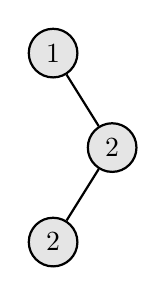
\begin{tikzpicture}
[level distance=12mm, every node/.style={draw, circle,minimum size=6mm, fill=gray!20!},thick]
\node{1}
	child[missing]
	child{node{2} child{node{2}} child[missing]};
\end{tikzpicture}
\end{figure}
\textbf{Output}: 2
\end{flushleft}

\paragraph{Note:} 

\begin{itemize}
\item If a tree has more than one mode, you can return them in any order.
\end{itemize}

\paragraph{Follow up:} 
\begin{itemize}
\item Could you do that without using any extra space? (Assume that the implicit stack space incurred due to recursion does not count).
\end{itemize}

\subsection{Inorder Traverse}
\begin{itemize}
\item 由于是BST,因此inorder遍历的结果是递增序列
\item 这样问题就转换成在递增序列中寻找连续的相同值的个数。
\end{itemize}

\setcounter{lstlisting}{0}
\begin{lstlisting}[style=customc, caption={Inorder Traverse}]
vector<int> findMode( TreeNode* root )
{
    if( !root )
    {
        return {};
    }

    int count = 0;
    int max_count = 0;

    //since at first, count is 1
    //so set last to root-val is safe
    int last = root->val;

    vector<int> ans;

    inorder( root, last, count, max_count, ans );

    return ans;
}

//inorder traverse
void inorder( TreeNode* node, int& last, int& count, int& max_count, vector<int>& modes )
{
    if( !node )
    {
        return;
    }

    inorder( node->left, last, count, max_count, modes );

    if( node->val != last )
    {
        last = node->val;
        count = 1;
    }
    else
    {
        ++count;
    }

    if( count > max_count )
    {
        //new maximum count
        max_count = count;
        //remove all elements in modes
        modes.clear();
        modes.push_back( node->val );
    }
    else if( count == max_count )
    {
        //new element that has maximum count
        modes.push_back( node->val );
    }

    inorder( node->right, last, count, max_count, modes );
}
\end{lstlisting}
%\section{502 --- IPO}
Suppose LeetCode will start its IPO soon. In order to sell a good price of its shares to Venture Capital, LeetCode would like to work on some projects to increase its capital before the IPO. Since it has limited resources, it can only finish at most $k$ distinct projects before the IPO. Help LeetCode design the best way to maximize its total capital after finishing at most k distinct projects.

You are given several projects. For each project $i$, it has a pure profit $P_i$ and a minimum capital of $C_i$ is needed to start the corresponding project. Initially, you have $W$ capital. When you finish a project, you will obtain its pure profit and the profit will be added to your total capital.

To sum up, pick a list of at most $k$ distinct projects from given projects to maximize your final capital, and output your final maximized capital.

\paragraph{Example 1:}

\begin{flushleft}
\textbf{Input}: $k=2$, $W=0$, $P=[1,2,3]$, $C=[0,1,1]$.

\textbf{Output}: 4

\textbf{Explanation}: 

Since your initial capital is 0, you can only start the project indexed 0.

After finishing it you will obtain profit 1 and your capital becomes 1.

With capital 1, you can either start the project indexed 1 or the project indexed 2.

Since you can choose at most 2 projects, you need to finish the project indexed 2 to get the maximum capital.

Therefore, output the final maximized capital, which is $0 + 1 + 3 = 4$.
\end{flushleft}

\paragraph{Note:}

\begin{itemize}
\item You may assume all numbers in the input are non-negative integers.
\item The length of Profits array and Capital array will not exceed 50,000.
\item The answer is guaranteed to fit in a 32-bit signed integer.
\end{itemize}

\subsection{Greedy By Two Priority Queues}
\begin{itemize}
\item We need two priority queues. one is maximum queue $Q_1$ and another minimum queue $Q_2$.
\item Iterate over the profits and capitals, put (captial, profit) pair into the maximum queue $Q_1$. Then the smallest capital project is at the top of $Q_1$
\item Run a loop for $k$ times. At each loop, pop out all pairs with capital $c$ less than or equal to current $W$ and push (profit, capital) pair into $Q_2$.
\item Add the profit to $W$ from top of $Q_2$ which is the maximum profit we can get so far.
\end{itemize}

\setcounter{lstlisting}{0}
\begin{lstlisting}[style=customc, caption={Greedy By Two Prority Queue}]
int findMaximizedCapital( int k, int W, vector<int>& Profits, vector<int>& Capital )
{
    //minimum queue: the largest value is at the top
    priority_queue<pair<int, int>> pq_pros;
    //maximum queue: the smallest value is at the top
    priority_queue<pair<int, int>, vector<pair<int, int>>, greater<pair<int, int>>> pq_caps;

    //put (capital, proift) into maximum priority queue
    //the top of the queue is the minimum capital
    for( size_t i = 0; i < Profits.size(); ++i )
    {
        pq_caps.emplace( Capital[i], Profits[i] );
    }

    for( int i = 0; i < k; ++i )
    {
        //try to remove all projects that
        //has capital requirements less than or
        //equal to W
        while( !pq_caps.empty() )
        {
            if( pq_caps.top().first > W )
            {
                break;
            }

            auto t = pq_caps.top();

            pq_caps.pop();

            //add (profit, capital) into
            //profit queue which has
            //the maximum profit at the top
            pq_pros.emplace( t.second, t.first );
        }

        if( pq_pros.empty() )
        {
            break;
        }

        auto t = pq_pros.top();
        pq_pros.pop();

        //add current maximum profit we get
        //to total captial W
        W += t.first;
    }

    return W;
}
\end{lstlisting}

\subsection{Modified Greedy Without Priority Queue}
\begin{itemize}
\item 上述算法的复杂度为$O(nk\log k)$,而$\log k$来自于prority queue的push和pop操作。
\item 而其实可以通过mark的方法来确定某个project不能够被再次使用,复杂度降为constant。
\item 实际测试时,最后一个test case发生LTE,因此需要先判断是否所有的projects都能够使用。如果所有的projects都可以用,那么直接统计$k$ largest profits即可。
\end{itemize}

\begin{lstlisting}[style=customc, caption={Greedy By Marking}]
int findMaximizedCapital( int k, int W, vector<int>& Profits, vector<int>& Capital )
{

    //first we check if all projects
    //can be used
    //Otherwise, we cannot pass
    //the last testcase
    bool b_all = true;

    for( int cap : Capital )
    {
        if( cap > W )
        {
            b_all = false;
            break;
        }
    }

    if( b_all )
    {
        //if all projects can be used
        //just get k most largest profits
        //projects
        priority_queue<int, vector<int>, greater<int>> pq;

        for( int pro : Profits )
        {
            pq.emplace( pro );

            if( pq.size() > k )
            {
                pq.pop();
            }
        }

        while( !pq.empty() )
        {
            W += pq.top();
            pq.pop();
        }

        return W;
    }

    int L = static_cast<int>( Profits.size() );

    int end = ( min )( k, L );

    for( int i = 0; i < end; ++i )
    {
        int max_profit = 0;
        int sel = -1;

        for( int p = 0; p < L; ++p )
        {
            if( Capital[p] < 0 )
            {
                //project p has been used
                continue;
            }

            if( Capital[p] <= W )
            {
                if( max_profit < Profits[p] )
                {
                    max_profit = Profits[p];
                    sel = p;
                }
            }
        }

        if( sel < 0 )
        {
            break;
        }

        W += max_profit;

        Capital[sel] = -1;
    }

    return W;
}
\end{lstlisting}
%\section{503 --- Next Greater Element II}
Given a circular array $A$ (the next element of the last element is the first element of the array), print the Next Greater Number for every element. The Next Greater Number of a number $x$ is the first greater number to its traversing-order next in the array, which means you could search circularly to find its next greater number. If it doesn't exist, output -1 for this number.

\paragraph{Example 1:}
\begin{flushleft}
\textbf{Input}: $[1,2,1]$

\textbf{Output}: $[2,-1,2]$

\textbf{Explanation}: 

The first 1's next greater number is 2; 

The number 2 can't find next greater number; 

The second 1's next greater number needs to search circularly, which is also 2.
\end{flushleft}

\subsection{Stack}
\begin{itemize}
\item 同Next Greater Element I解法类似,需要一个stack $\Omega$。在stack中保存的是element在数组中的index。
\item 同样先遍历原数组,然后从$\Omega$中弹出所有的小于当前number的element,这些数的next greater element即为当前的number。然后将当前index压入$\Omega$中。
\item 由于array是循环数组,因此还需要再循环一遍,在这次循环中,仍然重复上述过程,但是不再压入新的元素。
\end{itemize}

\setcounter{lstlisting}{0}
\begin{lstlisting}[style=customc, caption={Stack}]
vector<int> nextGreaterElements( vector<int>& nums )
{
    stack<size_t> stk;

    vector<int> ans( nums.size(), -1 );

    for( size_t i = 0; i < nums.size(); ++i )
    {
        //pop all elements in stack
        //that is less than current number
        //these elements' next greater elements
        //is nums[i]
        while( !stk.empty() && ( nums[stk.top()] < nums[i] ) )
        {
            auto t = stk.top();
            ans[t] = nums[i];
            stk.pop();
        }

        //push current index to stack
        stk.push( i );
    }

    //since array is circular
    //we still need to run a loop again to
    //find next greater element in the remaining
    //elements in the stack
    for( size_t i = 0; i < nums.size(); ++i )
    {
        while( !stk.empty() && ( nums[stk.top()] < nums[i] ) )
        {
            auto t = stk.top();
            ans[t] = nums[i];
            stk.pop();
        }

        if( stk.empty() )
        {
            break;
        }
    }

    return ans;
}
\end{lstlisting}
%\section{504 --- Base 7}
Given an integer $n$, return its base 7 string representation.

\paragraph{Example 1:}

\begin{flushleft}
\textbf{Input}: 100

\textbf{Output}: 202

\end{flushleft}

\paragraph{Example 2:}

\begin{flushleft}
\textbf{Input}: $-7$

\textbf{Output}: $-10$
\end{flushleft}

\paragraph{Note:} 

\begin{itemize}
\item The input will be in range of $[-10^{7}, 10^{7}]$.
\end{itemize}

\subsection{Iterative}
每次除以7,余数放入结果字符串,从得到的商继续。

\setcounter{lstlisting}{0}
\begin{lstlisting}[style=customc, caption={Iterative}]
string convertToBase7( int num )
{
    if( num == 0 )
    {
        return "0";
    }

    string ans;

    int n = num;
    int sign = 1;

    if( num < 0 )
    {
        n *= -1;
        sign = -1;
    }

    while( n )
    {
        int q = n / 7;
        int r = n - q * 7;

        ans.push_back( r + '0' );
        n = q;
    }

    if( sign < 0 )
    {
        ans.push_back( '-' );
    }

    //since we add low positions first
    //reverse whole result
    reverse( begin( ans ), end( ans ) );

    return ans;
}
\end{lstlisting}



\subsection{Recursive}
\begin{itemize}
\item $n$可以分为除以7的商和对7的余数两个部分。
\item 分别对这两个部分递归调用函数。
\end{itemize}

\begin{lstlisting}[style=customc, caption={Recursion}]
string convertToBase7( int num )
{
    if( num < 0 )
    {
        return "-" + convertToBase7( -num );
    }

    if( num < 7 )
    {
        //value less than 7 is itself
        return to_string( num );
    }

    return convertToBase7( num / 7 ) + convertToBase7( num % 7 );
}
\end{lstlisting}
%\section{505 --- The Maze II}
There is a ball in a maze with empty spaces and walls. The ball can go through empty spaces by rolling up, down, left or right, but it won't stop rolling until hitting a wall. When the ball stops, it could choose the next direction.

Given the ball's start position $S$, the destination $D$ and the maze $G$, find the shortest distance for the ball to stop at the destination. The distance is defined by the number of empty spaces traveled by the ball from the start position (excluded) to the destination (included). If the ball cannot stop at the destination, return $-1$.

The maze is represented by a binary 2D array. 1 means the wall and 0 means the empty space. You may assume that the borders of the maze are all walls. The start and destination coordinates are represented by row and column indexes.
 

\paragraph{Example 1:}

\begin{flushleft}
\textbf{Input}: 

a maze represented by a 2D array

\begin{table}[H]
\begin{tabular}{ccccc}
0 & 0 & 1 & 0 & 0 \\
0 & 0 & 0 & 0 & 0 \\
0 & 0 & 0 & 1 & 0 \\
1 & 1 & 0 & 1 & 1 \\
0 & 0 & 0 & 0 & 0
\end{tabular}
\end{table}

Sart coordinate: $S = (0, 4)$

Destination coordinate: $D = (4, 4)$

\textbf{Output}: 12

\textbf{Explanation}: 

One shortest way is : left $\longrightarrow$ down $\longrightarrow$ left $\longrightarrow$ down $\longrightarrow$ right $\longrightarrow$ down $\longrightarrow$ right. 

The total distance is $1 + 1 + 3 + 1 + 2 + 2 + 2 = 12$.

\begin{figure}[H]
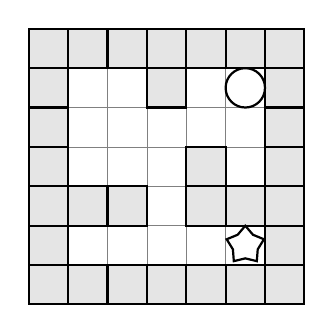
\begin{tikzpicture}
[ thick]
\draw[step=5mm, help lines] (0,0) grid (3.5,3.5);
\foreach \x in {0, 0.5, ..., 3}
{
\draw[fill=gray!20!] (\x,0) rectangle ++(0.5,0.5);
}
\foreach \x in {0.5, 1, ..., 3}
{
\draw[fill=gray!20!] (0, \x) rectangle ++(0.5,0.5);
}

\foreach \x in {0.5, 1,..., 3}
{
\draw[fill=gray!20!] (\x,3) rectangle ++(0.5,0.5);
}

\foreach \x in {0.5, 1,..., 2.5}
{
\draw[fill=gray!20!] (3,\x) rectangle ++(0.5,0.5);
}

\draw[fill=gray!20!] (1.5, 2.5) rectangle ++(0.5,0.5);
\draw[fill=gray!20!] (0.5, 1) rectangle ++(0.5,0.5);
\draw[fill=gray!20!] (1, 1) rectangle ++(0.5,0.5);
\draw[fill=gray!20!] (2, 1) rectangle ++(0.5,0.5);
\draw[fill=gray!20!] (2.5, 1) rectangle ++(0.5,0.5);
\draw[fill=gray!20!] (2, 1.5) rectangle ++(0.5,0.5);
\node[star, minimum size=0.2cm, draw] at (2.75, 0.75) {};
\draw (2.75, 2.75) circle (0.25cm);
\end{tikzpicture}
\end{figure}
\end{flushleft}

\paragraph{Example 2:}

\begin{flushleft}
\textbf{Input}: a maze represented by a 2D array

\begin{table}[H]
\begin{tabular}{ccccc}
0 & 0 & 1 & 0 & 0 \\
0 & 0 & 0 & 0 & 0 \\
0 & 0 & 0 & 1 & 0 \\
1 & 1 & 0 & 1 & 1 \\
0 & 0 & 0 & 0 & 0
\end{tabular}
\end{table}

Start coordinate: $S = (0, 4)$

Destination coordinate: $D = (3, 2)$

\textbf{Output}: $-1$

\textbf{Explanation}: 

There is no way for the ball to stop at the destination.


\begin{figure}[H]
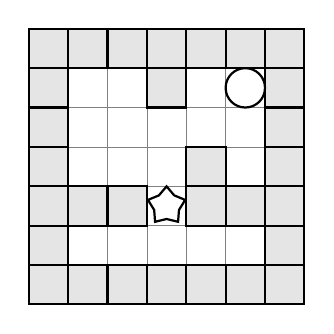
\begin{tikzpicture}
[ thick]
\draw[step=5mm, help lines] (0,0) grid (3.5,3.5);
\foreach \x in {0, 0.5, ..., 3}
{
\draw[fill=gray!20!] (\x,0) rectangle ++(0.5,0.5);
}
\foreach \x in {0.5, 1, ..., 3}
{
\draw[fill=gray!20!] (0, \x) rectangle ++(0.5,0.5);
}

\foreach \x in {0.5, 1,..., 3}
{
\draw[fill=gray!20!] (\x,3) rectangle ++(0.5,0.5);
}

\foreach \x in {0.5, 1,..., 2.5}
{
\draw[fill=gray!20!] (3,\x) rectangle ++(0.5,0.5);
}

\draw[fill=gray!20!] (1.5, 2.5) rectangle ++(0.5,0.5);
\draw[fill=gray!20!] (0.5, 1) rectangle ++(0.5,0.5);
\draw[fill=gray!20!] (1, 1) rectangle ++(0.5,0.5);
\draw[fill=gray!20!] (2, 1) rectangle ++(0.5,0.5);
\draw[fill=gray!20!] (2.5, 1) rectangle ++(0.5,0.5);
\draw[fill=gray!20!] (2, 1.5) rectangle ++(0.5,0.5);
\node[star, minimum size=0.2cm, draw] at (1.75, 1.25) {};
\draw (2.75, 2.75) circle (0.25cm);
\end{tikzpicture}
\end{figure}

\end{flushleft}
 

\paragraph{Note:}

\begin{itemize}
\item There is only one ball and one destination in the maze.
\item Both the ball and the destination exist on an empty space, and they will not be at the same position initially.
\item The given maze does not contain border (like the red rectangle in the example pictures), but you could assume the border of the maze are all walls.
\item The maze contains at least 2 empty spaces, and both the width and height of the maze won't exceed 100.
\end{itemize}

\subsection{Depth First Search}
\begin{itemize}
\item 需要maintain一个和maze大小相同的array $D$,用于记录每个位置从开始位置出发的最小距离。
\item 从当前位置出发,一直move下去。直到遇到wall或者越界,然后回到发生越界或者遇到wall的前的最后一个节点,如果这时候这个节点到出发点的距离比在$D$中记录的还要小,则将该节点的距离更新为当前距离,然后继续递归下去。
\end{itemize}

\setcounter{lstlisting}{0}
\begin{lstlisting}[style=customc, caption={DFS}]
int shortestDistance( vector<vector<int>>& maze, vector<int>& start, vector<int>& destination )
{
    //records each node's minimum distance
    //to the start node
    vector<vector<int>> dists( maze.size(), vector<int>( maze[0].size(), INT_MAX ) );
    dists[start[0]][start[1]] = 0;

    dfs( maze, dists, start[0], start[1], destination );

    int x = dists[destination[0]][destination[1]];
    return x == INT_MAX ? -1 : x;
}


void dfs( vector<vector<int>>& G, vector<vector<int>>& dists, int r, int c, vector<int>& dest )
{
    if( ( r == dest[0] ) && ( c == dest[1] ) )
    {
        //we are at the destination
        return;
    }

    int dr[] = {-1, 0, 1, 0};
    int dc[] = {0, -1, 0, 1};

    int m = static_cast<int>( G.size() );
    int n = static_cast<int>( G[0].size() );

    //test each possible direction
    for( int i = 0; i < 4; ++i )
    {
        int nr = r;
        int nc = c;

        int dist = dists[r][c];

        while( ( nr >= 0 ) && ( nr < m ) && ( nc >= 0 ) && ( nc < n ) && ( G[nr][nc] == 0 ) )
        {
            nr += dr[i];
            nc += dc[i];

            ++dist;
        }

        //back off to the
        //last node before
        //over the bounday or hit the wall

        nr -= dr[i];
        nc -= dc[i];

        --dist;

        int x = dists[nr][nc];

        if( dist < x )
        {
            //only do recursive when
            //dist is less than the recorded distance
            //for (nr,nc)
            dists[nr][nc] = dist;
            dfs( G, dists, nr, nc, dest );
        }
    }
}
\end{lstlisting}

\subsection{BFS}
Instead of making use of DFS for exploring the search space, we can make use of BFS as well. In this approach, instead of exploring the search space on a depth basis, we traverse the search space(tree) on a level by level basis i.e. we explore all the new positions that can be reached starting from the current position first, before moving onto the next positions that can be reached from these new positions.

\setcounter{lstlisting}{0}
\begin{lstlisting}[style=customc, caption={BFS}]
int shortestDistance( vector<vector<int>>& maze, vector<int>& start, vector<int>& destination )
{

    //BFS
    using node_t = array<int, 2>;
    queue<node_t> q;

    //the distance array to record minimum distance from
    //start to each position
    vector<vector<int>> dists( maze.size(), vector<int>( maze[0].size(), INT_MAX ) );
    dists[start[0]][start[1]] = 0;

    q.push( node_t{start[0], start[1]} );

    //directions offsets
    array<int, 4> dr( {-1, 0, 1, 0} );
    array<int, 4> dc( {0, -1, 0, 1} );

    int m = static_cast<int>( maze.size() );
    int n = static_cast<int>( maze[0].size() );

    while( !q.empty() )
    {
        auto t = q.front();
        q.pop();

        int r = t[0];
        int c = t[1];


        for( int i = 0; i < 4; ++i )
        {
            int nr = r;
            int nc = c;

            int dist = dists[nr][nc];

            //rolling the ball until
            //hitting the wall or
            //out of boundary
            while( ( nr >= 0 ) && ( nr < m ) && ( nc >= 0 ) && ( nc < n ) && ( maze[nr][nc] == 0 ) )
            {
                nr += dr[i];
                nc += dc[i];
                ++dist;
            }

            //backward to last node before hitting the wall
            //or out of boundary
            nr -= dr[i];
            nc -= dc[i];
            --dist;

            if( dist < dists[nr][nc] )
            {
                //only when we get a less distance
                //from start, then push to the queue
                dists[nr][nc] = dist;
                q.emplace( node_t{nr, nc} );
            }
        } //end for
    }//end while

    int x = dists[destination[0]][destination[1]];
    return x == INT_MAX ? -1 : x;
}
\end{lstlisting}

\subsection{Dijkstra Algorithm}

The given problem is also a shortest distance finding problem with a slightly different set of rules. Thus, we can make use of Dijkstra's Algorithm to determine the minimum number of steps to reach the destination.

The methodology remains the same as the \textbf{DFS} or \textbf{BFS} Approach discussed above, except the order in which the current positions are chosen. We again make use of an array $D$ to keep a track of the minimum number of steps needed to reach every position from the \textit{start} position. At every step, we choose a position which hasn't been marked as \textbf{visited} and which is at the shortest distance from the \textit{start} position to be the current position. We mark this position as visited so that we don't consider this position as the current position again.

To do the above operations efficiently, we can make use of a priority queue, $Q$. This priority queue is a maximum queue: the top element is the node which is unvisited and at the smallest distance from the \textit{start} node. Thus, the node to be chosen as the current node, is always at the top of $Q$.

For every current node, we again try to traverse in all the possible directions. We determine the minimum number of steps(till now) required to reach all the end points possible from the current node. If any such end point can be reached in a less number of steps through the current path than the paths previously considered, we need to update its distance entry in array $D$.

Further, we add an entry corresponding to this node in $Q$, since its distance entry has been updated and we need to consider this node as the competitors for the next current node choice. Thus, the process remains the same as the last approach, except the way in which the pick out the current node (which is the unvisited node at the shortest distance from the \textit{start} node).

\begin{lstlisting}[style=customc, caption={Dijkastra Algorithm}]
int shortestDistance( vector<vector<int>>& maze, vector<int>& start, vector<int>& destination )
{
    auto cmp = []( const array<int, 3>& a1, const array<int, 3>& a2 )
    {
        return a1[2] > a2[2];
    };

    //maximum priority queue for Dijkastra
    priority_queue<array<int, 3>, vector<array<int, 3>>, decltype( cmp )> pq( cmp );

    pq.emplace( array<int, 3> {start[0], start[1], 0} );

    //We still need this 2d array
    //to record each position's minimum distance from start
    vector<vector<int>> dists( maze.size(), vector<int>( maze[0].size(), INT_MAX ) );
    dists[start[0]][start[1]] = 0;

    array<int, 4> dr( {-1, 0, 1, 0} );
    array<int, 4> dc( {0, -1, 0, 1} );

    int m = static_cast<int>( maze.size() );
    int n = static_cast<int>( maze[0].size() );

    while( !pq.empty() )
    {
        auto t = pq.top();
        pq.pop();

        if( dists[t[0]][t[1]] < t[2] )
        {
            //(t[0],t[1]) distance recorded
            //is less than the calculated
            //ignore
            continue;
        }

        int r = t[0];
        int c = t[1];


        for( int i = 0; i < 4; ++i )
        {
            int nr = r;
            int nc = c;
            int dist = dists[r][c];

            while( ( nr >= 0 ) && ( nr < m ) && ( nc >= 0 ) && ( nc < n ) && ( maze[nr][nc] == 0 ) )
            {
                nr += dr[i];
                nc += dc[i];
                ++dist;
            }

            //back to the last node
            //before hitting the wall
            //or out of boundary
            nr -= dr[i];
            nc -= dc[i];
            --dist;

            if( dist < dists[nr][nc] )
            {
                //only push to queue
                //when a less distance is
                //found
                dists[nr][nc] = dist;
                pq.emplace( array<int, 3> {nr, nc, dist} );
            }
        }
    }

    int x = dists[destination[0]][destination[1]];

    return x == INT_MAX ? -1 : x;
}
\end{lstlisting}

\subsection{Overview Of Dijkastra Algorithm}
Dijkstra's Algorithm is a very famous graph algorithm, which is used to find the shortest path from any start node to any destination node in the given weighted graph(the edges of the graph represent the distance between the nodes).

The algorithm consists of the following steps:
\begin{enumerate}
\item Assign a tentative distance value to every node: set it to zero for our start node and to $\infty$ for all other nodes.
\item Set the start node as current node. Mark it as visited.
\item For the current node, consider all of its neighbors and calculate their tentative distances. Compare the newly calculated tentative distance to the current assigned value and assign the smaller one to all the neighbors. For example, if the current node $A$ is marked with a distance of 6, and the edge connecting it with a neighbor $B$ has length 2, then the distance to $B$ (through $A$) will be $6 + 2 = 8$. If $B$ was previously marked with a distance greater than 8 then change it to 8. Otherwise, keep the current value.
\item When we are done considering all of the neighbors of the current node, mark the current node as visited. A visited node will never be checked again.
\item If the destination node has been marked \textbf{visited} or if the \textbf{smallest} tentative distance among all the nodes left is $\infty$ (indicating that the destination can't be reached), then stop. The algorithm has finished.
\item Otherwise, select the \textit{unvisited} node that is marked with the smallest tentative distance, set it as the new \textbf{current} node, and go back to step 3.
\end{enumerate}

The working of this algorithm can be understood by taking two simple examples. Consider the first set of nodes as shown below.

\begin{figure}[H]
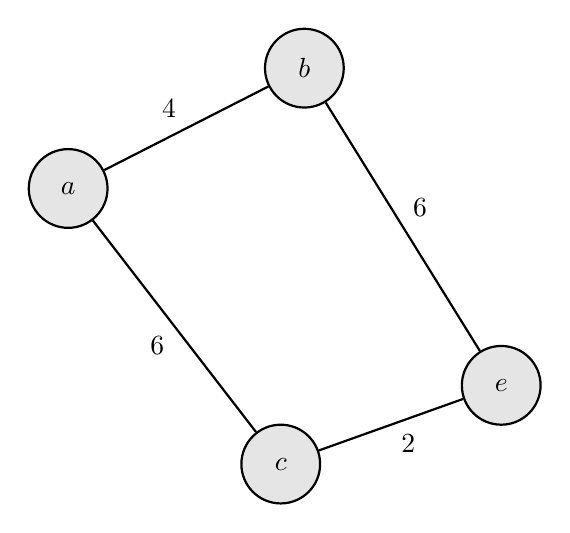
\begin{tikzpicture}
[my/.style={draw, circle,
 minimum size=1cm, fill=gray!20!},
 thick
]

\node[my](a) at(0,0) {$a$};
\node[my](b) [above=0.5cm of a, xshift=3cm] {$b$};
\node[my](c) [below=3cm of b, xshift=2.5cm] {$e$};
\node[my](d) [below=4cm of b, xshift=-0.3cm] {$c$};
\draw (a) -- (b) node[pos=0.5, auto] {4};
\draw (b) -- (c) node[pos=0.5, auto] {6};
\draw (c) -- (d) node[pos=0.5, auto] {2};
\draw (d) -- (a) node[pos=0.5, auto] {6};
\end{tikzpicture}
\end{figure}

Suppose that the node $b$ is at a shorter distance from the start node $a$ as compared to $c$, but the distance from $a$ to the destination node, $e$, is shorter through the node $c$ itself. In this case, we need to check if the \textbf{Dijkstra}'s algorithm works correctly, since the node $b$ is considered first while selecting the nodes being at a shorter distance from $a$. Let's look into this.

\begin{enumerate}
\item Firstly, we choose $a$ as the start node, mark it as \textit{visited} and update the distance values of $b$ and $c$, say $D_b$ and $D_c$.
\item Since $D_b < D_c$, $b$ is chosen as the next node for calculating the distances. We mark $b$ as \textit{visited}. Now, we update the distance value of $e$, $D_e$, as $D_b+W(b,e)$ where $W(b,e)$ is the weight from $b$ to $e$.
\item Now, $c$ is obviously the next node to be chosen because $D_c < D_b + W(b,e)$. From $c$, we determine the distance to node $e$. Since $D_c+ W(c, e) < D_e$, we update $D_e$ as this shorter value.
\item We choose $e$ as the current node. No other distances need to be updated. Thus, we mark $e$ as visited. $D_e$  now gives the required shortest distance.
\end{enumerate}

The above example proves that even if a locally closer node is chosen as the current node first, the ultimate shortest distance to any node is calculated correctly.

Let's take another example to demonstrate that the visited node needs not be chosen again as the current node.

\begin{figure}[H]
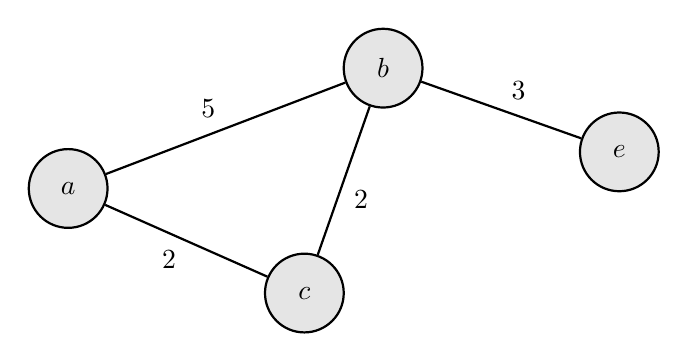
\begin{tikzpicture}
[my/.style={draw, circle,
 minimum size=1cm, fill=gray!20!},
 thick
]

\node[my](a) at(0,0) {$a$};
\node[my](b) [above=0.5cm of a, xshift=4cm] {$b$};
\node[my](c) [below=0.3cm of a, xshift=3cm] {$c$};
\node[my](d) [below=1pt of b, xshift=3cm] {$e$};
\draw (a) -- (b) node[pos=0.5, auto] {5};
\draw (b) -- (c) node[pos=0.5, auto] {2};
\draw (c) -- (a) node[pos=0.5, auto] {2};
\draw (b) -- (d) node[pos=0.5, auto] {3};
\end{tikzpicture}
\end{figure}


Suppose $a$ is the start node and $e$ is the destination node. Now, suppose we visit $b$ first and mark it as visited, but later on we find that another path exists through $c$ to $b$, which makes the distance value of $b$, $D_b$, shorter than the previous value. But, because of this, we need to consider $b$ as the current node again, since it would affect the value of $D_e$. But, if we observe closely, such a situation would never occur, because $W(a,c) + W(c,b) < W(a,b)$ and $W(a,c) < W(a,b)$ in the first place. Thus, $b$ would never be marked \textbf{visited} before $c$, which contradicts the first assumption. This proves that the \textit{visited} node needs not be chosen as the current node again.


%\section{506 --- Relative Ranks}
Given scores of $N$ athletes, find their relative ranks and the people with the top three highest scores, who will be awarded medals: \textbf{Gold Medal}, \textbf{Silver Medal} and \textbf{Bronze Medal}.

\paragraph{Example 1:}

\begin{flushleft}
\textbf{Input}: $[5, 4, 3, 2, 1]$

\textbf{Output}: [Gold Medal, Silver Medal, Bronze Medal, 4, 5]

\textbf{Explanation}: 

The first three athletes got the top three highest scores, so they got Gold Medal, Silver Medal and Bronze Medal. 

For the left two athletes, you just need to output their relative ranks according to their scores.
\end{flushleft}

\paragraph{Note:}
\begin{itemize}
\item $N$ is a positive integer and won't exceed 10,000.
\item All the scores of athletes are guaranteed to be unique.
\end{itemize}

\subsection{Priority Queue}
其实就是找到排序后原来的元素在排序后的位置。可以用priority queue作为数据结构。

\setcounter{lstlisting}{0}
\begin{lstlisting}[style=customc, caption={Priority Queue}]
vector<string> findRelativeRanks( vector<int>& nums )
{
    priority_queue<pair<int, size_t>> pq;

    for( size_t i = 0; i < nums.size(); ++i )
    {
        pq.emplace( nums[i], i );
    }

    vector<string> ans( nums.size() );

    if( !pq.empty() )
    {
        auto t = pq.top();
        ans[t.second] = "Gold Medal";
        pq.pop();
    }

    if( !pq.empty() )
    {
        auto t = pq.top();
        ans[t.second] = "Silver Medal";
        pq.pop();
    }

    if( !pq.empty() )
    {
        auto t = pq.top();
        ans[t.second] = "Bronze Medal";
        pq.pop();
    }

    int next = 4;

    while( !pq.empty() )
    {
        auto t = pq.top();
        pq.pop();
        ans[t.second] = to_string( next );
        ++next;
    }

    return ans;
}
\end{lstlisting}
%\section{507 --- Perfect Number}
We define the Perfect Number is a positive integer that is equal to the sum of all its positive divisors except itself.

Now, given an integer $n$, write a function that returns true when it is a perfect number and false when it is not.

\paragraph{Example:}

\begin{flushleft}
\textbf{Input}: 28

\textbf{Output}: \texttt{true}

\textbf{Explanation}: $28 = 1 + 2 + 4 + 7 + 14$
\end{flushleft}

\paragraph{Note:} 
\begin{itemize}
\item The input number n will not exceed 100,000,000. $(10^8)$
\end{itemize}

\subsection{Optimal Solution}
\begin{itemize}
\item Suppose the given number $n$ has $m$ distinct factors, $f_1, f_2, \ldots, f_m$. 
\item Since the number $n$ divisible by $f_i$, it is also divisible by $f_j=n/f_i$.
\item Also, the largest number in such a pair can only be up to $\sqrt{n}$ ( because $\sqrt{n} \times \sqrt{n}=n$ ). Thus, we can get a significant reduction in the run-time by iterating only up to $\sqrt{n}$ and get such $f_i$ and $f_j$ in a single pass directly.
\item \textbf{Note}: If $\sqrt{n}$ is also a factor, we have to consider the factor only once. 
\item \textbf{Note}: While considering 1 as such a factor, $n$ will also be considered as the other factor. Thus, we need to subtract $n$ from the sum.
\end{itemize}

\setcounter{lstlisting}{0}
\begin{lstlisting}[style=customc, caption={Optimal Approach}]
bool checkPerfectNumber( int num )
{
    if( num <= 0 )
    {
        return false;
    }

    int sum = 0;

    //only up to sqrt(num)
    for( int i = 1; i * i <= num; ++i )
    {
        int q = num / i; //factor pair(i, q)
        int r = num - q * i;

        if( r == 0 )
        {
            if( q != i )
            {
                sum += q;
                sum += i;
            }
        }
    }

    //for factor 1, the factor pair is (1, num)
    //so need to subtract num from sum
    return sum - num == num;
}
\end{lstlisting}
%\section{508 --- Most Frequent Subtree Sum}
Given the root of a tree, you are asked to find the most frequent subtree sum. The subtree sum of a node is defined as the sum of all the node values formed by the subtree rooted at that node (including the node itself). So what is the most frequent subtree sum value? If there is a tie, return all the values with the highest frequency in any order.

\paragraph{Examples 1}
\begin{flushleft}
\textbf{Input}:
\begin{figure}[H]
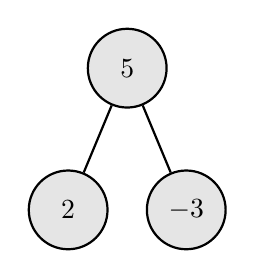
\begin{tikzpicture}
[every node/.style={draw, circle,
 minimum size=10mm, fill=gray!20!},
  level distance=18mm, 
 thick
]
\node{5}
	child{node{2}}
	child{node{$-3$}};
\end{tikzpicture}
\end{figure}
\textbf{Output}: $[2, -3, 4]$

\textbf{Explanation}:

Since all the values happen only once, return all of them in any order.
\end{flushleft}

\paragraph{Examples 2}
\begin{flushleft}
\textbf{Input}:
\begin{figure}[H]
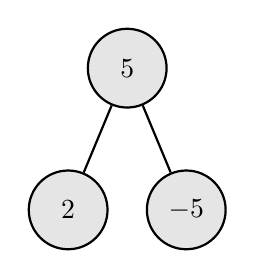
\begin{tikzpicture}
[every node/.style={draw, circle,minimum size=10mm, fill=gray!20!},level distance=18mm, thick
]
\node{5}
	child{node{2}}
	child{node{$-5$}};
\end{tikzpicture}
\end{figure}

\textbf{Output}: $[2]$

\textbf{Explanation}:

Since 2 happens twice, however $-5$ only occur once.
\end{flushleft}

\paragraph{Note:} 

\begin{itemize}
\item You may assume the sum of values in any subtree is in the range of 32-bit signed integer.
\end{itemize}

\subsection{Recursive}
\begin{itemize}
\item 对于每一个node,其total sum可分解为左右子树的sum加上其自身的value。
\item Maintain a hash map which maps the sum and the counts。
\item Maintain a variable, $x$, to track the maximum count of sums.
\end{itemize}

\setcounter{lstlisting}{0}
\begin{lstlisting}[style=customc, caption={Recursion}]
vector<int> findFrequentTreeSum( TreeNode* root )
{

    vector<int> ans;
    unordered_map<int, int> m;
    int max_count = 0;

    dfs( root, max_count, ans, m );

    return ans;
}
//recursion helper function
int dfs( TreeNode* node, int& max_count, vector<int>& ans, unordered_map<int, int>& m )
{
    if( !node )
    {
        return 0;
    }

    int sum = node->val;
    int left_sum = 0;


    //get left substree sum
    if( node->left )
    {
        left_sum = dfs( node->left, max_count, ans, m );
    }

    int right_sum = 0;

    //get right substree sum
    if( node->right )
    {
        right_sum = dfs( node->right, max_count, ans, m );
    }

    sum += left_sum;
    sum += right_sum;

    //track the maximum count of sums
    //and put (sum, count) into hash map
    int count = 1;
    auto it = m.find( sum );

    if( it != m.end() )
    {
        ++it->second;
        count = it->second;
    }
    else
    {
        m.emplace( sum, 1 );
    }

    if( count > max_count )
    {
        max_count = count;
        ans.clear();
        ans.push_back( sum );
    }
    else if( count == max_count )
    {
        ans.push_back( sum );
    }

    return sum;
}
\end{lstlisting}

%\section{509 --- Fibonacci Number}
The Fibonacci numbers, commonly denoted $F(n)$ form a sequence, called the Fibonacci sequence, such that each number is the sum of the two preceding ones, starting from 0 and 1. That is,
\begin{align*}
F(0) &= 0 \\
F(1) &= 1 \\
F(N) &= F(N - 1) + F(N - 2) \quad N > 1.
\end{align*}

Given $N$, calculate $F(N)$.

\paragraph{Note:}

\begin{itemize}
\item $0 \leq N \leq 30$.
\end{itemize}

\subsection{Dynamic Programming}
\begin{itemize}
\item classical dynamic programming problem.
\item Since $F(N)$ depends only on $F(N-1)$ and $F(N-2)$, we can use two variables $x$ and $y$ to replace.
\end{itemize}

\setcounter{lstlisting}{0}
\begin{lstlisting}[style=customc, caption={Dynamic Programming}]
int fib( int N )
{
    if( N <= 1 )
    {
        return N;
    }

    int x = 0;
    int y = 1;

    for( int i = 2; i <= N; ++i )
    {
        int z = x + y;
        //update F[N-2]
        x = y;
        //update F[N-1]
        y = z;
    }

    return y;
}
\end{lstlisting}
\section{510 --- Inorder Successor in BST II}
Given a binary search tree and a node in it, find the in-order successor of that node in the BST.

The successor of a node $p$ is the node with the smallest key greater than the value of $p$.

You will have direct access to the node but not to the root of the tree. Each node will have a reference to its parent node.
 

\paragraph{Example 1:}

\begin{flushleft}

\textbf{Input}:

\begin{figure}[H]
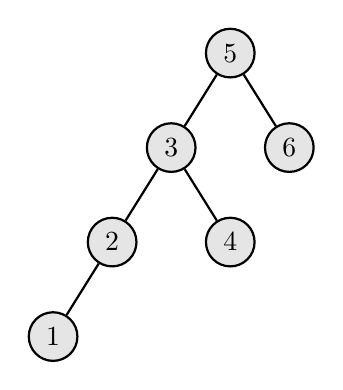
\begin{tikzpicture}
[every node/.style={draw, circle,minimum size=6mm, fill=gray!20!},
  level distance=12mm,  thick]
\node{5}
  child{node{3} child{node{2} child{node{1}} child[missing]} child{node{4}}}
  child{node{6}};
\end{tikzpicture}
\end{figure}
 
$ p = 1 $

\textbf{Output}: 2

\textbf{Explanation}: 

1's in-order successor node is 2. Note that both $p$ and the return value is of Node type.
\end{flushleft}

\paragraph{Example 2:}

\begin{flushleft}
\textbf{Input}: 
\begin{figure}[H]
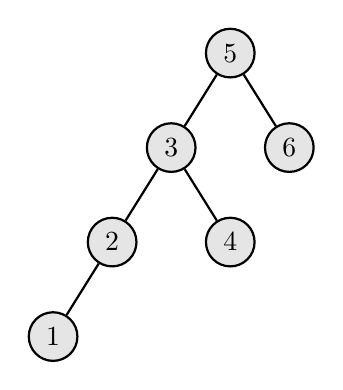
\begin{tikzpicture}
[every node/.style={draw, circle,minimum size=6mm, fill=gray!20!},
  level distance=12mm,  thick]
\node{5}
  child{node{3} child{node{2} child{node{1}} child[missing]} child{node{4}}}
  child{node{6}};
\end{tikzpicture}
\end{figure}
$ p = 6 $

\textbf{Output}: $\emptyset$

\textbf{Explanation}: 

There is no in-order successor of the current node, so the answer is $\emptyset$.
\end{flushleft}

\paragraph{Example 3:}

\begin{flushleft}

\textbf{Input}:
\begin{figure}[H]
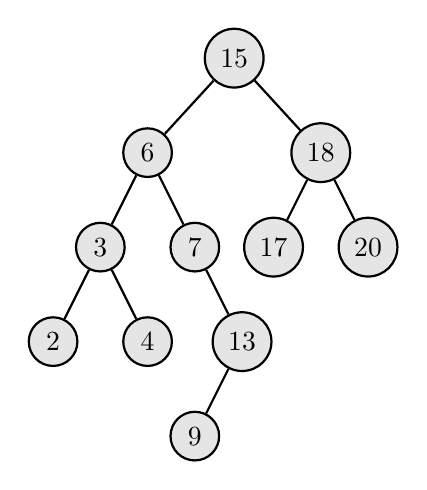
\begin{tikzpicture}
[every node/.style={draw, circle,minimum size=6mm, fill=gray!20!},
  level distance=12mm,  thick, level 1/.style={sibling distance=22mm}, level 2/.style={sibling distance=12mm}]
\node{15}
  child{node{6} child{node{3} child{node{2}} child{node{4}}} child{node{7} child[missing] child{node{13} child{node{9}} child[missing]}}}
  child{node{18} child{node{17}} child{node{20}}};
\end{tikzpicture}
\end{figure}
 
$ p = 15 $


\textbf{Output}: 17

\end{flushleft}

\paragraph{Example 4:}

\begin{flushleft}

\textbf{Input}: 
\begin{figure}[H]
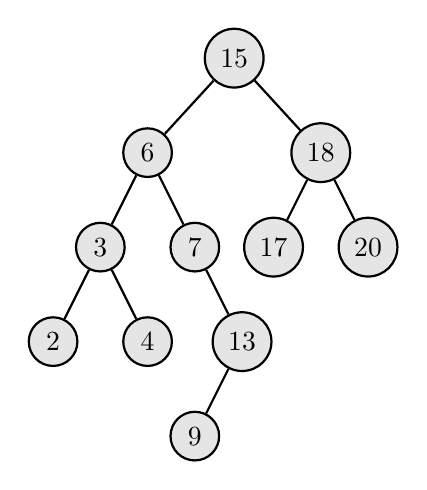
\begin{tikzpicture}
[every node/.style={draw, circle,minimum size=6mm, fill=gray!20!},
  level distance=12mm,  thick, level 1/.style={sibling distance=22mm}, level 2/.style={sibling distance=12mm}]
\node{15}
  child{node{6} child{node{3} child{node{2}} child{node{4}}} child{node{7} child[missing] child{node{13} child{node{9}} child[missing]}}}
  child{node{18} child{node{17}} child{node{20}}};
\end{tikzpicture}
\end{figure}

$ p = 13 $

\textbf{Output}: 15
\end{flushleft}
 

\paragraph{Note:}

\begin{itemize}
\item If the given node has no in-order successor in the tree, return $\emptyset$.
\item It's guaranteed that the values of the tree are unique.
\item Remember that we are using the \textbf{Node} type instead of \textbf{TreeNode} type so their string representation are different.
\end{itemize} 

\paragraph{Follow up:}

\begin{itemize}
\item Could you solve it without looking up any of the node's values?
\end{itemize}

\subsection{Iteration}
在BST中,一个node在inorder traverse的successor node取决于该node是否有right child

\begin{itemize}
\item Has a \textbf{right} child: the successor node is somewhere lower in the tree. To find the successor, go to the right once and then go left always.

For example: The following binary tree's inorder traverse sequence is 1, 2, 7, 11, 12, 13, 25, 33, 34, 36, 40. The node 33' successor is 34.
\begin{figure}[H]
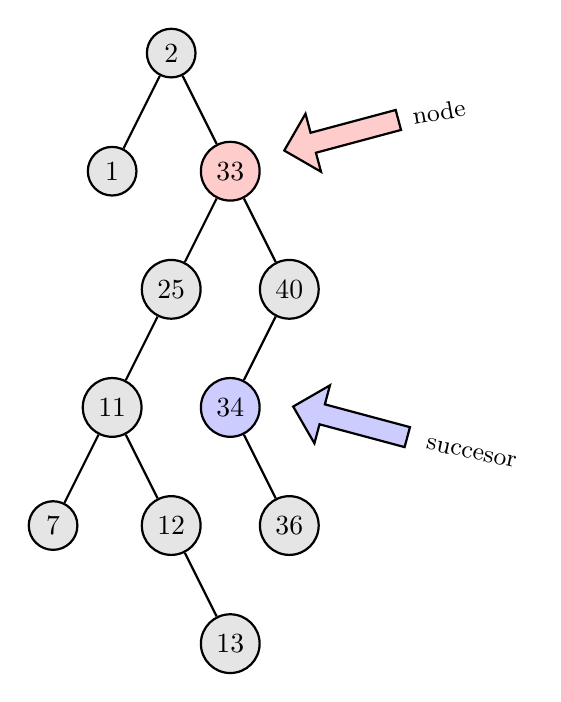
\begin{tikzpicture}
[every node/.style={draw, circle,minimum size=6mm, fill=gray!20!},node distance=8mm, thick]
\node{2}
child{node{1}}
child{node[fill=red!20!](a){33} 
		child{node{25} child{node{11} child{node{7}} child{node{12} child[missing] child{node{13}}} } child[missing]} 
		child{node{40} child{node(b)[fill=blue!20!]{34} child[missing] child{node{36}}} child[missing]}
	};
\node[single arrow, rotate=195, minimum height=1.5cm, fill=red!20!](r1) at ($(a.north east) + (1.2,0.2)$) {};
\node[draw=none,fill=none, rotate=10] at ($(r1.west) + (0.5,0.1)$) {\small node};
\node[single arrow, rotate=165, minimum height=1.5cm, fill=blue!20!](r2) at($(b.east) + (1.2,-0.2)$) {};
\node[draw=none,fill=none, rotate=-12] at ($(r2.west) + (0.8,-0.2)$) {\small succesor};
\end{tikzpicture}
\caption{Successor of the node with a right child: one step right and then left till you can.}
\end{figure}
\item No right child: the successor is somewhere upper in the tree. To find the successor, go up till the node that is left child of its parent. The answer is the parent. Beware that there could be no successor in such a situation.

\begin{figure}[H]
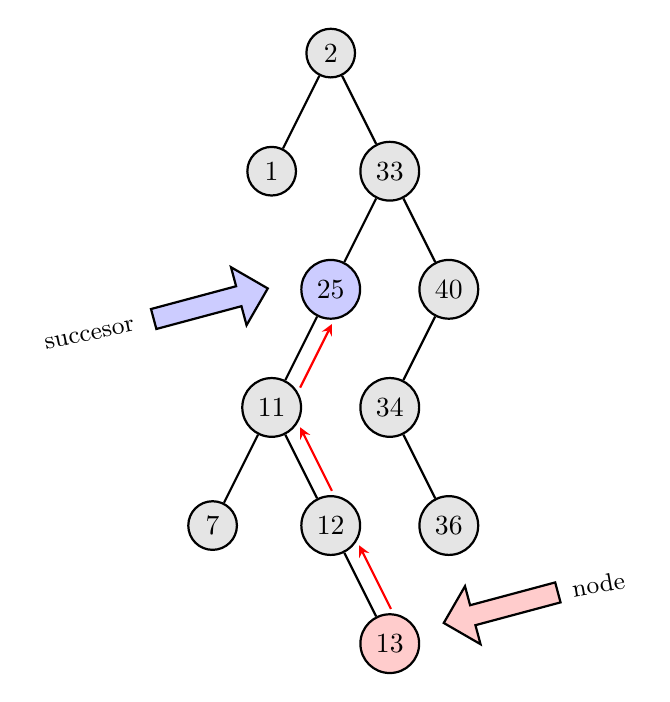
\begin{tikzpicture}
[every node/.style={draw, circle,minimum size=6mm, fill=gray!20!},node distance=8mm, thick]
\node{2}
child{node{1}}
child{node{33} 
		child{node(b)[fill=blue!20!]{25} child{node(p2){11} child{node{7}} child{node(p1){12} child[missing] child{node[fill=red!20!](a){13}}} } child[missing]} 
		child{node{40} child{node{34} child[missing] child{node{36}}} child[missing]}
	};
\node[single arrow, rotate=195, minimum height=1.5cm, fill=red!20!](r1) at ($(a.north east) + (1.2,0.2)$) {};
\node[draw=none,fill=none, rotate=10] at ($(r1.west) + (0.5,0.1)$) {\small node};
\node[single arrow, rotate=15, minimum height=1.5cm, fill=blue!20!](r2) at($(b.west) + (-1.2,-0.2)$) {};
\node[draw=none,fill=none, rotate=12] at ($(r2.west) + (-0.8,-0.2)$) {\small succesor};
\path (a)--(p1)coordinate[at start](h1)coordinate[at end](h2);
\draw[red, >=stealth, ->] ($(h1)!-6pt!90:(h2)$)--($(h2)!-6pt!-90:(h1)$);
\path (p1)--(p2)coordinate[at start](h3)coordinate[at end](h4);
\draw[red, >=stealth, ->] ($(h3)!-6pt!90:(h4)$)--($(h4)!-6pt!-90:(h3)$);
\path (p2)--(b)coordinate[at start](h5)coordinate[at end](h6);
\draw[red, >=stealth, ->] ($(h5)!-6pt!90:(h6)$)--($(h6)!-6pt!-90:(h5)$);
\end{tikzpicture}
\caption{Successor of the node without right child: Go up till the node that is the \textbf{left} child of its parent, then return the parent}
\end{figure}

The following case is an example of null successor.
\begin{figure}[H]
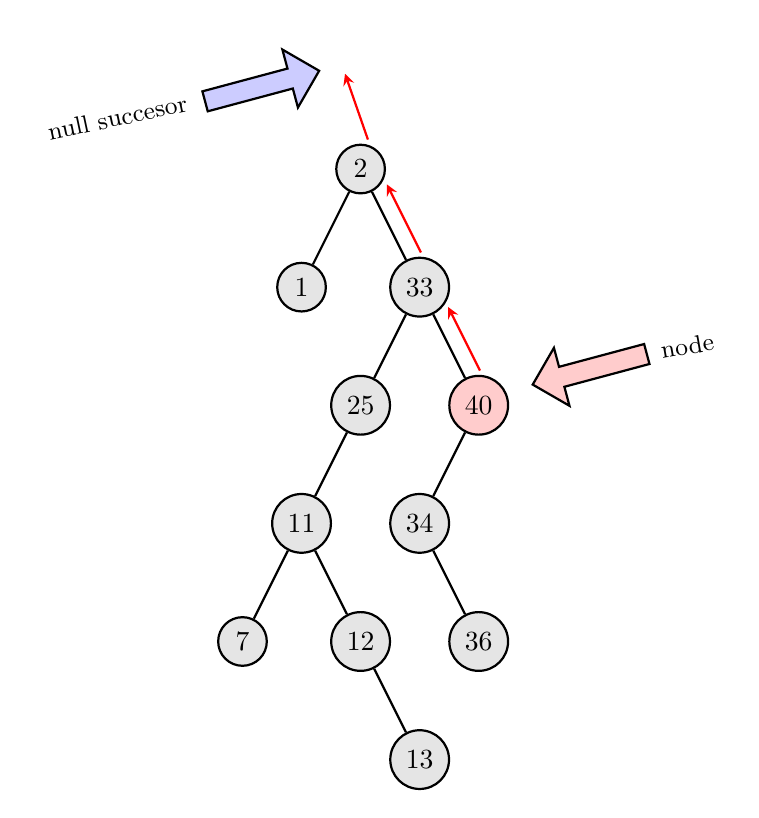
\begin{tikzpicture}
[every node/.style={draw, circle,minimum size=6mm, fill=gray!20!},node distance=8mm, thick]
\node(p2){2}
child{node{1}}
child{node(p1){33} 
		child{node{25} child{node{11} child{node{7}} child{node{12} child[missing] child{node{13}}} } child[missing]} 
		child{node[fill=red!20!](a){40} child{node{34} child[missing] child{node{36}}} child[missing]}
	};
\node[single arrow, rotate=195, minimum height=1.5cm, fill=red!20!](r1) at ($(a.north east) + (1.2,0.2)$) {};
\node[draw=none,fill=none, rotate=10] at ($(r1.west) + (0.5,0.1)$) {\small node};
\path (a)--(p1)coordinate[at start](h1)coordinate[at end](h2);
\draw[red, >=stealth, ->] ($(h1)!-6pt!90:(h2)$)--($(h2)!-6pt!-90:(h1)$);
\path (p1)--(p2)coordinate[at start](h3)coordinate[at end](h4);
\draw[red, >=stealth, ->] ($(h3)!-6pt!90:(h4)$)--($(h4)!-6pt!-90:(h3)$);
\node[draw=none, fill=none](t) [above = 8mm of p2, xshift=-5mm] {};
\path (p2)--(t)coordinate[at start](h5)coordinate[at end](h6);
\draw[red, >=stealth, ->] ($(h5)!-6pt!90:(h6)$)--($(h6)!-6pt!-90:(h5)$);
\node[single arrow, rotate=15, minimum height=1.5cm, fill=blue!20!](r2) at($(t.west) + (-0.5,-0.4)$) {};
\node[draw=none,fill=none, rotate=12] at ($(r2.west) + (-1.1,-0.2)$) {\small null succesor};
\end{tikzpicture}
\caption{Successor of the node without right child: Go up till the node that is the \textbf{left} child of its parent, then return the parent}
\end{figure}

\end{itemize}


\setcounter{lstlisting}{0}
\begin{lstlisting}[style=customc, caption={Iteration}]
Node* inorderSuccessor( Node* node )
{
    if( node->right )
    {
        //turn right
        //and then go till left down
        auto x = node->right;

        while( x->left )
        {
            x = x->left;
        }

        return x;
    }

    //otherwise,
    //go up until a node
    //is the left node of its parent
    auto x = node;
    while( ( x->parent ) && ( x->parent->right == x ) )
    {
        x = x->parent;
    }

    return x->parent;
}
\end{lstlisting}

%\include{511}
%\include{512}
%\include{513}
%\include{514}
%\include{515}
%\include{516}
%\include{517}
%\section{518 --- Coin Change 2}

You are given coins of different denominations, $A$, and a total amount of money, $T$. Write a function to compute the number of combinations that make up that amount. You may assume that you have infinite number of each kind of coin.

\paragraph{Example 1:}

\begin{flushleft}
\textbf{Input}: $T = 5$, $A = [1, 2, 5]$

\textbf{Output}: 4

\textbf{Explanation}: 

there are four ways to make up the amount:

\begin{align*}
5 &= 5\\
5&=2+2+1\\
5&=2+1+1+1\\
5&=1+1+1+1+1
\end{align*}

\end{flushleft}

\paragraph{Example 2:}

\begin{flushleft}
\textbf{Input}: $T = 3$, $A = [2]$

\textbf{Output}: 0

\textbf{Explanation}: 

the amount of 3 cannot be made up just with coins of 2.

\end{flushleft}


\paragraph{Example 3:}

\begin{flushleft}
\textbf{Input}: $T = 10$, $A = [10]$

\textbf{Output}: 1

\end{flushleft}
 

\paragraph{Note:}

\begin{itemize}
\item $0 \leq T \leq 5000$
\item $1 \leq A[i] \leq 5000$
\item the number of coins is less than 500
\item the answer is guaranteed to fit into signed 32-bit integer
\end{itemize}


%\section{519 --- Random Flip Matrix}
You are given the number of rows $M$ and number of columns $N$ of a 2D binary matrix where all values are initially 0. Write a function \texttt{flip} which chooses a 0 value uniformly at random, changes it to 1, and then returns the position $(r,c)$ of that value. Also, write a function reset which sets all values back to 0. Try to minimize the number of calls to system's \texttt{Math}.\texttt{random}() and optimize the time and space complexity.

\paragraph{Note:}

\begin{itemize}
\item $1 \leq M, N \leq 10000$
\item $0\leq r < M$ and $0\leq c < N$
\item Flip will not be called when the matrix has no 0 values left.
\item The total number of calls to flip and reset will not exceed 1000.
\end{itemize}


%\section{520 --- Detect Capital}
Given a word $W$, you need to judge whether the usage of capitals in it is right or not.

We define the usage of capitals in a word to be right when one of the following cases holds:

\begin{itemize}
\item  All letters in this word are capitals, like \textbf{USA}.
\item  All letters in this word are not capitals, like \textbf{leetcode}.
\item  Only the first letter in this word is capital, like \textbf{Google}.
\end{itemize}

Otherwise, we define that this word doesn't use capitals in a right way.

 

\paragraph{Example 1:}

\begin{flushleft}
\textbf{Input}: USA

\textbf{Output}: \texttt{true}
\end{flushleft}

 

\paragraph{Example 2:}

\begin{flushleft}
\textbf{Input}: FlaG

\textbf{Output}: \texttt{False}
\end{flushleft}

 

\paragraph{Note: }

\begin{itemize}
\item The input will be a non-empty word consisting of uppercase and lowercase latin letters.
\end{itemize}

%\section{521 --- Longest Uncommon Subsequence I}
Given a group of two strings, you need to find the longest uncommon subsequence of this group of two strings. The longest uncommon subsequence is defined as the longest subsequence of one of these strings and this subsequence should not be \textbf{any} subsequence of the other strings.

A subsequence is a sequence that can be derived from one sequence by deleting some characters without changing the order of the remaining elements. Trivially, any string is a subsequence of itself and an empty string is a subsequence of any string.

The input will be two strings, and the output needs to be the length of the longest uncommon subsequence. If the longest uncommon subsequence doesn't exist, return $-1$.

\paragraph{Example 1:}

\begin{flushleft}
\textbf{Input}: \texttt{aba}, \texttt{cdc}

\textbf{Output}: 3

\textbf{Explanation}: 

The longest uncommon subsequence is \texttt{aba} (or \texttt{cdc}), 

because \texttt{aba} is a subsequence of \texttt{aba}, 

but not a subsequence of any other strings in the group of two strings. 
\end{flushleft}

\paragraph{Note:}

\begin{itemize}
\item Both strings' lengths will not exceed 100.
\item Only letters from $a$ to $z$ will appear in input strings.
\end{itemize}

%\section{522 --- Longest Uncommon Subsequence II}
Given a list of strings, you need to find the longest uncommon subsequence among them. The longest uncommon subsequence is defined as the longest subsequence of one of these strings and this subsequence should not be \textbf{any} subsequence of the other strings.

A \textbf{subsequence} is a sequence that can be derived from one sequence by deleting some characters without changing the order of the remaining elements. Trivially, any string is a subsequence of itself and an empty string is a subsequence of any string.

The input will be a list of strings $ A $, and the output needs to be the length of the longest uncommon subsequence. If the longest uncommon subsequence doesn't exist, return $-1$.

\paragraph{Example 1:}

\begin{flushleft}
\textbf{Input}: \texttt{aba}, \texttt{cdc}, \texttt{eae}

\textbf{Output}: 3

\end{flushleft}

\paragraph{Note:}

\begin{itemize}
\item All the given strings' lengths will not exceed 10.
\item The length of the given list will be in the range of $[2, 50]$.
\end{itemize}
%\section{523 --- Continuous Subarray Sum}
Given a list of non-negative numbers $A$ and a target integer $k$, write a function to check if the array has a continuous subarray of size at least 2 that sums up to a multiple of $k$, that is, sums up to $n\times k$ where $n$ is also an integer.

\paragraph{Example 1:}

\begin{flushleft}
\textbf{Input}: $ A = [23, 2, 4, 6, 7] $,  $ k=6 $

\textbf{Output}: \texttt{true}

\textbf{Explanation}: 

Because [2, 4] is a continuous subarray of size 2 and sums up to 6.
\end{flushleft}

\paragraph{Example 2:}

\begin{flushleft}
\textbf{Input}: $[23, 2, 6, 4, 7]$,  $ k=6 $

\textbf{Output}: \texttt{true}

\textbf{Explanation}: 

Because $[23, 2, 6, 4, 7]$ is an continuous subarray of size 5 and sums up to 42.

\end{flushleft}

 

\paragraph{Note:}

\begin{itemize}
\item The length of the array won't exceed 10,000.
\item You may assume the sum of all the numbers is in the range of a signed 32-bit integer.
\end{itemize}


%\section{524 --- Longest Word in Dictionary through Deleting}
Given a string $A$ and a string dictionary $D$, find the longest string in the dictionary that can be formed by deleting some characters of the given string. If there are more than one possible results, return the longest word with the smallest lexicographical order. If there is no possible result, return the empty string.

\paragraph{Example 1:}

\begin{flushleft}
\textbf{Input}: $S = \texttt{abpcplea}$, $D = [\texttt{ale},\texttt{apple},\texttt{monkey},\texttt{plea}]$

\textbf{Output}: \texttt{apple}
\end{flushleft}

\paragraph{Example 2:}

\begin{flushleft}
\textbf{Input}: $S = \texttt{abpcplea}$, $D = [\texttt{a},\texttt{b},\texttt{c}]$

\textbf{Output}: \texttt{a}
\end{flushleft}

\paragraph{Note:}

\begin{itemize}
\item All the strings in the input will only contain lower-case letters.
\item The size of the dictionary won't exceed 1,000.
\item The length of all the strings in the input won't exceed 1,000.
\end{itemize}

%\section{525 --- Contiguous Array}
Given a binary array $A$, find the maximum length of a contiguous subarray with equal number of 0 and 1.

\paragraph{Example 1:}

\begin{flushleft}
\textbf{Input}: $ [0,1] $

\textbf{Output}: 2

\textbf{Explanation}: $ [0, 1] $ is the longest contiguous subarray with equal number of 0 and 1.
\end{flushleft}

\paragraph{Example 2:}

\begin{flushleft}
\textbf{Input}: $ [0,1,0] $

\textbf{Output}: 2

\textbf{Explanation}: $ [0, 1] $ (or $ [1, 0] $) is a longest contiguous subarray with equal number of 0 and 1.
\end{flushleft}

\paragraph{Note:} 

\begin{itemize}
\item The length of the given binary array will not exceed 50,000. 
\end{itemize}
%\section{526 --- Beautiful Arrangement}
Suppose you have $ N $ integers from 1 to $N$. We define a beautiful arrangement as an array that is constructed by these $ N $ numbers successfully if one of the following is true for the $ i $-th position ($1 \leq i \leq N$) in this array:

 \begin{itemize}
\item The number at the $ i $-th position is divisible by $ i $.
\item $ i $ is divisible by the number at the $ i $-th position.

\end{itemize}
 

Now given $N$, how many beautiful arrangements can you construct?

\paragraph{Example 1:}

\begin{flushleft}
\textbf{Input}: 2

\textbf{Output}: 2

\textbf{Explanation}: 

The first beautiful arrangement is $[1, 2]$:

Number at the 1st position ($ i=1 $) is 1, and 1 is divisible by $ i $ ($ i=1 $).

Number at the 2nd position ($ i=2 $) is 2, and 2 is divisible by $ i $ ($ i=2 $).

The second beautiful arrangement is $ [2, 1] $:

Number at the 1st position ($ i=1 $) is 2, and 2 is divisible by $ i $ ($ i=1 $).

Number at the 2nd position ($ i=2 $) is 1, and $ i $ ($ i=2 $) is divisible by 1.

 
\end{flushleft}

\paragraph{Note:}

\begin{itemize}
\item  $ N $ is a positive integer and will not exceed 15.
\end{itemize}

%\section{527 --- Word Abbreviation}
Given an array of $n$ distinct non-empty strings, you need to generate minimal possible abbreviations for every word following rules below.

\begin{itemize}
\item Begin with the first character and then the number of characters abbreviated, which followed by the last character.
\item If there are any conflict, that is more than one words share the same abbreviation, a longer prefix is used instead of only the first character until making the map from word to abbreviation become unique. In other words, a final abbreviation cannot map to more than one original words.
\item If the abbreviation doesn't make the word shorter, then keep it as original.
\end{itemize}

\paragraph{Example:}

\begin{flushleft}
\textbf{Input}: [\texttt{like}, \texttt{god}, \texttt{internal}, \texttt{me}, \texttt{internet}, \texttt{interval}, \texttt{intension}, \texttt{face}, \texttt{intrusion}]

\textbf{Output}: [\texttt{l2e}, \texttt{god}, \texttt{internal}, \texttt{me}, \texttt{i6t}, \texttt{interval}, \texttt{inte4n}, \texttt{f2e}, \texttt{intr4n}]
\end{flushleft}

\paragraph{Note:}

\begin{itemize}
\item Both $ n $ and the length of each word will not exceed 400.
\item The length of each word is greater than 1.
\item The words consist of lowercase English letters only.
\item The return answers should be in the same order as the original array.
\end{itemize}

%\section{528 --- Random Pick with Weight}
Given an array $w$ of positive integers, where $w[i]$ describes the weight of index $i$, write a function \texttt{pickIndex} which randomly picks an index in proportion to its weight.

\paragraph{Note:}

\begin{itemize}
\item $1 \leq \lvert w\rvert \leq 10000$
\item $1 \leq w[i] \leq 10^5$
\item \texttt{pickIndex} will be called at most 10000 times.
\end{itemize}
%\section{529 --- Minesweeper}
You are given a 2D char matrix representing the game board. \texttt{M} represents an \textbf{unrevealed} mine, \texttt{E} represents an \textbf{unrevealed} empty square, \texttt{B} represents a \textbf{revealed} blank square that has no adjacent (above, below, left, right, and all 4 diagonals) mines, \textbf{digit} (1 to 8) represents how many mines are adjacent to this \textbf{revealed} square, and finally \texttt{X} represents a \textbf{revealed} mine.

Now given the next click position (row and column indices) among all the \textbf{unrevealed} squares (\texttt{M} or \texttt{E}), return the board after revealing this position according to the following rules:

\begin{enumerate}
\item If a mine (\texttt{M}) is revealed, then the game is over --- change it to \texttt{X}.
\item If an empty square (\texttt{E}) with \textbf{no adjacent mines} is revealed, then change it to revealed blank (\texttt{B}) and all of its adjacent \textbf{unrevealed} squares should be revealed recursively.
\item If an empty square (\texttt{E}) with \textbf{at least one adjacent mine} is revealed, then change it to a digit (1 to 8) representing the number of adjacent mines.
\item Return the board when no more squares will be revealed.
\end{enumerate}
 

\paragraph{Example 1:}

\begin{flushleft}
\textbf{Input}: 

\begin{table}[H]
\begin{tabular}{ccccc}
E &  E &  E &  E &  E\\
 E &  E &  M &  E &  E\\
 E &  E &  E &  E &  E\\
 E &  E &  E &  E &  E
\end{tabular}
\end{table}

\textbf{Click} : [3,0]

\textbf{Output}: 

\begin{table}[H]
\begin{tabular}{ccccc}
B &  1 &  E &  1 &  B\\
 B &  1 &  M &  1 &  B\\
 B &  1 &  1 &  1 &  B\\
 B &  B &  B &  B &  B
\end{tabular}
\end{table}

\textbf{Explanation}:

\begin{figure}[H]
\begin{minesweeper}
\framepuzzle
\setrow{5}{{}}
\setrow{4}{{}, {}, \Mine}
\setrow{3}{{}}
\setrow{2}{{}}
\setrow{1}{{}}
\begin{puzzlebackground}
\fillarea{orange!50}{(1,1)--(1,6)--(3,6)--(3,1)--(1,1)}
\fillarea{orange!50}{(4,1)--(4,6)--(6,6)--(6,1)--(4,1)}
\fillarea{orange!50}{(3,5)--(3,6)--(4,6)--(4,5)--(3,5)}
\fillarea{orange!50}{(3,1)--(3,4)--(4,4)--(4,1)--(3,1)}
\fillarea{red!50}{(3,4)--(3,5)--(4,5)--(4,4)--(3,4)}
\fillarea{green!50}{(1,1) -- (1,2) -- (2,2) -- (2,1) -- (1,1)}
\end{puzzlebackground}
\end{minesweeper}

\hspace{1cm}

\begin{minesweeper}
\framepuzzle
\setrow{5}{{},{1},{},{1},{}}
\setrow{4}{{}, {1}, \Mine,{1}}
\setrow{3}{{},{1},{1},{1}}
\setrow{2}{{}}
\setrow{1}{{}}
\begin{puzzlebackground}
\fillarea{blue!50!white!50}{(1,1)--(1,6)--(3,6)--(3,1)--(1,1)}
\fillarea{blue!50!white!50}{(4,1)--(4,6)--(6,6)--(6,1)--(4,1)}
\fillarea{blue!50!white!50}{(3,5)--(3,6)--(4,6)--(4,5)--(3,5)}
\fillarea{blue!50!white!50}{(3,1)--(3,4)--(4,4)--(4,1)--(3,1)}
\fillarea{red!50}{(3,4)--(3,5)--(4,5)--(4,4)--(3,4)}
\end{puzzlebackground}
\end{minesweeper}

\end{figure}

\end{flushleft}

\paragraph{Example 2:}

\begin{flushleft}
\textbf{Input}: 


\begin{table}[H]
\begin{tabular}{ccccc}
B &  1 &  E &  1 &  B\\
 B &  1 &  M &  1 &  B\\
 B &  1 &  1 &  1 &  B\\
 B &  B &  B &  B &  B
\end{tabular}
\end{table}


\textbf{Click} : [1,2]

\textbf{Output}: 

\textbf{\begin{table}[H]
\begin{tabular}{ccccc}
B &  1 &  E &  1 &  B\\
 B &  1 &  X &  1 &  B\\
 B &  1 &  1 &  1 &  B\\
 B &  B &  B &  B &  B
\end{tabular}
\end{table}}

\textbf{Explanation}:
\end{flushleft}

\paragraph{Note:}

\begin{itemize}
\item The range of the input matrixs height and width is $ [1,50] $.
\item The click position will only be an unrevealed square (\texttt{M} or \texttt{E}), which also means the input board contains at least one clickable square.
\item The input board won't be a stage when game is over (some mines have been revealed).
\item For simplicity, not mentioned rules should be ignored in this problem. For example, you \textbf{don't} need to reveal all the unrevealed mines when the game is over, consider any cases that you will win the game or flag any squares.
\end{itemize}
%\section{530 --- Minimum Absolute Difference in BST}
Given a binary search tree with non-negative values, find the minimum absolute difference between values of any two nodes.

\paragraph{Example:}

\begin{flushleft}
\textbf{Input}:

\begin{figure}[H]
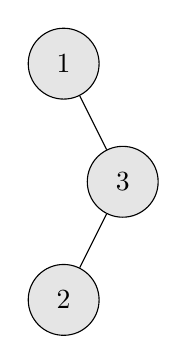
\begin{tikzpicture}
[every node/.style={draw, circle, minimum size=9mm, fill=gray!20!}]
\node{1}
	child[missing]
	child{node{3} child{node{2}} child[missing]};
\end{tikzpicture}
\end{figure}


\textbf{Output}:
1


\textbf{Explanation}:

The minimum absolute difference is 1, which is the difference between 2 and 1 (or between 2 and 3).

\end{flushleft} 

\paragraph{Note:} 
\begin{itemize}
\item There are at least two nodes in this BST.
\end{itemize}
%\section{531 --- Lonely Pixel I}
Given a picture $G$ consisting of black and white pixels, find the number of black lonely pixels.

The picture is represented by a 2D char array consisting of \texttt{B} and \texttt{W}, which means black and white pixels respectively.

A black lonely pixel is character \texttt{B} that located at a specific position where the same row and same column don't have any other black pixels.

\paragraph{Example:}

\begin{flushleft}
\textbf{Input}: 

\begin{table}[H]
\begin{tabular}{ccc}
\texttt{W} & \texttt{W} & \texttt{B}\\
 \texttt{W} & \texttt{B} & \texttt{W}\\
 \texttt{B} & \texttt{W} & \texttt{W}
\end{tabular}
\end{table}


\textbf{Output}: 3

\textbf{Explanation}: All the three \texttt{B}s are black lonely pixels.
\end{flushleft}

\paragraph{Note:}

\begin{itemize}
\item  The range of width and height of the input 2D array is $ [1,500] $.
\end{itemize}

%\section{532 --- K-diff Pairs in an Array}
Given an array of integers $A$ and an integer $ k $, you need to find the number of unique $ k $-diff pairs in the array. Here a $ k $-diff pair is defined as an integer pair $ (i, j) $, where $ i $ and $ j $ are both numbers in the array and their \textbf{absolute difference} is k.

\paragraph{Example 1:}

\begin{flushleft}
\textbf{Input}: $ [3, 1, 4, 1, 5] $, $ k = 2 $

\textbf{Output}: 2

\textbf{Explanation}: 

There are two 2-diff pairs in the array, $ (1, 3) $ and $ (3, 5) $.

Although we have two 1s in the input, we should only return the number of unique pairs.

\end{flushleft}

\paragraph{Example 2:}

\begin{flushleft}
\textbf{Input}:$ [1, 2, 3, 4, 5] $, k = 1

\textbf{Output}: 4

\textbf{Explanation}: There are four 1-diff pairs in the array, $  (1, 2) $, $ (2, 3) $, $ (3, 4) $ and $ (4, 5) $.

\end{flushleft}

\paragraph{Example 3:}
\begin{flushleft}

\textbf{Input}: $ [1, 3, 1, 5, 4] $, $ k = 0 $

\textbf{Output}: 1

\textbf{Explanation}: There is one 0-diff pair in the array, $ (1, 1) $.

\end{flushleft}

\paragraph{Note:}

\begin{itemize}
\item The pairs $(i, j)$ and $(j, i)$ count as the same pair.
\item The length of the array won't exceed 10,000.
\item All the integers in the given input belong to the range: $[-10^7, 10^7]$.
\end{itemize}

%\section{533 --- Lonely Pixel II}
Given a picture $G$ consisting of black and white pixels, and a positive integer $N$, find the number of black pixels located at some specific row \textbf{R} and column \textbf{C} that align with all the following rules:

\begin{itemize}
\item Row R and column C both contain exactly $ N $ black pixels.
\item For all rows that have a black pixel at column \textbf{C}, they should be exactly the same as row \textbf{R}
\end{itemize}

The picture is represented by a 2D char array consisting of \textbf{B} and \textbf{W}, which means black and white pixels respectively.

\paragraph{Example:}

\begin{flushleft}
\textbf{Input}: 
                                           
\begin{table}[H]
\begin{tabular}{cccccc}
W & B & W & B & B & W \\   
W & B & W & B & B & W \\
W & B & W & B & B & W \\
W & W & B & W & B & W
\end{tabular}
\end{table}

$ N = 3 $

\textbf{Output}: 6

\textbf{Explanation}: All the red \textbf{B} are the black pixels we need (all \textbf{B}s at column 1 and 3).

\begin{table}[H]
\begin{tabular}{l|cccccc}
 & 0 &   1&    2 &   3 &   4 &   5 \\
\hline
0 &   W & \textcolor{red}{B} & W & \textcolor{red}{B} & B & W \\    
1  &   W & \textcolor{red}{B} & W & \textcolor{red}{B} & B & W \\    
2  &   W & \textcolor{red}{B} & W & \textcolor{red}{B} & B & W \\    
3  &   W & W & B & W & B & W 
\end{tabular}
\end{table}  

Take \textbf{B} at row $ R = 0 $ and column $ C = 1 $ as an example:

\textbf{Rule 1}: row $ R = 0 $ and column $ C = 1 $ both have exactly $ N = 3 $ black pixels. 

\textbf{Rule 2}, the rows have black pixel at column $ C = 1 $ are row 0, row 1 and row 2. They are exactly the same as row $ R = 0 $.
\end{flushleft}

\paragraph{Note:}

\begin{itemize}
\item  The range of width and height of the input 2D array is $[1,200]$
\end{itemize}.

%\include{534}
%\section{535 --- Encode and Decode TinyURL}
\paragraph{Note:} 
\begin{itemize}
\item This is a companion problem to the \textbf{System Design problem}: \textbf{Design TinyURL}.
\end{itemize}

TinyURL is a URL shortening service where you enter a URL such as \url{https://leetcode.com/problems/design-tinyurl} and it returns a short URL such as \url{http://tinyurl.com/4e9iAk}.

Design the \texttt{encode} and \texttt{decode} methods for the TinyURL service. There is no restriction on how your encode/decode algorithm should work. You just need to ensure that a URL can be encoded to a tiny URL and the tiny URL can be decoded to the original URL.

%\section{536 --- Construct Binary Tree from String}
You need to construct a binary tree from a string consisting of parenthesis and integers.

The whole input represents a binary tree. It contains an integer followed by zero, one or two pairs of parenthesis. The integer represents the root's value and a pair of parenthesis contains a child binary tree with the same structure.

You always start to construct the \textbf{left} child node of the parent first if it exists.

\paragraph{Example:}

\begin{flushleft}
\textbf{Input}: $4(2(3)(1))(6(5))$

\textbf{Output}: return the tree root node representing the following tree:

\begin{figure}[H]
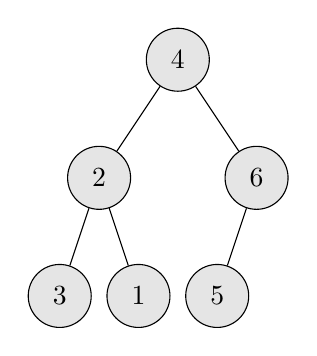
\begin{tikzpicture}
[every node/.style={draw, circle, minimum size=8mm, fill=gray!20},
level 1/.style={sibling distance=20mm},
level 2/.style={sibling distance=10mm}]
\node{4}
 child{ node{2} child {node{3}} child {node{1}}}
 child{ node{6} child {node{5}} child[missing]};
\end{tikzpicture}
\end{figure}


%       4
%     /   \
%    2     6
%   / \   / 
%  3   1 5   

\end{flushleft}

\paragraph{Note:}

\begin{itemize}
\item  There will only be parenthesis, dash and digits in the input string.
\item An empty tree is represented by empty string instead of $()$.
\end{itemize}

%\section{537 --- Complex Number Multiplication}
Given two strings representing two complex numbers.

You need to return a string representing their multiplication. Note $i^2 = -1$ according to the definition.

\paragraph{Example 1:}

\begin{flushleft}
\textbf{Input}: $1+1i$, $1+1i$

\textbf{Output}: $0+2i$

\textbf{Explanation}: $(1 + i) \times (1 + i) = 1 + i^2 + 2 \times i = 2i$, and you need convert it to the form of $0+2i$.

\end{flushleft}

\paragraph{Example 2:}

\begin{flushleft}
\textbf{Input}: $1+-1i$, $1+-1i$

\textbf{Output}: $0+-2i$

\textbf{Explanation}: $(1 - i) \times (1 - i) = 1 + i^2 - 2 \times i = -2i$, and you need convert it to the form of $0+-2i$.
\end{flushleft}

\paragraph{Note:}

\begin{itemize}
\item The input strings will not have extra blank.
\item The input strings will be given in the form of $a+bi$, where the integer $a$ and $b$ will both belong to the range of $[-100, 100]$. And \textbf{the output should be also in this form}.

\end{itemize}
%\section{538 --- Convert BST to Greater Tree}
Given a Binary Search Tree (BST), convert it to a Greater Tree such that every key of the original BST is changed to the original key plus sum of all keys greater than the original key in BST.

\paragraph{Example:}

\begin{flushleft}
\textbf{Input}: The root of a Binary Search Tree like this:

\begin{figure}[H]
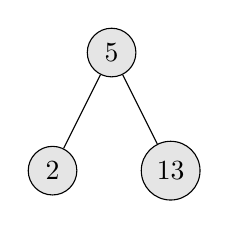
\begin{tikzpicture}
[every node/.style={draw, circle, fill=gray!20!, minimum size=5mm}]

\node{5}
child {node{2}}
child {node{13}};

\end{tikzpicture}
\end{figure}


\textbf{Output}: The root of a Greater Tree like this:

\begin{figure}[H]
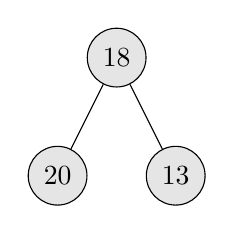
\begin{tikzpicture}
[every node/.style={draw, circle, fill=gray!20!, minimum size=5mm}]

\node{18}
child {node{20}}
child {node{13}};

\end{tikzpicture}
\end{figure}

\end{flushleft}

%\section{539 --- Minimum Time Difference}
Given a list of 24-hour clock time points in \texttt{Hour:Minutes} format, find the \textbf{minimum} minutes difference between any two time points in the list.

\paragraph{Example 1:}

\begin{flushleft}
\textbf{Input}: $[23:59, 00:00]$

\textbf{Output}: 1
\end{flushleft}

\paragraph{Note:}

\begin{itemize}
\item The number of time points in the given list is at least 2 and won't exceed 20000.
\item The input time is legal and ranges from 00:00 to 23:59.
\end{itemize}

%\section{540 --- Single Element in a Sorted Array}
Given a sorted array consisting of only integers where every element appears exactly twice except for one element which appears exactly once. Find this single element that appears only once.


\paragraph{Example 1:}

\begin{flushleft}
\textbf{Input}: $[1,1,2,3,3,4,4,8,8]$

\textbf{Output}: $2$

\end{flushleft}

\paragraph{Example 2:}

\begin{flushleft}
\textbf{Input}: $[3,3,7,7,10,11,11]$

\textbf{Output}: $ 10$
\end{flushleft}

\paragraph{Note:}
\begin{itemize}
    \item Your solution should run in $O(\log n)$ time and $O(1)$ space.
\end{itemize}
%\section{541 --- Reverse String II}
Given a string $s$ and an integer $k$, you need to reverse the first $k$ characters for every $2k$ characters counting from the start of the string. If there are less than $k$ characters left, reverse all of them. If there are less than $2k$ but greater than or equal to $k$ characters, then reverse the first k characters and left the other as original.

\paragraph{Example:}

\begin{flushleft}
\textbf{Input}: $s = \texttt{abcdefg}$, $k = 2$

\textbf{Output}: \texttt{bacdfeg}
\end{flushleft}

\paragraph{Restrictions:}

\begin{itemize}
\item The string consists of lower English letters only.
\item Length of the given string and $k$ will in the range $[1, 10000]$
\end{itemize}

%\section{542 --- 01 Matrix}
Given a matrix consists of 0 and 1, find the distance of the nearest 0 for each cell.

The distance between two adjacent cells is 1.
 

\paragraph{Example 1:}

\begin{flushleft}
\textbf{Input}:
\begin{table}[H]
\begin{tabular}{ccc}
0 & 0 & 0\\
0 & 1 & 0\\
0 & 0 & 0
\end{tabular}
\end{table}


\textbf{Output}:
\begin{table}[H]
\begin{tabular}{ccc}
0 & 0 & 0\\
0 & 1 & 0\\
0 & 0 & 0
\end{tabular}
\end{table}
\end{flushleft}

\paragraph{Example 2:}

\begin{flushleft}
\textbf{Input}:
\begin{table}[H]
\begin{tabular}{ccc}
0 & 0 & 0\\
0 & 1 & 0\\
1 & 1 & 1
\end{tabular}
\end{table}

\textbf{Output}:
\begin{table}[H]
\begin{tabular}{ccc}
0 & 0 & 0\\
0 & 1 & 0\\
1 & 2 & 1
\end{tabular}
\end{table}
\end{flushleft}
 

\paragraph{Note:}

\begin{itemize}
\item The number of elements of the given matrix will not exceed 10,000.
\item There are at least one 0 in the given matrix.
\item The cells are adjacent in only four directions: up, down, left and right.
\end{itemize}


%\section{543 --- Diameter of Binary Tree}
Given a binary tree, you need to compute the length of the diameter of the tree. The diameter of a binary tree is the length of the longest path between any two nodes in a tree. This path may or may not pass through the root.

\paragraph{Example:}
\begin{flushleft}
\textbf{Input}:

\begin{figure}[H]
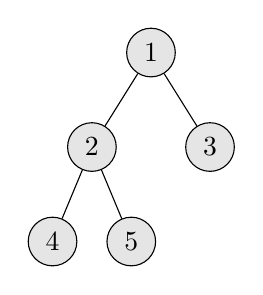
\begin{tikzpicture}
[every node/.style={draw, circle, fill=gray!20!, minimum size=5mm},
level 2/.style ={sibling distance=1cm}, 
level 3/.style={sibling distance=8mm},
level distance=1.2cm]
\node{1}
 child {node{2} child {node{4}} child {node{5}}}
 child {node{3}};
\end{tikzpicture}
\end{figure}

\textbf{Output}: 3, which is the length of the path $[4,2,1,3]$ or $[5,2,1,3]$.
\end{flushleft}
\paragraph{Note:} 
\begin{itemize}
\item The length of path between two nodes is represented by the number of edges between them. 
\end{itemize}
%\section{544 --- Output Contest Matches}
During the NBA playoffs, we always arrange the rather strong team to play with the rather weak team, like make the rank 1 team play with the rank $n$th team, which is a good strategy to make the contest more interesting. Now, you're given $n$ teams, you need to output their \textbf{final} contest matches in the form of a string.

The $n$ teams are given in the form of positive integers from 1 to $n$, which represents their initial rank. (Rank 1 is the strongest team and Rank $n$ is the weakest team.) We'll use parentheses and commas to represent the contest team pairing -- parentheses for pairing and commas for partition. During the pairing process in each round, you always need to follow the strategy of making the rather strong one pair with the rather weak one.

\paragraph{Example 1:}

\begin{flushleft}
\textbf{Input}: 2

\textbf{Output}: $(1,2)$

\textbf{Explanation}:
 
Initially, we have the team 1 and the team 2, placed like: 1,2.

Then we pair the team $(1,2)$ together with parentheses and comma which is the final answer.
\end{flushleft}

\paragraph{Example 2:}

\begin{flushleft}
\textbf{Input}: 4

\textbf{Output}: $((1,4),(2,3))$

\textbf{Explanation}:

In the first round, we pair the team 1 and 4, the team 2 and 3 together, as we need to make the strong team and weak team together.

And we got $(1,4)$, $(2,3)$.

In the second round, the winners of $ (1,4) $ and $ (2,3) $ need to play again to generate the final winner, so you need to add the paratheses outside them.

And we got the final answer $((1,4),(2,3))$.
\end{flushleft}

\paragraph{Example 3:}

\begin{flushleft}
\textbf{Input}: 8

\textbf{Output}: $(((1,8),(4,5)),((2,7),(3,6)))$

\textbf{Explanation}:
 
First round: $(1,8),(2,7),(3,6),(4,5)$

Second round: $((1,8),(4,5)),((2,7),(3,6))$

Third round: $(((1,8),(4,5)),((2,7),(3,6)))$

Since the third round will generate the final winner, you need to output the answer $(((1,8),(4,5)),((2,7),(3,6)))$.
\end{flushleft}

\paragraph{Note:}

\begin{itemize}
\item The $ n $ is in range $[2, 2^{12}]$.
\item We ensure that the input $ n $ can be converted into the form $2^k$, where $k$ is a positive integer.
\end{itemize}
%\section{545 --- Boundary of Binary Tree}
Given a binary tree, return the values of its boundary in \textbf{anti-clockwise} direction starting from root. Boundary includes left boundary, leaves, and right boundary in order \textbf{without duplicate nodes}.  (The values of the nodes may still be duplicates.)

\textbf{Left boundary} is defined as the path from root to the \textbf{left-most} node. \textbf{Right boundary} is defined as the path from root to the \textbf{right-most} node. If the root doesn't have left subtree or right subtree, then the root itself is left boundary or right boundary. Note this definition only applies to the input binary tree, and not applies to any subtrees.

The \textbf{left-most} node is defined as a \textbf{leaf} node you could reach when you always firstly travel to the left subtree if exists. If not, travel to the right subtree. Repeat until you reach a leaf node.

The \textbf{right-most} node is also defined by the same way with left and right exchanged.

\paragraph{Example 1}

\begin{flushleft}
\textbf{Input}:
\begin{figure}[H]
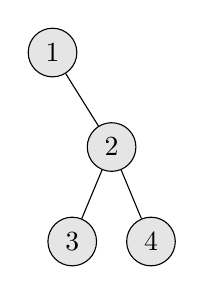
\begin{tikzpicture}
[every node/.style={draw, circle, fill=gray!20!, minimum size=5mm},
level 2/.style ={sibling distance=1cm}, 
level 3/.style={sibling distance=8mm},
level distance=1.2cm]
\node{1}
child[missing]
child{node{2} child{node {3}} child{node{4}}};
\end{tikzpicture}
\end{figure}

\textbf{Output}: $[1, 3, 4, 2]$

\textbf{Explanation}:

The root doesn't have left subtree, so the root itself is left boundary.

The leaves are node 3 and 4.

The right boundary are node 1, 2, 4. Note the anti-clockwise direction means you should output reversed right boundary.

So order them in anti-clockwise without duplicates and we have $[1,3,4,2]$.
\end{flushleft}


\paragraph{Example 2}

\begin{flushleft}
\textbf{Input}:
\begin{figure}[H]
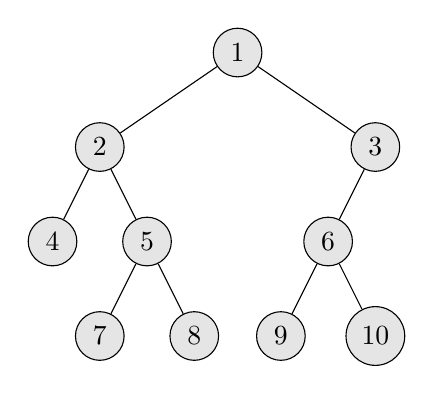
\begin{tikzpicture}
[every node/.style={draw, circle, fill=gray!20!, minimum size=5mm},
level 1/.style ={sibling distance=3.5cm}, 
level 2/.style={sibling distance=2.0cm},
level 2/.style={sibling distance=1.2cm},
level distance=1.2cm]
\node{1}
child{node{2} child{node{4}} child{node{5} child {node{7}} child {node{8}}}}
child{node{3} child{node{6} child{node{9}} child{node{10}}} child[missing]};
\end{tikzpicture}
\end{figure}
      
\textbf{Output}: $[1,2,4,7,8,9,10,6,3]$

\textbf{Explanation}:

The left boundary are node 1, 2, 4. (4 is the left-most node according to definition)

The leaves are node 4, 7, 8, 9, 10.

The right boundary are node 1, 3, 6, 10. (10 is the right-most node).

So order them in anti-clockwise without duplicate nodes we have $[1,2,4,7,8,9,10,6,3]$.
\end{flushleft}

%\section{546 --- Remove Boxes}
Given several boxes with different colors represented by different positive numbers.

You may experience several rounds to remove boxes until there is no box left. Each time you can choose some continuous boxes with the same color (composed of $ k $ boxes, $k \geq 1$), remove them and get $k\times k$ points.
Find the maximum points you can get.

\paragraph{Example 1:}

\begin{flushleft}
\textbf{Input}: $[1, 3, 2, 2, 2, 3, 4, 3, 1]$

\textbf{Output}: 23

\textbf{Explanation}:

$[1, 3, 2, 2, 2, 3, 4, 3, 1] $

$\longrightarrow [1, 3, 3, 4, 3, 1]$ ($3\times 3=9$ points)

$\longrightarrow [1, 3, 3, 3, 1]$ ($1\times 1=1$ points)

$\longrightarrow [1,1]$ ($3\times 3=9$ points)

$\longrightarrow []$ ($2\times 2=4$ points)
\end{flushleft}

\paragraph{Note:} 
\begin{itemize}
\item The number of boxes $n$ would not exceed 100.
\end{itemize}

%\section{547 --- Friend Circles}
There are $ N $ students in a class. Some of them are friends, while some are not. Their friendship is transitive in nature. For example, if $ A $ is a direct friend of $ B $, and $ B $ is a direct friend of $ C $, then $ A $ is an indirect friend of $ C $. And we defined a friend circle is a group of students who are direct or indirect friends.

Given a $N\times N$ matrix $ M $ representing the friend relationship between students in the class. If $M[i][j] = 1$, then the $i$th and $j$th students are direct friends with each other, otherwise not. And you have to output the total number of friend circles among all the students.

\paragraph{Example 1:}
\begin{flushleft}

\textbf{Input}:
\begin{table}[H]
\begin{tabular}{ccc}
1 & 1 & 0\\
1 & 1 & 0\\
0 & 0 & 1
\end{tabular}
\end{table} 

\textbf{Output}: 2

\textbf{Explanation}:

The 0th and 1st students are direct friends, so they are in a friend circle. 

The 2nd student himself is in a friend circle. So return 2.
\end{flushleft}

\paragraph{Example 2:}
\begin{flushleft}

\textbf{Input}:
\begin{table}[H]
\begin{tabular}{ccc}
1 & 1 & 0\\
1 & 1 & 1\\
0 & 1 & 1
\end{tabular}
\end{table} 

\textbf{Output}: 1

\textbf{Explanation}:

The 0th and 1st students are direct friends, the 1st and 2nd students are direct friends, 

so the 0th and 2nd students are indirect friends. All of them are in the same friend circle, so return 1.
\end{flushleft}

\paragraph{Note:}
\begin{itemize}
\item $N$ is in range $[1,200]$.
\item $M[i][i] = 1$ for all students.
\item If $M[i][j] = 1$, then $M[j][i] = 1$.
\end{itemize}

\subsection{DFS}
\begin{itemize}
\item The given matrix can be viewed as the Adjacency Matrix of a graph. By viewing the matrix in such a manner, our problem reduces to the problem of finding the number of connected components in an undirected graph.
\item In order to find the number of connected components in an undirected graph, one of the simplest methods is to make use of \textbf{Depth First Search} starting from every node. We make use of an array of size $N\times N$, $V$, to indicate that the $i^{\texttt{th}}$ node has already been visited while undergoing a \textbf{Depth First Search} from some node.
\item To undergo DFS, we pick up a node and visit all its directly connected nodes. But, as soon as we visit any of those nodes, we recursively apply the same process to them as well. Thus, we try to go as deeper into the levels of the graph as possible starting from a current node first, leaving the other direct neighbour nodes to be visited later on.
\end{itemize}

\setcounter{lstlisting}{0}
\begin{lstlisting}[style=customc, caption={DFS}]
int findCircleNum( vector<vector<int>>& M )
{
    auto N = static_cast<int>( M.size() );

    vector<int> seen( N, 0 );

    int ans = 0;

    //test each person
    for( int i = 0; i < N; ++i )
    {
        if( seen[i] == 0 )
        {
            //person i has not been
            //visited, dfs from him
            dfs( M, i, seen );
            ++ans;
        }
    }

    return ans;
}

//depth first search
void dfs( vector<vector<int>>& M, int x, vector<int>& seen )
{
    auto N = static_cast<int>( M.size() );

    for( int y = 0; y < N; ++y )
    {
        if( ( M[x][y] == 1 ) && ( seen[y] == 0 ) )
        {
            //y is the friend of x
            //and y has not been visited
            seen[y] = 1;
            dfs( M, y, seen );
        }
    }
}
\end{lstlisting}

\subsection{BFS}
\begin{itemize}
\item In case of \textbf{Breadth First Search}, we start from a particular node and visit all its directly connected nodes first. After all the direct neighbours have been visited, we apply the same process to the neighbour nodes as well. Thus, we exhaust the nodes of a graph on a level by level basis.
\item We also make use of an array, $V$, to keep a track of the already visited nodes. We increment the count of connected components whenever we need to start off with a new node as the root node for applying BFS which hasn't been already visited.
\end{itemize}

\setcounter{lstlisting}{0}
\begin{lstlisting}[style=customc, caption={BFS}]
int findCircleNum( vector<vector<int>>& M )
{
    int N = static_cast<int>( M.size() );

    queue<int> q;

    vector<int> seen( N, 0 );

    int ans = 0;

    for( int i = 0; i < N; ++i )
    {
        if( seen[i] == 0 )
        {
            //for each unvisited persion
            //we apply BFS from this person
            //q will be reused
            q.push( i );

            while( !q.empty() )
            {
                auto x = q.front();
                q.pop();

                seen[x] = 1;

                for( int y = 0; y < N; ++y )
                {
                    if( ( M[x][y] == 1 ) && ( seen[y] == 0 ) )
                    {
                        //y is friend of x
                        //and has not been visited
                        q.push( y );
                    }
                }
            }

            ++ans;
        }
    }

    return ans;
}
\end{lstlisting}

\subsection{Union Find}
\begin{itemize}
\item Another method that can be used to determine the number of connected components in a graph is the \textbf{union find} method.
\item We make use of an array of size $N$, $P$. We traverse over all the nodes of the graph. For every node traversed, we traverse over all the nodes directly connected to it and assign them to a single group which is represented by their parent node. This process is called forming a union. Every group has a single parent node.
\item For every new pair of nodes found, we look for the parents of both the nodes. If the parents nodes are the same, it indicates that they have already been united into the same group. If the parent nodes differ, it means they are yet to be united. Thus, for the pair of nodes $ (x, y) $, while forming the union, we assign $P[P[y]] \gets P[x]$, which ultimately combines them into the same group.
\end{itemize}

\setcounter{lstlisting}{0}
\begin{lstlisting}[style=customc, caption={Union Find}]
int findCircleNum( vector<vector<int>>& M )
{
    auto N = static_cast<int>( M.size() );

    vector<int> parents( N, 0 );

    for( int i = 1; i <= N; ++i )
    {
        parents[i - 1] = i - 1;
    }

    for( int r = 0; r < N; ++r )
    {
        for( int c = 0; c < N; ++c )
        {
            if( M[r][c] == 1 )
            {
                //put r and c into one
                //parent
                group( parents, r, c );
            }
        }

    }

    int ans = 0;

    for( int i = 1; i <= N; ++i )
    {
        if( parents[i - 1] == i - 1 )
        {
            //each group's parent
            //is the parent itself
            ++ans;
        }
    }

    return ans;
}

//union x and y
void group( vector<int>& parents, int x, int y )
{
    int px = find_parent( parents, x );
    int py = find_parent( parents, y );

    if( px != py )
    {
        parents[py] = px;
    }
}

//find parent of x
int find_parent( vector<int>& parents, int x )
{
    while( parents[x] != x )
    {
        x = parents[x];
    }

    return x;
}
\end{lstlisting}
%\section{548 --- Split Array with Equal Sum}
Given an array with $n$ integers, $A$, you need to find if there are triplets $(i, j, k)$ which satisfies following conditions:

\begin{itemize}
\item$ 0 < i, i + 1 < j$, $j + 1 < k < n - 1$
\item Sum of subarrays $(0, i - 1)$, $ (i + 1, j - 1) $, $(j + 1, k - 1)$ and $(k + 1, n - 1)$ should be equal.
\end{itemize}

where we define that subarray $ (L, R) $ represents a slice of the original array starting from the element indexed $L$ to the element indexed $R$.

\paragraph{Example:}

\begin{flushleft}
\textbf{Input}: $[1,2,1,2,1,2,1]$

\textbf{Output}: \texttt{True}

\textbf{Explanation}:

$i = 1, j = 3, k = 5$.

$\sum A(0, i - 1) = \sum A(0, 0) = 1$

$\sum A(i + 1, j - 1) = \sum A(2, 2) = 1$

$\sum A(j + 1, k - 1) = \sum A(4, 4) = 1$

$\sum A(k + 1, n - 1) = \sum A(6, 6) = 1$
\end{flushleft}

\paragraph{Note:}

\begin{itemize}
\item $1 \leq n \leq 2000$
\item Elements in the given array will be in range $[-1,000,000, 1,000,000]$.
\end{itemize}

\subsection{Hash Map and Mathematical Induction}
\begin{itemize}
\item From the given condition, we can get $i\geq 1$, $j \geq 3$ and $k\geq 5$, and the length of the array must be no less than 7.
\item Create a prefix summation array $P$ with same length as the input array.
\item From the given condition, we can get the following equations
\begin{align*}
P[j-1] - P[i] &= P[i-1] \\
P[k-1] - P[j] &= P[j-1] - P[i]\\
P[n-1] - P[k] &= P[k-1] - P[j]\\
\end{align*}
By arrange these equations we can get
\begin{align*}
P[j-1] &=  P[i] + P[i-1] \\
P[k-1] + P[i] &= P[j] + P[j-1]\\
P[n-1] + P[j] &= P[k] + P[k-1]\\
\end{align*}
As we can see, $P[x]+P[x-1]$ is the important characteristic.
\item Therefore, create a hash map with the key equal to $P[x] + P[x-1]$ and the value is the array of associated indexes.
\item From $j=3$ until $n-4$, we try each $j$
 \begin{enumerate}
 \item Find in the hash map if any key equal to $P[j-1]$. If there is a key equal to $P[j-1]$, there exists some $i$ that $P[i] + P[i-1] = P[j-1]$ (the first equation). We must make sure that $i+1 < j$ by the given condition. Since the array of associated indexes are sorted, we can use a binary search to find the candidates of $i$ in the array
 \item Then we find if any key equal to $P[n-1]+P[j]$. If there is a key equal to $P[n-1]+P[j]$, there exists some $k$ that $P[n-1] + P[j] = P[k] + P[k-1]$ (the third equation). We must make sure that $j+1<k$ by the given condition. Similarly, we use a binary search to find the candidates $k$ in the array.
 \item Finally, we need to traverse each $i$ and $k$ to make sure that $P[k-1] + P[i] = P[j] + P[j-1]$ (the second equation)
 \end{enumerate}
\end{itemize}

\setcounter{lstlisting}{0}
\begin{lstlisting}[style=customc, caption={Hash Map}]
bool splitArray( vector<int>& nums )
{

    //i>=1, j>=3, k>=5, n>=7
    if( nums.empty() || ( nums.size() < 7 ) )
    {
        return false;
    }

    vector<int> ps( nums.size(), 0 );
    ps[0] = nums[0];

    unordered_map<int, vector<int>> m;

    int L = static_cast<int>( nums.size() );

    //get prefix sum
    //create the hash map with key equal to
    //ps[i]+ps[i-1] and associated indexes
    for( int i = 1; i < L; ++i )
    {
        ps[i] = ps[i - 1] + nums[i];

        auto it = m.find( ps[i] + ps[i - 1] );
        if( it == m.end() )
        {
            m.emplace( ps[i] + ps[i - 1], vector<int> {i} );
        }
        else
        {
            it->second.push_back( i );
        }
    }


    //test each j to find
    //if there exists i and k
    for( int j = 3 ; j < L - 3; ++j )
    {
        //i and j must satisfy
        //ps[j-1] = ps[i] + ps[i-1]
        auto it = m.find( ps[j - 1] );
        if( it == m.end() )
        {
            continue;
        }

        //find first index that is
        //no less than j-1;
        //then it->second[0,x] is the candidiates of i
        int x = leftmost( it->second, j - 1 );

        //j and k must satisfy
        //ps[j] + ps[n-1] = ps[k] + ps[k-1]
        auto it_k = m.find( ps[j] + ps.back() );
        if( it_k == m.end() )
        {
            continue;
        }


        //find the first index that is
        //larger than j+1 (k)
        //then it_k->second[y,len-1] is the candidates of k
        int y = rightmost( it_k->second, j + 1 );
        int len = static_cast<int>( it_k->second.size() );

        //i,j and k must satisfy
        //ps[i] + ps[k-1] = ps[j] + ps[j-1]
        int z = ps[j] + ps[j - 1];

        for( int u = 0; u < x; ++u )
        {
            int i = it->second[u];

            for( int v = y; v < len; ++v )
            {
                int k = it_k->second[v];

                if( ps[k - 1] + ps[i] == z )
                {
                    return true;
                }
            }
        }
    }

    return false;
}

int leftmost( vector<int>& A, int target )
{
    int l = 0;
    int r = static_cast<int>( A.size() );

    while( l < r )
    {
        int mid = ( l + r ) / 2;
        if( A[mid] < target )
        {
            l = mid + 1;
        }
        else
        {
            r = mid;
        }
    }

    return l;
}

int rightmost( vector<int>& A, int target )
{
    int l = 0;
    int r = static_cast<int>( A.size() );

    while( l < r )
    {
        int mid = ( l + r ) / 2;
        if( A[mid] <= target )
        {
            l = mid + 1;
        }
        else
        {
            r = mid;
        }
    }

    return l;
}
\end{lstlisting}
\section{549 --- Binary Tree Longest Consecutive Sequence II}
Given a binary tree, you need to find the length of Longest Consecutive Path in Binary Tree.

Especially, this path can be either increasing or decreasing. For example, $ [1,2,3,4] $ and $ [4,3,2,1] $ are both considered valid, but the path $ [1,2,4,3] $ is not valid. On the other hand, the path can be in the child-Parent-child order, where not necessarily be parent-child order.

\paragraph{Example 1:}
\begin{flushleft}

\textbf{Input}:
\begin{figure}[H]
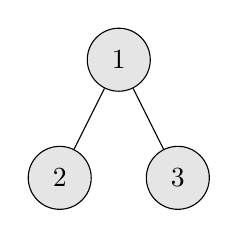
\begin{tikzpicture}
[every node/.style={draw, circle, minimum size=8mm, fill=gray!20!}]
\node{1}
child{node{2}}
child{node{3}};
\end{tikzpicture}
\end{figure}
\textbf{Output}: 2

\textbf{Explanation}: The longest consecutive path is $[1, 2]$ or $[2, 1]$.
 

\end{flushleft}

\paragraph{Example 2:}
\begin{flushleft}
\textbf{Input}:
\begin{figure}[H]
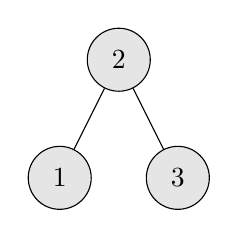
\begin{tikzpicture}
[every node/.style={draw, circle, minimum size=8mm, fill=gray!20!}]
\node{2}
child{node{1}}
child{node{3}};
\end{tikzpicture}
\end{figure}


\textbf{Output}: 3

\textbf{Explanation}: The longest consecutive path is $ [1, 2, 3] $ or $ [3, 2, 1] $.
\end{flushleft}
 

\paragraph{Note:} 
\begin{itemize}
\item All the values of tree nodes are in the range of $[-10^{7}, 10^{7}]$.
\end{itemize}

\subsection{Single Traversal}
\begin{itemize}
\item With every node, we associate two values named $x$ and $y$, where $x$ represents the length of the longest increment branch below the current node including itself, and $y$ represents the length of the longest decrement branch below the current node including itself.
\item We start off by assigning both $x$ and $y$ as 1 for the current node. This is because the node itself always forms a consecutive increasing as well as decreasing path of length 1.
\item Then, we obtain the length of the longest path for the left child of the current node recursively. Now, if the left child is less than the current node, it forms a decreasing sequence with the current node. Thus, the $y$ value for the current node is stored as the left child's $y$ value plus 1. But, if the left child is larger than the current node, it forms an increment sequence with the current node. Thus, we update the current node's $x$ value as left child's $x$ value plus 1.
\item Then, we do the same process with the right child as well. But, for obtaining the $x$ and $y$ value for the current node, we need to consider the maximum value out of the two values obtained from the left and the right child for both $x$ and $y$ since we need to consider the longest sequence possible.
\item After we've obtained the final updated values of $x$ and $y$ for a node, we update the length of the longest consecutive path found so far, $\ell$, as $\max(\ell, x+y-1)$.
\end{itemize}

\setcounter{lstlisting}{0}
\begin{lstlisting}[style=customc, caption={DFS}]
int longestConsecutive( TreeNode* root )
{
    if( !root )
    {
        return 0;
    }

    int x = 1;
    int y = 1;

    int best = 0;

    dfs( root, x, y, best );

    return best;
}

//x: the length of longest
//   incrementing sequence length below of current node
//   including current node
//y: the length of longest
//   decrementing sequence length blow of current node
//   inlcluding the current node
void dfs( TreeNode* node, int& x,  int &y, int& best )
{
    if( !node )
    {
        return;
    }

    int lx = 0;
    int ly = 0;

    if( node->left )
    {
        lx = 1;
        ly = 1;

        dfs( node->left, lx, ly, best );

        if( node->left->val == node->val - 1 )
        {
            //current node and left node
            //form a incrementing pair
            x = lx + 1;
        }
        else if( node->left->val == node->val + 1 )
        {
            //current node and left node
            //form a decrementing pair
            y = ly + 1;
        }
    }

    int rx = 0;
    int ry = 0;

    if( node->right )
    {
        rx = 1;
        ry = 1;

        dfs( node->right, rx, ry, best );

        if( node->right->val == node->val - 1 )
        {
            //current node and right node
            //form a incrementing pair
            //we need maximum one
            x = ( max )( x, rx + 1 );
        }
        else if( node->right->val == node->val + 1 )
        {
            //current node and right node
            //form a decrementing pair
            //we need maximum one
            y = ( max )( y, ry + 1 );
        }
    }

    best = ( max )( best, x + y - 1 );
}
\end{lstlisting}
%\include{550}
%\include{551}
%\section{552 --- Student Attendance Record II}
Given a positive integer $n$, return the number of all possible attendance records with length $n$, which will be regarded as rewardable. The answer may be very large, return it after mod $10^9 + 7$.

A student attendance record is a string that only contains the following three characters:

\begin{itemize}
\item \texttt{A} : Absent.
\item \texttt{L} : Late.
\item \texttt{P} : Present.
\end{itemize}

A record is regarded as rewardable if it doesn't contain more than one \texttt{A} (absent) or more than two continuous \texttt{L} (late).

\paragraph{Example 1:}

\begin{flushleft}
\textbf{Input}: $n = 2$

\textbf{Output}: 8 

\textbf{Explanation}:

There are 8 records with length 2 will be regarded as rewardable:

\texttt{PP}, \texttt{AP}, \texttt{PA}, \texttt{LP}, \texttt{PL}, \texttt{AL}, \texttt{LA}, \texttt{LL}

Only \texttt{AA} won't be regarded as rewardable owing to more than one absent times. 
\end{flushleft}

\paragraph{Note:} 
\begin{itemize}
\item The value of $n$ won't exceed 100,000.
\end{itemize}

\subsection{Dynamic Programming}
\begin{itemize}
\item We can divide the current available rewardable strings with length $\ell$ into following categories
\begin{enumerate}
\item End with one \texttt{A}. No any other \texttt{A} in the string. Denote number of this kind of string as $x$.
\item End with \texttt{L} without \texttt{A}. Denote number of this kind of string as $y_0$
\item End with \texttt{L} with only one \texttt{A}. Denote number of this kind of string as $y_1$
\item End with \texttt{P} without \texttt{A}. Denote number of this kind of string as $z_0$
\item End with \texttt{P} with only one \texttt{A}. Denote number of this kind of string as $z_1$
\item End with \texttt{LL} without \texttt{A}. Denote number of this kind of string as $t_0$
\item End with \texttt{LL} with only one \texttt{A}. Denote number of this kind of string as $t_1$
\end{enumerate}
\item Then for the rewardable strings with length $\ell+1$, we can get the following relationship
\begin{enumerate}
\item To get type 1, we can't add anymore \texttt{A}. We can only add \texttt{A} to type 2, 4 and 6. As such, the number of type 1 string with length $\ell+1$, $\hat{x}$, depends on $y_0$, $z_0$ and $t_0$, i.e., $\hat{x}:=y_0+z_0+t_0$.
\item To get type 2, this type of string cannot have any \texttt{A}. Since this type of string is ending with only one \texttt{L}, We can only add \texttt{L} to type 4. Hence, the number of type 2 string with length $\ell+1$, $\hat{y}_0$, only depends on $z_0$, i.e., $\hat{y}_0:=z_0$
\item To get type 3, this type of string has only one \texttt{A}. We can only add \texttt{L} to type 1 and 5. Similarly, we have $\hat{y}_1:=x+z_1$.
\item To get type 4, we can add \texttt{L} or \texttt{P} to type 2, 4 and 6, except \texttt{A}. $\hat{z}_0:= y_0+z_0+t_0$.
\item To get type 5, we can add \texttt{P} to type 1, 3, 5 and 7. $\hat{z}_1:=x + y_1 + z_1 + t_1$
\item To get type 6, we can add \texttt{L} to type 2. $\hat{t}_0:=y_0$.
\item To get type 7, we can add \texttt{L} to type 3. $\hat{t}_1:=y_1$.
\end{enumerate}
\end{itemize}

\setcounter{lstlisting}{0}
\begin{lstlisting}[style=customc, caption={Dynamic Programming}]
int checkRecord( int n )
{
    int x = 1; //end with A

    int y0 = 1; //end with L without A
    int y1 = 0; //end with L with 1 A

    int z0 = 1; //end with P without A
    int z1 = 0; //end with P with 1 A

    int t0 = 0; //end with LL without A
    int t1 = 0; //end with LL with 1 A

    auto bmod = []( int n )
    {
        return n % ( 1000000007 );
    };

    for( int i = 2; i <= n; ++i )
    {
        int last_x = x;

        int last_y0 = y0;
        int last_y1 = y1;

        int last_z0 = z0;
        int last_z1 = z1;

        int last_t0 = t0;
        int last_t1 = t1;

        x = bmod( bmod( last_y0 + last_z0 ) + last_t0 ); //type 1

        y0 = last_z0; //type 2
        y1 = bmod( last_x + last_z1 ); //type 3

        z0 = bmod( bmod( last_y0 + last_z0 ) + last_t0 ); //type 4
        z1 = bmod( bmod( last_x + last_y1 ) + bmod( last_z1 + last_t1 ) ); //type 5

        t0 = last_y0; //type 6
        t1 = last_y1; //type 7
    }

    //the total of seven types is the answer
    return bmod( bmod( bmod( x + y0 ) + bmod( z0 + t0 ) ) + bmod( bmod( y1 + z1 ) + t1 ) );

}
\end{lstlisting}
%\section{553 --- Optimal Division}
Given a list of \textbf{positive integers} $A$, the adjacent integers will perform the float division. For example, $[2,3,4] \longrightarrow 2 / 3 / 4$.

However, you can add any number of parenthesis at any position to change the priority of operations. You should find out how to add parenthesis to get the maximum result, and return the corresponding expression in string format. \textbf{Your expression should NOT contain redundant parenthesis}.

\paragraph{Example:}
\begin{flushleft}
\textbf{Input}: $[1000,100,10,2]$

\textbf{Output}: $1000/(100/10/2)$

\textbf{Explanation}:

$1000/(100/10/2) = 1000/((100/10)/2) = 200$

However, the bold parenthesis in $1000/((100/10)/2)$ are redundant, since they don't influence the operation priority. So you should return $1000/(100/10/2)$. 

Other cases:

$1000/(100/10)/2 = 50$

$1000/(100/(10/2)) = 50$

$1000/100/10/2 = 0.5$

$1000/100/(10/2) = 2$
\end{flushleft}

\paragraph{Note:}

\begin{itemize}
\item The length of the input array is $[1, 10]$.
\item Elements in the given array will be in range $[2, 1000]$.
\item There is only one optimal division for each test case.
\end{itemize}

%\section{554 -- Brick Wall}

There is a brick wall in front of you. The wall is rectangular and has several rows of bricks. The bricks have the same height but different width. You want to draw a vertical line from the top to the bottom and cross the least bricks.

The brick wall is represented by a list of rows. Each row is a list of integers representing the width of each brick in this row from left to right.

If your line go through the edge of a brick, then the brick is not considered as crossed. You need to find out how to draw the line to cross the least bricks and return the number of crossed bricks.

You cannot draw a line just along one of the two vertical edges of the wall, in which case the line will obviously cross no bricks.

 

\paragraph{Example:}


\begin{flushleft}
\textbf{Input}: 

\begin{table}[H]
\begin{tabular}{cccc}
1 & 2 & 2 & 1\\
3 & 1 & 2 & \\
1 & 3 & 2 & \\
2 & 4 &  & \\
3 & 1 & 2 & \\
1 & 3 & 1 & 1
\end{tabular}
\end{table}

\textbf{Output}: 2

\textbf{Explanation}: 

\begin{figure}[H]
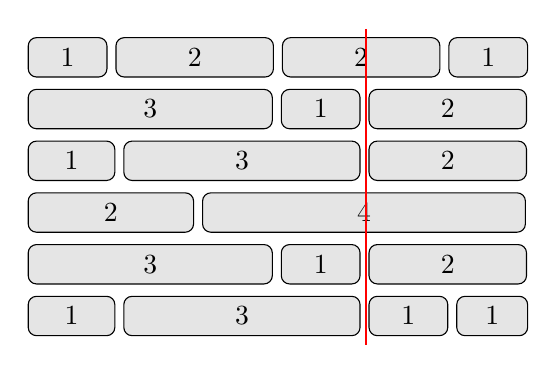
\begin{tikzpicture}
[every node/.style={draw, rectangle, fill=gray!20!, rounded corners=3pt, minimum height=5mm},
node distance=1mm]
\node(0)[minimum width=1cm]{1};
\node(1)[right=of 0, minimum width=2cm] {2};
\node(2)[right=of 1, minimum width=2cm] {2};
\node(3)[right=of 2, minimum width=1cm] {1};
\node(10)[below=4mm of 0.south west, minimum width=3.1cm, anchor=west] {3};
\node(11)[right=of 10, minimum width=1cm, anchor=west] {1};
\node(12)[right=of 11, minimum width=2cm, anchor=west] {2};
\node(20)[below=4mm of 10.south west, minimum width=1.1cm, anchor=west] {1};
\node(21)[right=of 20, minimum width=3cm, anchor=west] {3};
\node(22)[right=of 21, minimum width=2cm, anchor=west] {2};

\node(30)[below=4mm of 20.south west, minimum width=2.1cm, anchor=west] {2};
\node(31)[right=of 30, minimum width=4.1cm, anchor=west] {4};

\node(40)[below=4mm of 30.south west, minimum width=3.1cm, anchor=west] {3};
\node(41)[right=of 40, minimum width=1cm, anchor=west] {1};
\node(42)[right=of 41, minimum width=2cm, anchor=west] {2};

\node(50)[below=4mm of 40.south west, minimum width=1.1cm, anchor=west] {1};
\node(51)[right=of 50, minimum width=3cm, anchor=west] {3};
\node(52)[right=of 51, minimum width=1cm, anchor=west] {1};
\node(53)[right=of 52, minimum width=0.9cm, anchor=west] {1};
\coordinate (p1) at ($(51.south east |- 2.north)+(2pt,3pt)$);
\coordinate (p2) at ($(51.south east)+(2pt,-3pt)$);
%\draw[thick, color=red]  -- $(51.south east)+(3pt, 3pt)$;
\draw[thick, color=red] (p1) -- (p2);
\end{tikzpicture}
\end{figure}
\end{flushleft}

 

\paragraph{Note:}

\begin{itemize}
\item The width sum of bricks in different rows are the same and won't overflow integer type.
\item The number of bricks in each row is in range $[1,10,000]$. The height of wall is in range $[1,10,000]$. Total number of bricks of the wall won't exceed 20,000.
\end{itemize}

%\section{555 --- Split Concatenated Strings}
Given a list of strings, $A$, you could concatenate these strings together into a loop, where for each string you could choose to reverse it or not. Among all the possible loops, you need to find the \textbf{lexicographically biggest} string after cutting the loop, which will make the looped string into a regular one.

Specifically, to find the lexicographically biggest string, you need to experience two phases:

\begin{itemize}
\item Concatenate all the strings into a loop, where you can reverse some strings or not and connect them in the same order as given.
\item Cut and make one breakpoint in any place of the loop, which will make the looped string into a regular one starting from the character at the cutpoint.
\end{itemize}

And your job is to find the lexicographically biggest one among all the possible regular strings.

\paragraph{Example:}

\begin{flushleft}
\textbf{Input}: \texttt{abc}, \texttt{xyz}

\textbf{Output}: \texttt{zyxcba}

Explanation: 

You can get the looped string -\texttt{abcxyz}-, -\texttt{abczyx}-, -\texttt{cbaxyz}-, -\texttt{cbazyx}-, 

where dash represents the looped status. 

The answer string came from the fourth looped one, 

where you could cut from the middle character \texttt{a} and get \texttt{zyxcba}.
\end{flushleft}

\paragraph{Note:}

\begin{itemize}
\item The input strings will only contain lowercase letters.
\item The total length of all the strings will not over 1,000.
\end{itemize}

\subsection{Analysis}
\begin{itemize}
\item Per the description of the problem, the relative ordering of the input strings doesn't change after applying the transformations(i.e. reversing and applying cuts).
\item Consider a given list of strings: $[s_1,s_2,s_3,\ldots,s_j,\ldots, s_n]$. Assuming that we choose $s_j$​ to be the string on which the current cut is placed leading to the formation of two substrings from $s_j$, say $\alpha$ and $\beta$. Thus, the concatenated string formed by such a cut will be: $[\beta,s_{j+1},\ldots,s_n,\hat{s}_1,\hat{s}_2,\ldots,\hat{\alpha}]$. Here, $\hat{s}_i$​ means the reversed $s_i$.
\item We can try each index as a cut in $s_j$, the lexicographically largest concatenated string will be given by: $[\beta,\max(s_{j+1},\hat{s}_{j+1}),\ldots,\max(s_{n},\hat{s}_{n}),\max(s_{1},\hat{s}_{1}),\ldots,\hat{\alpha}]$.
\item Thus, if a particular string $s_j$ is finalized for the cut, the largest lexicographic concatenated string is dependent only on whether the string $s_j$​ is reversed or not, and also on the position of the cut. This happens because the reverse/not reverse operation for the rest of the strings is fixed for a chosen $s_j$​ as shown above and thus, doesn't impact the final result.
\item Then, the algorithm is clear. 
\begin{enumerate}
\item For every given string, we replace the string with the lexicographically larger string from the original string and the reversed one. 
\item Later, we test every string(chosen as the string on which the cuts will be applied), and apply a cut at all the positions of this one and form the full concatenate string keeping the other strings intact. We also test the reversed current string and follow the same process. While doing this, we keep track of the largest lexicographic string found so far.
\end{enumerate}
\end{itemize}

\setcounter{lstlisting}{0}
\begin{lstlisting}[style=customc, caption={Test Cuts}]
string splitLoopedString( vector<string>& strs )
{
    //generate larger string comparing
    //reversed one and original string.
    for( auto& s : strs )
    {
        auto r = s;
        reverse( begin( r ), end( r ) );
        if( r > s )
        {
            s = r;
        }
    }

    string suffix;
    string prefix;

    string ans;
    for( size_t i = 0; i < strs.size(); ++i )
    {
        auto& s = strs[i];

        auto r = s;

        reverse( begin( r ), end( r ) );

        suffix.clear();
        prefix.clear();

        //all the other strings are
        //remained as they are

        //suffix are append to current string's
        //right part
        for( size_t j = i + 1; j < strs.size(); ++j )
        {
            suffix += strs[j];
        }

        //prefix are append to current string's
        //left part
        for( size_t j = 0; j < i; ++j )
        {
            prefix += strs[j];
        }

        for( size_t si = 0; si < s.size(); ++si )
        {
            //test cut on each index si
            //substr(si) get the right part
            string t = s.substr( si );
            string rt = r.substr( si );

            t += suffix;
            t += prefix;

            rt += suffix;
            rt += prefix;

            if( si > 0 )
            {
                //substr(0, si) get the left part
                t += s.substr( 0, si );
                rt += r.substr( 0, si );
            }

            if( ans.empty() )
            {
                ans = t;
            }
            else
            {
                ans = ( max )( ans, t );
            }

            ans = ( max )( ans, rt );

        }
    }

    return ans;
}
\end{lstlisting}

%\section{556 --- Next Greater Element III}
Given a positive 32-bit integer $n$, you need to find the smallest 32-bit integer which has exactly the same digits existing in the integer $n$ and is greater in value than $n$. If no such positive 32-bit integer exists, you need to return $-1$.

\paragraph{Example 1:}

\begin{flushleft}
\textbf{Input}: $12$

\textbf{Output}: $21$
\end{flushleft}

 

\paragraph{Example 2:}

\begin{flushleft}
\textbf{Input}: $21$

\textbf{Output}: $-1$
\end{flushleft}

\subsection{Next Permutation}

The following algorithm generates the next permutation lexicographically after a given permutation $A$. It changes the given permutation in-place.

\begin{enumerate}
\item Find the largest index $k$ such that $A[k] < A[k + 1]$. If no such index exists, the permutation is the last (largest) permutation.
\item Find the largest index $x$ greater than k such that $A[k] < A[x]$.
\item Swap the value of $A[k]$ with that of $A[l]$.
\item Reverse the sequence from $A[k + 1]$ up to and including the final element $A[L-1]$.
\end{enumerate}

For example, given the sequence $A = [1, 2, 3, 4]$ (which is in increasing order), and given that the index is zero-based, the steps are as follows:

\begin{itemize}
\item Index $k = 2$, because 3 is placed at an index that satisfies condition of being the largest index that is still less than $A[k + 1]$ which is 4.
\item Index $x = 3$, because 4 is the only value in the sequence that is greater than 3 in order to satisfy the condition $A[k] < A[x]$.
\item The values of $A[2]$ and $A[3]$ are swapped to form the new sequence $[1,2,4,3]$.
\item The sequence after $k$-index $A[2]$ to the final element is reversed. Because only one value lies after this index (the 3), the sequence remains unchanged in this instance. Thus the lexicographic successor of the initial state is permuted: $[1,2,4,3]$.
\end{itemize}

\setcounter{lstlisting}{0}
\begin{lstlisting}[style=customc, caption={Next Permutation}]
int nextGreaterElement( int n )
{
    vector<int> digits;

    int t = n;
    while( n )
    {
        int q = n / 10;
        int r = n - q * 10;

        digits.push_back( r );

        n = q;
    }

    //make sure the digits of n
    //are from high to low positions
    reverse( begin( digits ), end( digits ) );

    int L = static_cast<int>( digits.size() );

    int i = L - 2;
    bool flag = false;
    //find first k so that A[k] < A[k+1]
    for( i = L - 2; i >= 0; --i )
    {
        if( digits[i + 1] > digits[i] )
        {
            flag = true;
            break;
        }
    }

    if( !flag )
    {
        //n is already the largest one
        return -1;
    }

    int j = L - 1;
    //find largest x ( x > i)
    //so that A[x] > A[k]
    for( ; j > i; --j )
    {
        if( digits[j] > digits[i] )
        {
            break;
        }
    }

    //swap A[x] and A[i]
    swap( digits[j], digits[i] );

    //reverse A[k+1] to A[L-1]
    reverse( digits.begin() + i + 1, digits.end() );

    int ans = 0;

    int max_limit = INT_MAX / 10;

    auto is_overflow = [max_limit]( int n, int d ) -> bool
    {
        if( n > max_limit )
        {
            return true;
        }

        if( ( n == max_limit ) && ( d > 7 ) )
        {
            return true;
        }

        return false;
    };

    for( int d : digits )
    {
        //we need to check integer type
        //overflow
        if( is_overflow( ans, d ) )
        {
            return -1;
        }

        ans = ans * 10 + d;
    }

    return ans;
}
\end{lstlisting}
%\section{557 --- Reverse Words in a String III}
Given a string, you need to reverse the order of characters in each word within a sentence while still preserving whitespace and initial word order.

\paragraph{Example 1:}

\begin{flushleft}

\textbf{Input}: \texttt{Let's take LeetCode contest}

\textbf{Output}: \texttt{s'teL ekat edoCteeL tsetnoc}

\end{flushleft}

%\paragraph{Note:} 
%\begin{itemize}
%\item In the string, each word is separated by single space and there will not be any extra space in the string. 
%\end{itemize}

\subsection{Simple Solution}
%\begin{itemize}
%\item Reverse each word from the each first encountered non--space character
%\end{itemize}

\setcounter{lstlisting}{0}
\begin{lstlisting}[style=customc, caption={Simple Solution}]
string reverseWords( string s )
{
    for( size_t i = 0; i < s.size(); ++i )
    {
        if( s[i] != ' ' )
        {
            auto j = i + 1;

            while( ( j < s.size() ) && ( s[j] != ' ' ) )
            {
                ++j;
            }

            reverse( s.begin() + i, s.begin() + j );
            i = j - 1;
        }
    }

    return s;
}
\end{lstlisting}
%\section{558 --- Quad Tree Intersection}
A quadtree is a tree data in which each internal node has exactly four children: \texttt{topLeft}, \texttt{topRight}, \texttt{bottomLeft} and \texttt{bottomRight}. Quad trees are often used to partition a two-dimensional space by recursively subdividing it into four quadrants or regions.

We want to store \texttt{True}/\texttt{False} information in our quad tree. The quad tree is used to represent a $N \times N$ boolean grid. For each node, it will be subdivided into four children nodes\textbf{ until the values in the region it represents are all the same}. Each node has another two boolean attributes : \texttt{isLeaf} and \texttt{val}. \texttt{isLeaf} is \texttt{true} if and only if the node is a leaf node. The \texttt{val} attribute for a leaf node contains the value of the region it represents.

For example, below are two quad trees $A$ and $B$:


\begin{figure}[H]
\caption{Example $A$}
\centering
\begin{tikzpicture}
%[my/.style={draw, circle, fill=gray!20!, minimum size=5mm}]
\draw[help lines,step=2cm] (0,0) grid (4,4);
\node at (1,1) {$F$};
\node at (3,1) {$F$};
\node at (1,3) {$T$};
\node at (3,3) {$T$};
\end{tikzpicture}
\end{figure}

\begin{figure}[H]
\caption{Example $B$}
\centering
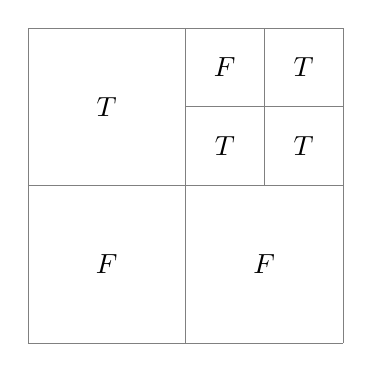
\begin{tikzpicture}
%[my/.style={draw, circle, fill=gray!20!, minimum size=5mm}]
\draw[help lines,step=2cm] (0,0) grid (4,4);
\draw[help lines] (2,2) grid (4,4);
\node at (1,1) {$F$};
\node at (3,1) {$F$};
\node at (1,3) {$T$};
\node at (2.5,2.5) {$T$};
\node at (3.5,2.5) {$T$};
\node at (2.5,3.5) {$F$};
\node at (3.5,3.5) {$T$};
\end{tikzpicture}
\end{figure}

Your task is to implement a function that will take two quadtrees and return a quadtree that represents the logical OR (or union) of the two trees.

\begin{figure}[H]
\begin{minipage}{0.3\linewidth}
\centering
\begin{tikzpicture}
%[my/.style={draw, circle, fill=gray!20!, minimum size=5mm}]
\draw[help lines,step=2cm] (0,0) grid (4,4);
\node at (1,1) {$F$};
\node at (3,1) {$F$};
\node at (1,3) {$T$};
\node at (3,3) {$T$};
\end{tikzpicture}
\end{minipage}
\hfill
\begin{minipage}{0.3\linewidth}
\centering
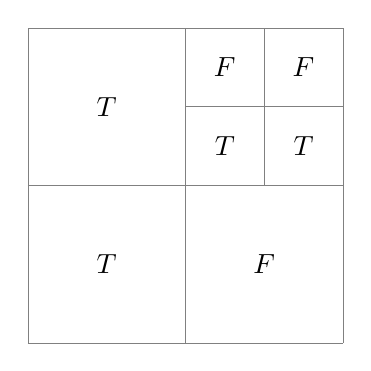
\begin{tikzpicture}
%[my/.style={draw, circle, fill=gray!20!, minimum size=5mm}]
\draw[help lines,step=2cm] (0,0) grid (4,4);
\draw[help lines] (2,2) grid (4,4);
\node at (1,1) {$T$};
\node at (3,1) {$F$};
\node at (1,3) {$T$};
\node at (2.5,2.5) {$T$};
\node at (3.5,2.5) {$T$};
\node at (2.5,3.5) {$F$};
\node at (3.5,3.5) {$F$};
\end{tikzpicture}
\end{minipage}
\hfill
\begin{minipage}{0.3\linewidth}
\centering
\begin{tikzpicture}
\draw[help lines,step=2cm] (0,0) grid (4,4);
\node at (1,1) {$T$};
\node at (3,1) {$F$};
\node at (1,3) {$T$};
\node at (3,3) {$T$};
\end{tikzpicture}
\end{minipage}
\end{figure}

\paragraph{Note:}

\begin{itemize}
\item Both $A$ and $B$ represent grids of size $N \times N$.
\item $N$ is guaranteed to be a power of 2.
\item The logic \textbf{OR} operation is defined as this: $A$ \texttt{or} $B$ is \texttt{true} if $A$ is \texttt{true}, or if $B$ is \texttt{true}, or if both $A$ and $B$ are \texttt{true}.
\end{itemize}

\subsection{Depth First Search}
\begin{itemize}
\item If the one of $A$ and $B$ is leaf and the value is \texttt{True}, the result node is this node. If one of $A$ and $B$ is leaf and the value is \texttt{False}, the result is another node.
\item If both $A$ and $B$ are not leaves, we recursively to get four nodes to represent the intersections of their four child nodes. If these four nodes are all leaves and have same value, we just create and return a new leaf node to store the value.
\item Otherwise, we create and return a non leaf node to store these four nodes.
\end{itemize}

\setcounter{lstlisting}{0}
\begin{lstlisting}[style=customc, caption={DFS}]
Node* intersect( Node* quadTree1, Node* quadTree2 )
{
    if( quadTree1->isLeaf )
    {
        return quadTree1->val ? quadTree1 : quadTree2;
    }

    if( quadTree2->isLeaf )
    {
        return quadTree2->val ? quadTree2 : quadTree1;
    }

    auto tl = intersect( quadTree1->topLeft, quadTree2->topLeft );
    auto tr = intersect( quadTree1->topRight, quadTree2->topRight );
    auto bl = intersect( quadTree1->bottomLeft, quadTree2->bottomLeft );
    auto br = intersect( quadTree1->bottomRight, quadTree2->bottomRight );

    bool one_node = ( tl->isLeaf && tr->isLeaf && bl->isLeaf && br->isLeaf );

    if( one_node )
    {
        if( ( tl->val == tr->val ) && ( bl->val == br->val ) && ( tl->val == bl->val ) )
        {
            one_node = true;
        }
        else
        {
            one_node = false;
        }
    }

    if( one_node )
    {
        auto val = tl->val;
        delete tl;
        delete tr;
        delete bl;
        delete br;
        //create a leaf node represents the four nodes
        return new Node{val, true, nullptr, nullptr, nullptr, nullptr};
    }

    //create a non-leaf node to contains the four nodes
    return new Node{false, false, tl, tr, bl, br};
}
\end{lstlisting}

%\section{559 --- Maximum Depth of N-ary Tree}
Given a $n$-ary tree, find its maximum depth.

The maximum depth is the number of nodes along the longest path from the root node down to the farthest leaf node.

For example, given a \texttt{3-ary} tree:

 
\begin{figure}[H]
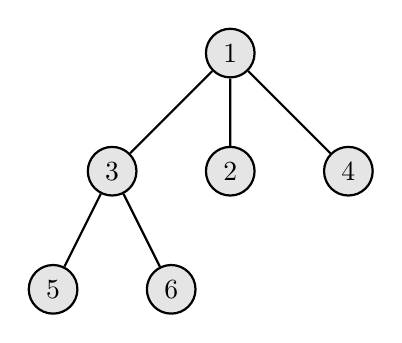
\begin{tikzpicture}
[every node/.style={draw, circle, minimum size=6mm, fill=gray!20!},
  node distance=8mm, 
 thick
]
\node{1}
child{node{3} child{node{5}} child{node{6}}}
child{node{2}}
child{node{4}};
\end{tikzpicture}
\end{figure}

 

We should return its max depth, which is 3.

 

\paragraph{Note:}

\begin{itemize}
\item The depth of the tree is at most 1000.
\item The total number of nodes is at most 5000.
\end{itemize}

\subsection{Recursion}
\begin{itemize}
\item 和计算binary tree的max depth方法类似,对每个child node递归处理,然后结果加上1即为沿着该child node一直往下走的深度。然后所有child node的深度中取最大的深度作为当前node的最大深度。
\end{itemize}

\setcounter{lstlisting}{0}
\begin{lstlisting}[style=customc, caption={Recursion}]
int maxDepth( Node* root )
{
    if( !root )
    {
        return 0;
    }

    int d = 1;

    for( auto node : root->children )
    {
        //1+maxDepth(node) is the depth
        //along with this node
        d = ( max )( d, 1 + maxDepth( node ) );
    }

    return d;
}
\end{lstlisting}
%\section{560 --- Subarray Sum Equals K}
Given an array of integers, $A$, and an integer $ k $, you need to find the total number of continuous subarrays whose sum equals to $ k $.

\paragraph{Example 1:}
\begin{flushleft}
\textbf{Input}: $A = [1,1,1]$, $k = 2$

\textbf{Output}: 2
\end{flushleft}

\paragraph{Note:}
\begin{itemize}
\item The length of the array is in range $[1, 20,000]$.

\item The range of numbers in the array is $[-1000, 1000]$ and the range of the integer $k$ is $[-10^7, 10^7]$.
\end{itemize}

\subsection{Prefix Sum}
\begin{itemize}
\item 记录每个index处的prefix sum $x$,然后看之前的prefix sum是否出现过$x-k$,如果有,将$x-k$出现的次数加入到结果中。
\item 如果$x=k$,将结果加1。
\item 需要一个hash map记录prefix sum及其出现次数。
\end{itemize}

\setcounter{lstlisting}{0}
\begin{lstlisting}[style=customc, caption={Prefix Sum}]
int subarraySum( vector<int>& nums, int k )
{
    unordered_map<int, int> m;

    vector<int> ps( nums.size() + 1, 0 );

    //helper lambda
    //to add to hash map
    auto add_m = [&m]( int n )
    {
        auto it = m.find( n );
        if( it == m.end() )
        {
            m.emplace( n, 1 );
        }
        else
        {
            ++it->second;
        }
    };

    int ans = 0;

    for( size_t i = 0; i < nums.size(); ++i )
    {
        ps[i + 1] = nums[i] + ps[i];


        if( ps[i + 1] == k )
        {
            ++ans;
        }

        int x = ps[i + 1] - k;

        auto it = m.find( x );
        if( it != m.end() )
        {
            //add the count
            ans += it->second;
        }

        //after finding,
        //add the sum to the hash map
        add_m( ps[i + 1] );
    }

    return ans;
}
\end{lstlisting}
%\section{561 --- Array Partition I}
Given an array of $2n$ integers, $A$, your task is to group these integers into $n$ pairs of integer, say $(a_1, b_1)$, $(a_2, b_2)$, $\ldots$, $(a_n, b_n)$ which makes sum of $\min(a_i, b_i)$ for all $i$ from 1 to $n$ as large as possible.

\paragraph{Example 1:}

\begin{flushleft}
\textbf{Input}: $ [1,4,3,2] $

\textbf{Output}: 4

\textbf{Explanation}: $n$ is 2, and the maximum sum of pairs is $4 = \min(1, 2) + \min(3, 4)$.

\end{flushleft}

\paragraph{Note:}
\begin{itemize}
\item $ n $ is a positive integer, which is in the range of $ [1, 10000] $.
\item All the integers in the array will be in the range of $ [-10000, 10000] $.
\end{itemize}

\subsection{Sorting}
\begin{itemize}
\item The total sum will now be maximum if the overall loss incurred from such pairings is minimized. This minimization of loss in every pairing is possible only if the numbers chosen for the pairings lie closer to each other than to the other elements of the array.
\item Taking this into consideration, we can sort the elements of the given array and form the pairings of the elements directly in the sorted order. This will lead to the pairings of elements with minimum difference between them leading to the maximization of the required sum.
\end{itemize}

\setcounter{lstlisting}{0}
\begin{lstlisting}[style=customc, caption={Sorting}]
int arrayPairSum( vector<int>& nums )
{
    sort( nums.begin(), nums.end() );

    int ans = 0;

    for( size_t i = 0; i < nums.size(); i += 2 )
    {
        ans += nums[i];
    }

    return ans;
}
\end{lstlisting}

\subsection{Hash Map}
\begin{itemize}
\item 记录每个数字出现的次数,这里不能用普通的hash map,由于题目给定的数字范围是$ [-10000, 10000] $,可以用一个数组$H$来代替。
\item 如果当前数字$x$出现偶数次,将这些同样的数字进行配对,那么每个pair的最小数字就是$x$。
\item 如果这个数字出现奇数次,那么将$x$与$x+1$进行配对,保证数字之差仍然最小。同时$x+1$的个数会减少一次。
\end{itemize}

\begin{lstlisting}[style=customc, caption={Hash Map}]
int arrayPairSum( vector<int>& nums )
{
    //since all elements are between [-10000, 10000]
    //we can use an array as the hash map
    vector<int> H( 20001, 0 );

    for( int n : nums )
    {
        H[n + 10000] += 1;
    }

    int left = 0;
    int ans = 0;

    for( int x = -10000; x <= 10000; ++x )
    {
        int count = H[x + 10000];

        if( left == 1 )
        {
            //we have to make a pair
            //with x and x-1
            //the minimum for this pair
            //is x-1
            ans += ( x - 1 );
        }

        //remove the one
        //that make pair with last number
        count -= left;

        if( count & 1 )
        {
            //we will have one x left
            //to be paired with x+1
            left = 1;
            --count;
        }
        else
        {
            left = 0;
        }

        //for count/2 pairs of (x,x)
        //the minimum is x
        ans += ( x ) * ( count / 2 );
    }

    return ans;
}
\end{lstlisting}
%\section{562 --- Longest Line of Consecutive One in Matrix}
Given a 01 matrix $M$, find the longest line of consecutive one in the matrix. The line could be horizontal, vertical, diagonal or anti-diagonal.
\paragraph{Example:}

\begin{flushleft}
\textbf{Input}:
[[0,1,1,0],
 [0,1,1,0],
 [0,0,0,1]]
\textbf{Output}: 3

\end{flushleft}

\paragraph{Hint:} 
\begin{itemize}
\item The number of elements in the given matrix will not exceed 10,000.
\end{itemize}

\subsection{Dynamic Programming}
\begin{itemize}
\item 用$F(i,j,k)$代表the length of consecutive ones at $M[i][j]$,其中
\begin{itemize}
\item $k=0$ 表示horizontal
\item $k=1$ 表示vertical
\item $k=2$ 表示diagonal
\item $k=3$ 表示anti-diagonal
\end{itemize}
\item 如果$M[i][j]=1$,分别 check $M[i-1][j]$, $M[i][j-1]$, $M[i-1][j-1]$ 和 $M[i-1][j+1]$是否为1。 如果是1,那么$F(i,j,k)\gets F(i,j,k)+1$,否则$F(i,j,k)=1$。
\item 如果$M[i][j]=0$, 那么$F(i,j,k)=0$
\item Maintain一个变量,记录遇到的最大长度。
\end{itemize}

\setcounter{lstlisting}{0}
\begin{lstlisting}[style=customc, caption={Dynamic Programming}]
int longestLine( vector<vector<int>>& M )
{

    if( M.empty() || M[0].empty() )
    {
        return 0;
    }

    using count_t = array<int, 4>;

    vector<vector<count_t>> F( M.size(), vector<count_t>( M[0].size(), count_t{0, 0, 0, 0} ) );


    int ans = 0;

    for( size_t r = 0; r < M.size(); ++r )
    {
        for( size_t c = 0; c < M[0].size(); ++c )
        {
            if( M[r][c] == 1 )
            {
                //the length of each direction
                //is at least 1
                F[r][c][0] = 1;
                F[r][c][1] = 1;
                F[r][c][2] = 1;
                F[r][c][3] = 1;

                if( ( r > 0 ) || ( c > 0 ) )
                {
                    if( ( r > 0 ) && ( M[r - 1][c] == 1 ) )
                    {
                        //the horizon length increments
                        F[r][c][0] = F[r - 1][c][0] + 1;
                    }

                    if( ( c > 0 ) && ( M[r][c - 1] == 1 ) )
                    {
                        //the vertical length increments
                        F[r][c][1] = F[r][c - 1][1] + 1;
                    }

                    if( ( r > 0 ) && ( c > 0 ) && ( M[r - 1][c - 1] == 1 ) )
                    {
                        //the diag length increments
                        F[r][c][2] = F[r - 1][c - 1][2] + 1;
                    }

                    if( ( r > 0 ) && ( c < M[0].size() - 1 ) && ( M[r - 1][c + 1] == 1 ) )
                    {
                        //the anti-diag length increments
                        F[r][c][3] = F[r - 1][c + 1][3] + 1;
                    }
                }

                //get the maximum length so far
                ans = ( max )( ans, F[r][c][0] );
                ans = ( max )( ans, F[r][c][1] );
                ans = ( max )( ans, F[r][c][2] );
                ans = ( max )( ans, F[r][c][3] );
            }//outmost if
        } //inner for
    }//outer for

    return ans;
}
\end{lstlisting}
%\section{563 --- Binary Tree Tilt}
Given a binary tree, return the tilt of the \textbf{whole tree}.

The tilt of a \textbf{tree node} is defined as the \textbf{absolute difference} between the sum of all left subtree node values and the sum of all right subtree node values. Null node has tilt 0.

The tilt of the \textbf{whole tree} is defined as the sum of all nodes' tilt.

\paragraph{Example:}
\begin{flushleft}
\textbf{Input}: 
\begin{figure}[H]
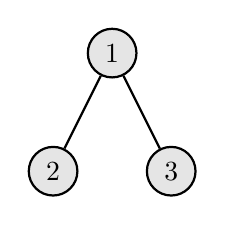
\begin{tikzpicture}
[every node/.style={draw, circle,minimum size=6mm, fill=gray!20!},
  node distance=8mm, thick]
\node{1}
child{node{2}}
child{node{3}};
\end{tikzpicture}
\end{figure}

\textbf{Output}: 1

\textbf{Explanation}: 

Tilt of node 2 : 0

Tilt of node 3 : 0

Tilt of node 1 : $\lvert 2-3\rvert = 1$

Tilt of binary tree : $0 + 0 + 1 = 1$
\end{flushleft}

\paragraph{Note:}

\begin{itemize}
\item The sum of node values in any subtree won't exceed the range of 32-bit integer.
\item All the tilt values won't exceed the range of 32-bit integer.
\end{itemize}

\subsection{Recursion}
\begin{itemize}
\item 递归函数应返回以某个node为根节点的tree的所有node的sum。
\item 分别对node的左右节点进行递归,将左右两个子树的sum的差的绝对值加入到最终结果中。
\end{itemize}

\setcounter{lstlisting}{0}
\begin{lstlisting}[style=customc, caption={Recursion}]
int findTilt( TreeNode* root )
{

    int ans = 0;

    dfs( root, ans );

    return ans;
}

//get the sum of all nodes in the tree
//rooted at node
//tilt is the by product of this function
int dfs( TreeNode* node, int& tilt )
{
    if( !node )
    {
        return 0;
    }

    //get left subtree sum
    int left = dfs( node->left, tilt );
    //get right subtree sum
    int right = dfs( node->right, tilt );

    tilt += abs( left - right );

    return node->val + left + right;
}
\end{lstlisting}
%\section{564 --- Find the Closest Palindrome}
Given an integer $n$, find the closest integer (not including itself), which is a palindrome.

The \textbf{closest} is defined as absolute difference minimized between two integers.

\paragraph{Example 1:}
\begin{flushleft}
\textbf{Input}: $ 123 $

\textbf{Output}: $ 121 $
\end{flushleft}

\paragraph{Note:}
\begin{itemize}
\item The input $ n $ is a positive integer represented by string, whose length will not exceed 18.
\item If there is a tie, return the smaller one as answer.
\end{itemize}

\subsection{Mathematical Approach}
首先可以得到结论, 如果需要通过copy一半字符的方式从$n$得到 Palindrome number,那么一定是copy first half 到 second half.

其次,有三种方式对$n$进行转换得到距离最近的Palindrome number
\begin{enumerate}
\item Copy first half to second half. For example:  Suppose $n=10987$. After this kind of transformation, we can get $10901$.
\item Decrement the first half and then copy first half.
\item Increment the first half and then copy first half.
\item If the digit at the middle index is zero, decrement the first half and then copy first half: For example, when $n=20001$, decrements the first half $200$ we get $199$, then copy to second half we get $19991$. .
\item If the digit at the middle index is $9$, increments the second half and then copy first half: For example, when $n=10987$, increments the first half $109$ we get $110$, then copy to second half we get $11011$. We do not decrement first half in this case because the generated number must have larger difference than just copying the first half to second half.
\end{enumerate}

\section{565 --- Array Nesting}

\textbf{Medium}

A zero-indexed array $A$ of length $N$ contains all integers from 0 to $N-1$. Find and return the longest length of set $S$, where $S[i] = {A[i], A[A[i]], A[A[A[i]]], \ldots }$ subjected to the rule below.

Suppose the first element in $S$ starts with the selection of element $A[i]$ of index $i$, the next element in $S$ should be $A[A[i]]$, and then $A[A[A[i]]]$, $\ldots$. By that analogy, we stop adding right before a duplicate element occurs in $S$.

 

\paragraph{Example 1:}

\begin{flushleft}
\textbf{Input}: \fcj{A = [5,4,0,3,1,6,2]}

\textbf{Output}: 4

\textbf{Explanation}: 

A[0] = 5, A[1] = 4, A[2] = 0, A[3] = 3, A[4] = 1, A[5] = 6, A[6] = 2.

One of the longest \fcj{S[K]}:

\fcj{S[0] = {A[0], A[5], A[6], A[2]} = {5, 6, 2, 0}}
\end{flushleft}
 

\paragraph{Note:}

\begin{itemize}
\item $N$ is an integer within the range \fcj{[1, 20,000]}.

\item The elements of A are all distinct.

\item Each element of A is an integer within the range \fcj{[0, N-1]}.
\end{itemize}

\subsection{Using Visited Array}
We will notice a fact that we will always reach a point where the current element becomes equal to the element \fcj{nums[i]} with which we started the nestings in the first place. 

Thus, after this, the new indices generated will be just the repetitions of the previously generated ones, and thus would not lead to an increase in the size of the current set.

Thus, this condition of the current number being equal to the starting number acts as the terminating condition for a particular index.

Instead of making use of a separate array to keep track of the same, we can mark the visited elements in the original array as a special value.

\setcounter{lstlisting}{0}
\begin{lstlisting}[style=customc, caption={Visited Array}]
int arrayNesting( vector<int>& nums )
{
    int N = ( int )( nums.size() );
    int ans = 1;
    for( size_t i = 0; i < nums.size(); ++i )
    {
        if( nums[i] != N + 100 )
        {
            //nums[i] is not visisted
            int start = nums[i];
            int count = 0;
            while( nums[start] != N + 100 )
            {
                //proceed in the loop
                int tmp = start;
                start = nums[start];
                ++count;
                //mark nums[tmp] as visited
                nums[tmp] = N + 100;
            }
            //update maximum count so far
            ans = ( max )( ans, count );
        }
    }
    return ans;
}
\end{lstlisting}

\paragraph{Related Problems}
\begin{itemize}
\item \textbf{339. Nested List Weight Sum}
\item \textbf{341. Flatten Nested List Iterator}
\item \textbf{364. Nested List Weight Sum II}
\end{itemize}
%\include{566}
%\include{567}
%\include{568}
%\include{569}
%\include{570}
%\include{571}
%\section{572 --- Subtree of Another Tree}
Given two non-empty binary trees $s$ and $t$, check whether tree $ t $ has exactly the same structure and node values with a subtree of $ s $. A subtree of $ s $ is a tree consists of a node in $ s $ and all of this node's descendants. The tree $ s $ could also be considered as a subtree of itself.

\paragraph{Example 1:}
\begin{flushleft}
\textbf{Input}:
Given tree $s$:
\begin{figure}[H]
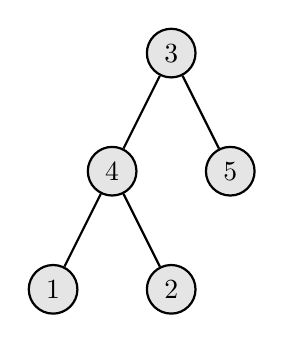
\begin{tikzpicture}
[every node/.style={draw, circle,minimum size=6mm, fill=gray!20!},
  node distance=8mm, thick]
\node{3}
child{node{4} child{node{1}} child{node{2}}}
child{node{5}};
\end{tikzpicture}
\end{figure}

Given tree $t$:

\begin{figure}[H]
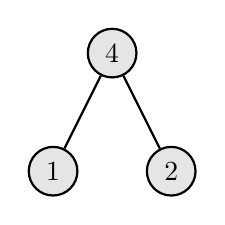
\begin{tikzpicture}
[every node/.style={draw, circle,minimum size=6mm, fill=gray!20!},
  node distance=8mm, thick]
\node{4} 
child{node{1}}
child{node{2}};
\end{tikzpicture}
\end{figure}

\textbf{Output}: \texttt{true}

\textbf{Explanation}: because $t$ has the same structure and node values with a subtree of $s$.
\end{flushleft}

\paragraph{Example 2:}

\begin{flushleft}
Given tree $s$:
\begin{figure}[H]
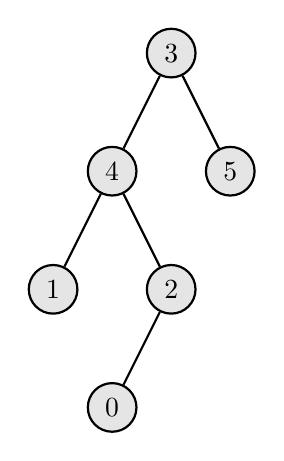
\begin{tikzpicture}
[every node/.style={draw, circle,minimum size=6mm, fill=gray!20!},
  node distance=8mm, thick]
\node{3}
child{node{4} child{node{1}} child{node{2} child{node{0}} child[missing]}}
child{node{5}};
\end{tikzpicture}
\end{figure}

Given tree $t$:
\begin{figure}[H]
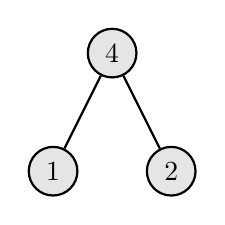
\begin{tikzpicture}
[every node/.style={draw, circle,minimum size=6mm, fill=gray!20!},
  node distance=8mm, thick]
\node{4} 
child{node{1}}
child{node{2}};
\end{tikzpicture}
\end{figure}

\textbf{Output}: \texttt{false}
\end{flushleft}

\subsection{Recursion}
\begin{itemize}
\item We need a helper function to check if two binary tree are equal, i.e., they have same structure and values.
\item In the main function, first we check if the binary tree rooted with $s$ is equal to $t$ or not. If they are equal, just return \texttt{true}. Otherwise, we recursively call the main function to compare left/right child tree of $s$ against $t$. If either case return \texttt{true}, we just return \texttt{true}.
\item We do not call the helper function to recursively compare left/right child tree of $s$ against $t$. The reason is that helper function only check two trees with fixed root. For example, if left child tree of $s$ is not equal to $t$, the helper function will not recursively to try the left grandchild or right grandchild of $s$.
\end{itemize}

\setcounter{lstlisting}{0}
\begin{lstlisting}[style=customc, caption={Recursion}]
bool isSubtree( TreeNode* s, TreeNode* t )
{
    if( equal( s, t ) )
    {
        return true;
    }

    if( s )
    {
        //compare left/right child of s to t
        return isSubtree( s->left, t ) || isSubtree( s->right, t );
    }

    return false;
}

//helper function to check if s and t
//has same structure and node values.
//s and t are fixed.
bool equal( TreeNode* s, TreeNode* t )
{
    if( !s && !t )
    {
        return true;
    }

    if( !s || !t )
    {
        return false;
    }

    if( s->val == t->val )
    {
        return equal( s->left, t->left ) && equal( s->right, t->right );
    }

    return false;
}
\end{lstlisting}
%\section{573 --- Squirrel Simulation}
There's a tree, a squirrel, and several nuts. Positions are represented by the cells in a 2D grid. Your goal is to find the \textbf{minimal} distance for the squirrel to collect all the nuts and put them under the tree one by one. The squirrel can only take at most \textbf{one nut} at one time and can move in four directions -- up, down, left and right, to the adjacent cell. The distance is represented by the number of moves.

\paragraph{Example 1:}

\begin{flushleft}
\textbf{Input}: 

$H:=5$, $W:=7$, 

Tree position : $[2,2]$

Squirrel : $[4,4]$

Nuts : $[[3,0], [2,5]]$

\textbf{Output}: 12

\textbf{Explanation}:
\begin{figure}[H]
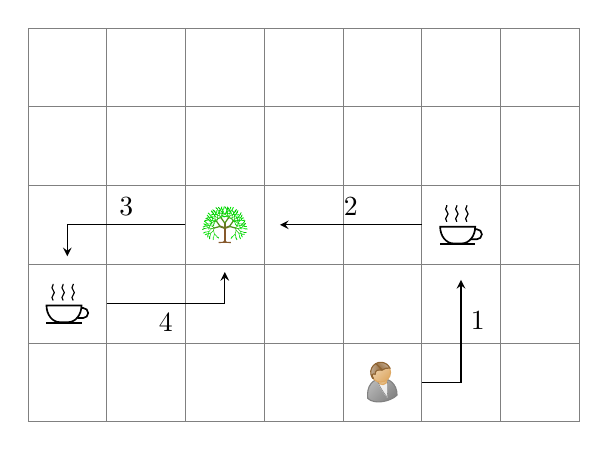
\begin{tikzpicture}
\draw[help lines] (0,0) grid (7, 5);
\node[bob] at (4.5, 0.5) {};
\node at (5.5,2.5) {\Coffeecup[2]};
\node at (0.5,1.5) {\Coffeecup[2]};
\node at (2.5, 2.5) {\Springtree[2]};
\draw[>=stealth, ->] (5,0.5) -| (5.5, 1.8) node[pos=0.80, right] {1};
\draw[>=stealth, ->] (5,2.5) -> (3.2, 2.5) node[midway, above] {2};
\draw[>=stealth, ->] (2,2.5) -| (0.5, 2.1) node[pos=0.25, above] {3};
\draw[>=stealth, ->] (1,1.5) -| (2.5, 1.9) node[pos=0.25, below] {4};
\end{tikzpicture}
\end{figure}

\end{flushleft}

\paragraph{Note:}

\begin{itemize}
\item All given positions won't overlap.
\item The squirrel can take at most one nut at one time.
\item The given positions of nuts have no order.
\item Height, $H$, and Width, $W$, are positive integers. $3 \leq H\times W \leq 10,000$.
\item The given positions contain at least one nut, only one tree and one squirrel.
\end{itemize}


%\include{574}
%\include{575}
%\include{576}
%\include{577}
%\include{578}
%\include{579}
%\include{580}
%\include{581}
%\include{582}
%\include{583}
%\include{584}
%\include{585}
%\include{586}
\section{587 --- Erect the Fence}
There are some trees, where each tree is represented by $(x,y)$ coordinate in a two-dimensional garden. Your job is to fence the entire garden using the minimum length of rope as it is expensive. The garden is well fenced only if all the trees are enclosed. Your task is to help find the coordinates of trees which are exactly located on the fence perimeter.

\paragraph{Example 1:}

\begin{flushleft}
\textbf{Input}: $[[1,1],[2,2],[2,0],[2,4],[3,3],[4,2]]$

\textbf{Output}: $[[1,1],[2,0],[4,2],[3,3],[2,4]]$

\textbf{Explanation}
\begin{figure}[H]
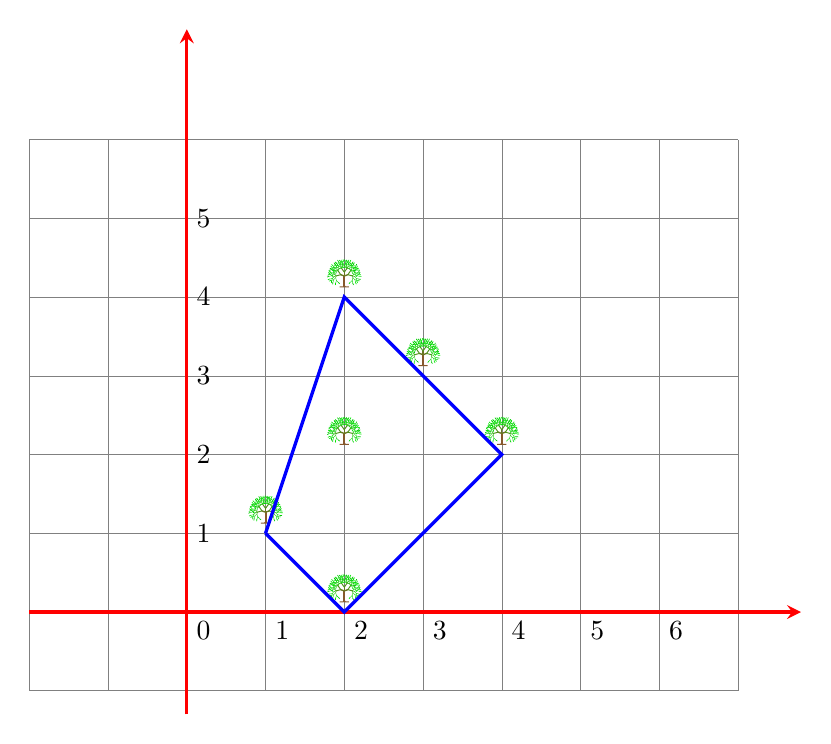
\begin{tikzpicture}
\draw[help lines] (0,0) grid (9,7);
\node at (3,2) [anchor=south] {\Springtree[1.5]};
\node at (4,3) [anchor=south]{\Springtree[1.5]};
\node at (4,1) [anchor=south]{\Springtree[1.5]};
\node at (4,5) [anchor=south]{\Springtree[1.5]};
\node at (5,4) [anchor=south]{\Springtree[1.5]};
\node at (6,3) [anchor=south]{\Springtree[1.5]};
\draw[very thick, >=stealth, ->, red] (0,1) -- (9.8,1);
\draw[very thick, >=stealth, ->, red] (2,-0.3) -- (2,8.4);
\draw[very thick, blue] (3,2) -- (4,1) -- (6,3) -- (5,4) -- (4,5) -- (3,2);
\foreach \x/\y in {2/0,3/1,4/2,5/3,6/4,7/5,8/6}
{\node at (\x, 1) [anchor=north west] {\y};
}
\foreach \x/\y in {2/1,3/2,4/3,5/4,6/5}
{
\node at (2,\x) [anchor=west] {\y};
}

\end{tikzpicture}
\end{figure}
\end{flushleft}

\paragraph{Example 2:}

\begin{flushleft}

\textbf{Input}: $[[1,2],[2,2],[4,2]]$

\textbf{Output}: $[[1,2],[2,2],[4,2]]$

\textbf{Explanation}:

Even you only have trees in a line, you need to use rope to enclose them. 

\begin{figure}[H]
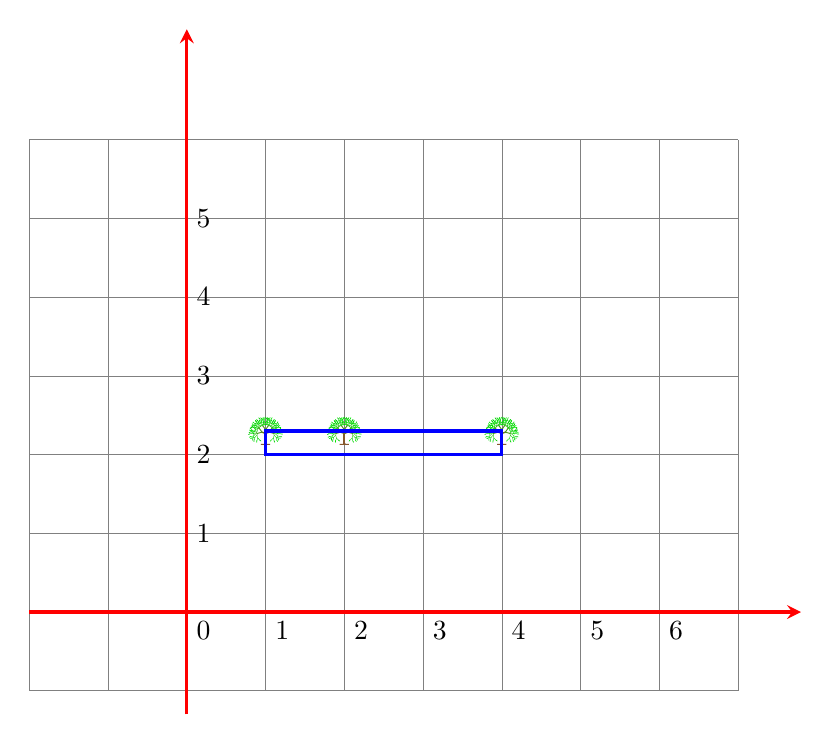
\begin{tikzpicture}
\draw[help lines] (0,0) grid (9,7);
\node at (3,3) [anchor=south] {\Springtree[1.5]};
\node at (4,3) [anchor=south]{\Springtree[1.5]};
\node at (6,3) [anchor=south]{\Springtree[1.5]};
\draw[very thick, >=stealth, ->, red] (0,1) -- (9.8,1);
\draw[very thick, >=stealth, ->, red] (2,-0.3) -- (2,8.4);
\draw[very thick, blue] (3,3) rectangle ++(3, 0.3);
\foreach \x/\y in {2/0,3/1,4/2,5/3,6/4,7/5,8/6}
{\node at (\x, 1) [anchor=north west] {\y};
}
\foreach \x/\y in {2/1,3/2,4/3,5/4,6/5}
{
\node at (2,\x) [anchor=west] {\y};
}

\end{tikzpicture}
\end{figure} 

\end{flushleft}

\paragraph{Note:}

\begin{itemize}
\item All trees should be enclosed together. You cannot cut the rope to enclose trees that will separate them in more than one group.
\item All input integers will range from 0 to 100.
\item The garden has at least one tree.
\item All coordinates are distinct.
\item Input points have NO order. No order required for output.
\end{itemize}

\subsection{Find Convex Hull}
\section{588 --- Design In-Memory File System}
Design an in-memory file system to simulate the following functions:

\begin{itemize}
\item \texttt{ls}: Given a path in string format. If it is a file path, return a list that only contains this file's name. If it is a directory path, return the list of file and directory names in \textbf{this directory}. Your output (file and directory names together) should in \textbf{lexicographic order}.

\item \texttt{mkdir}: Given a \textbf{directory path} that does not exist, you should make a new directory according to the path. If the middle directories in the path don't exist either, you should create them as well. This function has void return type.

\texttt{addContentToFile}: Given a \textbf{file path} and \textbf{file content} in string format. If the file doesn't exist, you need to create that file containing given content. If the file already exists, you need to \textbf{append} given content to original content. This function has void return type.

\texttt{readContentFromFile}: Given a \textbf{file path}, return its \textbf{content} in string format.
\end{itemize}

 
\paragraph{Note:}

\begin{itemize}
\item You can assume all file or directory paths are absolute paths which begin with slash and do not end with slash except that the path is just only slash.
\item You can assume that all operations will be passed valid parameters and users will not attempt to retrieve file content or list a directory or file that does not exist.
\item You can assume that all directory names and file names only contain lower-case letters, and same names won't exist in the same directory.
\end{itemize}

\subsection{Trie}
\begin{itemize}
\item Design this filesystem data structure as a Trie where each node represent a struct, say, \texttt{File}.
\end{itemize}

\setcounter{lstlisting}{0}
\begin{lstlisting}[style=customc, caption={Trie}]
class FileSystem
{
public:
    FileSystem()
    {

        root = make_unique<File>();
    }

    vector<string> ls( string path )
    {

        istringstream iss( path );

        string token;

        auto node = root.get();

        while( getline( iss, token, '/' ) )
        {
            if( token.empty() )
            {
                continue;
            }
            auto it = node->files.find( token );

            if( it == node->files.end() )
            {
                return {};
            }

            node = it->second.get();
        }

        if( node->flag == 1 )
        {
            //this is file
            //only output the file name

            auto pos = path.find_last_of( '/' );
            return {path.substr( pos + 1 )};
        }

        vector<string> ans;

        for( const auto& file : node->files )
        {
            //add files into the list
            ans.push_back( file.first );
        }

        sort( begin( ans ), end( ans ) );

        return ans;
    }

    void mkdir( string path )
    {

        istringstream iss( path );

        string token;

        auto node = root.get();

        while( getline( iss, token, '/' ) )
        {

            if( token.empty() )
            {
                continue;
            }

            auto it = node->files.find( token );


            if( it == node->files.end() )
            {
                //this directory doesn't exist
                //create a new one
                it = node->files.emplace( token, make_unique<File>() ).first;
            }

            node = it->second.get();
        }
    }

    void addContentToFile( string filePath, string content )
    {

        istringstream iss( filePath );

        string token;

        auto node = root.get();

        while( getline( iss, token, '/' ) )
        {
            if( token.empty() )
            {
                continue;
            }

            auto it = node->files.find( token );

            if( it == node->files.end() )
            {
                it = node->files.emplace( token, make_unique<File>() ).first;
            }

            node = it->second.get();
        }

        node->flag = 1; //this is file
        node->content.append( move( content ) );
    }

    string readContentFromFile( string filePath )
    {

        istringstream iss( filePath );

        string token;

        auto node = root.get();

        while( getline( iss, token, '/' ) )
        {
            if( token.empty() )
            {
                continue;
            }
            auto it = node->files.find( token );
            if( it == node->files.end() )
            {
                //The path doesn't exist
                return "";
            }

            node = it->second.get();
        }

        if( node->flag )
        {
            return node->content;
        }

        //this path is not a file
        return "";
    }

private:

    struct File
    {
        unsigned char flag = 0;

        unordered_map<string, unique_ptr<File>> files;

        string content;
    };

    unique_ptr<File> root;
};
\end{lstlisting}
\section{589 --- N-ary Tree Preorder Traversal}
Given an $n$-ary tree, return the \textit{preorder} traversal of its nodes' values.

For example, given a 3-ary tree:

\begin{figure}[H]
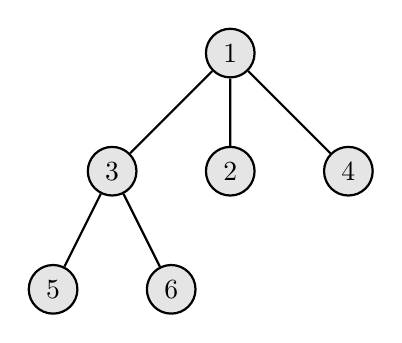
\begin{tikzpicture}
[every node/.style={draw, circle,minimum size=6mm, fill=gray!20!}, node distance=8mm,thick]
\node{1}
child{node{3} child{node{5}} child{node{6}}}
child{node{2}}
child{node{4}};
\end{tikzpicture}
\end{figure}

Return its preorder traversal as: $[1,3,5,6,2,4]$.


\paragraph{Note:}

\begin{itemize}
\item Recursive solution is trivial, could you do it iteratively?
\end{itemize}

\subsection{Stack}
\begin{itemize}
\item Iteration method is similar to binary tree, we insert the children nodes into the stack reversely.
\end{itemize}

\setcounter{lstlisting}{0}
\begin{lstlisting}[style=customc, caption={Stack}]
vector<int> preorder( Node* root )
{
    stack<Node*> stk;
    stk.push( root );

    vector<int> ans;

    while( !stk.empty() )
    {
        auto t = stk.top();
        stk.pop();

        if( !t )
        {
            break;
        }

        ans.push_back( t->val );

        if( t->children.empty() )
        {
            continue;
        }

        for( size_t i = 0; i < t->children.size(); ++i )
        {
            //put the childre per the reverse order
            //into the stack
            auto j = t->children.size() - i - 1;
            stk.push( t->children[j] );
        }

    }
    return ans;
}
\end{lstlisting}
\section{590 --- N-ary Tree Postorder Traversal}
Given an $n$-ary tree, return the \textit{postorder} traversal of its nodes' values.

For example, given a 3-ary tree:

\begin{figure}[H]
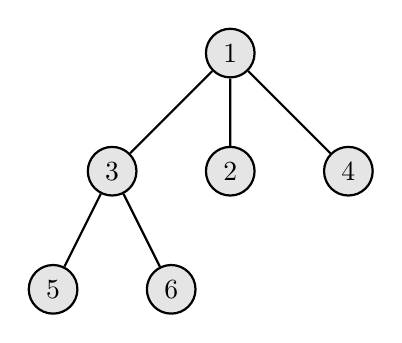
\begin{tikzpicture}
[every node/.style={draw, circle,minimum size=6mm, fill=gray!20!}, node distance=8mm,thick]
\node{1}
child{node{3} child{node{5}} child{node{6}}}
child{node{2}}
child{node{4}};
\end{tikzpicture}
\end{figure}

Return its postorder traversal as: $[5,6,3,2,4,1]$.


\paragraph{Note:}

\begin{itemize}
\item Recursive solution is trivial, could you do it iteratively?
\end{itemize}

\subsection{Stack}
\begin{itemize}
\item Similar to binary tree preorder traverse, we make use of a stack.
\item First, push the root into the stack.
\item At each iteration, pop the top node from the stack, add the value to the output and then push its children from start to end to the stack. 
\item Finally, we need to reverse the output.
\end{itemize}

\setcounter{lstlisting}{0}
\begin{lstlisting}[style=customc, caption={Stack}]
vector<int> postorder( Node* root )
{
    if( !root )
    {
        return {};
    }

    stack<Node*> stk;

    stk.push( root );

    vector<int> ans;

    while( !stk.empty() )
    {
        auto t = stk.top();
        stk.pop();
        ans.push_back( t->val );

        for( auto node : t->children )
        {
            //push the children sequentially
            stk.push( node );
        }
    }

    //we have to reverse the output
    reverse( begin( ans ), end( ans ) );

    return ans;
}
\end{lstlisting}
\section{591 --- Tag Validator}
Given a string, $S$, representing a code snippet, you need to implement a tag validator to parse the code and return whether it is valid. A code snippet is valid if all the following rules hold:

\begin{enumerate}
\item The code must be wrapped in a \textbf{valid closed tag}. Otherwise, the code is invalid.
\item A \textbf{closed tag} (not necessarily valid) has exactly the following format:

 \texttt{<TAG\_NAME>TAG\_CONTENT</TAG\_NAME>}.
 
Among them, \texttt{<TAG\_NAME>} is the start tag, and \texttt{</TAG\_NAME>} is the end tag. The \texttt{TAG\_NAME} in start and end tags should be the same. A closed tag is \textbf{valid} if and only if the \texttt{TAG\_NAME} and \texttt{TAG\_CONTENT} are valid.
\item A \textbf{valid} \texttt{TAG\_NAME} only contain upper-case letters, and has length in range $[1,9]$. Otherwise, the \texttt{TAG\_NAME} is invalid.
\item A \textbf{valid} \texttt{TAG\_CONTENT} may contain other \textbf{valid closed tags}, \textbf{cdata} and any characters EXCEPT unmatched \texttt{<}, unmatched start and end tag, and unmatched or closed tags with invalid \texttt{TAG\_NAME}. Otherwise, the \texttt{TAG\_CONTENT} is invalid.
\item A start tag is unmatched if no end tag exists with the same \texttt{TAG\_NAME}, and vice versa. However, you also need to consider the issue of unbalanced when tags are nested.
\item A \texttt{<} is unmatched if you cannot find a subsequent \texttt{>}. And when you find a \texttt{<} or \texttt{</}, all the subsequent characters until the next \texttt{>} should be parsed as \texttt{TAG\_NAME} (not necessarily valid).
\item The \textbf{cdata} has the following format : \texttt{<![CDATA[CDATA\_CONTENT]]>}. The range of \texttt{CDATA\_CONTENT} is defined as the characters between \texttt{<![CDATA[} and the first subsequent \texttt{]]>}.
\item \texttt{CDATA\_CONTENT} may contain any characters. The function of cdata is to forbid the validator to parse \texttt{CDATA\_CONTENT}, so even it has some characters that can be parsed as tag (no matter valid or invalid), you should treat it as regular characters.
\end{enumerate}

\paragraph{Valid Code Examples:}

\begin{flushleft}
\textbf{Input}: \texttt{<DIV>This is the first line <![CDATA[<div>]]></DIV>}

\textbf{Output}: \texttt{True}

\textbf{Explanation}: 

The code is wrapped in a closed tag : \texttt{<DIV>} and \texttt{</DIV>}. 

The \texttt{TAG\_NAME} is valid, the \texttt{TAG\_CONTENT} consists of some characters and cdata. 

Although \texttt{CDATA\_CONTENT} has unmatched start tag with invalid \texttt{TAG\_NAME}, it should be considered as plain text, not parsed as tag.

So \texttt{TAG\_CONTENT} is valid, and then the code is valid. Thus return \textbf{true}.


\textbf{Input}: \texttt{<DIV>>>  ![cdata[]] <![CDATA[<div>]>]]>]]>>]</DIV>}

\textbf{Output}: \texttt{True}

\textbf{Explanation}:

We first separate the code into : \texttt{start\_tag|tag\_content|end\_tag}.

\texttt{start\_tag}: \texttt{<DIV>}

\texttt{end\_tag}: \texttt{</DIV>}

\texttt{tag\_content} could also be separated into : \texttt{text1|cdata|text2}.

\texttt{text1}: \texttt{>>  ![cdata[]]}

\texttt{cdata}: \texttt{<![CDATA[<div>]>]]>}, where the \texttt{CDATA\_CONTENT} is \texttt{<div>]>}

\texttt{text2}: \texttt{]]>>]}

The reason why \texttt{start\_tag} is NOT \texttt{<DIV>>>} is because of the rule 6.

The reason why \texttt{cdata} is NOT \texttt{<![CDATA[<div>]>]]>]]>} is because of the rule 7.
\end{flushleft}

%Invalid Code Examples:
%Input: "<A>  <B> </A>   </B>"
%Output: False
%Explanation: Unbalanced. If "<A>" is closed, then "<B>" must be unmatched, and vice versa.
%
%Input: "<DIV>  div tag is not closed  <DIV>"
%Output: False
%
%Input: "<DIV>  unmatched <  </DIV>"
%Output: False
%
%Input: "<DIV> closed tags with invalid tag name  <b>123</b> </DIV>"
%Output: False
%
%Input: "<DIV> unmatched tags with invalid tag name  </1234567890> and <CDATA[[]]>  </DIV>"
%Output: False
%
%Input: "<DIV>  unmatched start tag <B>  and unmatched end tag </C>  </DIV>"
%Output: False
%Note:
%For simplicity, you could assume the input code (including the any characters mentioned above) only contain letters, digits, '<','>','/','!','[',']' and ' '.

\subsection{Stack}

Summarizing the given problem, we need to determine whether a tag is valid or not, by checking the following properties.

\begin{itemize}
\item The code should be wrapped in valid closed tag.

\item The \color{red}{\texttt{TAG\_NAME}} should be valid.

\item The \texttt{TAG\_CONTENT} should be valid.

\item The \texttt{cdata} should be valid.
\end{itemize}

All the tags should be closed. i.e. each start-tag should have a corresponding end-tag and vice-versa and the order of the tags should be correct as well.

In order to check the validity of all these, firstly, we need to identify which parts of $S$ act as which part from the above mentioned categories.

\begin{itemize}
\item Iterate over $S$. Whenever a \texttt{<} is encountered( unless we are currently inside \textbf{cdata} section ), it indicates the beginning of either a \texttt{TAG\_NAME}(start tag or end tag) or the beginning of cdata as per the conditions given in the problem statement.

\item If the character immediately following this \texttt{<} is an \texttt{!}, the characters following this \texttt{\textless} can't be a part of a valid \texttt{TAG\_NAME}, since only upper-case letters(in case of a start tag) or \texttt{\textbackslash} followed by upper-case letters(in the case of an end tag). Thus, the choice now narrows down to only \textbf{cdata}. Thus, we need to check if the current bunch of characters following \texttt{\textless!}(including it) constitute a valid cdata. For doing this, firstly we find out the first matching \texttt{]]\textgreater} following the current \texttt{\textless\textexclamdown} to mark the ending of cdata. If no such matching \texttt{]]\textgreater} exists, $S$ is considered as invalid. Apart from this, the \texttt{\textless!} should also be immediately followed by \texttt{CDATA[} for the cdata to be valid. The characters lying inside the \texttt{\textless!CDATA[} and \texttt{]]\textgreater} do not have any constraints on them.

\item If the character immediately following the \texttt{<} encountered isn't an \texttt{!}, this \texttt{<} can only mark the beginnning of \texttt{TAG\_NAME}. Now, since a valid start tag can't contain anything except upper-case letters, if a \texttt{\textbackslash} is found after \texttt{<}, the \texttt{</} pair indicates the beginning of an end tag. Now, when a \texttt{<} refers to the beginning of a \texttt{TAG\_NAME}(either start-tag or end-tag), we find out the first closing \texttt{>} following the \texttt{<} to find out the substring(say $t$), that constitutes the \texttt{TAG\_NAME}. $t$ should satisfy all the criterion to constitute a valid \texttt{TAG\_NAME}. Thus, for every such $t$, we check if it contains all upper-case letters and also check its length(It should be between 1 to 9). If any of the criteria isn't fulfilled, $t$ is not a valid \texttt{TAG\_NAME}. Hence, $S$ is invalid as well.
\
\item Apart from checking the validity of the \texttt{TAG\_NAME}, we also need to ensure that the tags always exist in pairs. i.e. for every start-tag, a corresponding end-tag should always exist. Further, we can note that in case of multiple \texttt{TAG\_NAME}s, the \texttt{TAG\_NAME} whose start-tag comes later than the other ones, should have its end-tag appearing before the end-tags of those other \texttt{TAG\_NAME}s. i.e. the tag which starts later should end first.

\item From this, we get the intuition that we can make use of a stack, $Z$,to check the existence of matching start and end-tags. Thus, whenever we find out a valid start-tag, as mentioned above, we push its \texttt{TAG\_NAME} onto $Z$. Now, whenever an end-tag is found, we compare its \texttt{TAG\_NAME} with the \texttt{TAG\_NAME} at the top of $Z$ and remove this element from $Z$. If the two don't equal, $S$ is invalid.

\item After completing scanning of $S$, the stack $Z$ should be empty if all the start-tags have matched their corresponding end-tags. If $Z$ isn't empty, this implies that some start-tags doesn't have the corresponding end-tags.

\item Further, we also need to ensure that $S$ is completely enclosed within closed tags. Thus, we need to ensure that the first \textbf{cdata} found is also inside the closed tags. Thus, when we find a possibility of the presence of \texttt{cdata}, we proceed further only if we've already found a start tag, indicated by a non-empty stack, $Z$. Further, to ensure that no data lies after the last end-tag, we need to ensure that $Z$ doesn't become empty before we reach the end of $S$, since an empty stack indicates that the last end-tag has been encountered.
\end{itemize}

\setcounter{lstlisting}{0}
\begin{lstlisting}[style=customc, caption={Stack}]
bool isValid( string code )
{
    stack<string> stk;

    bool flag_start_tag = false;

    if( ( code[0] != '<' ) || ( code.back() != '>' ) )
    {
        return false;
    }

    auto is_cdata = []( const string & s, size_t start, size_t end )
    {
        auto pos = s.find( "[CDATA[", start );
        return pos != string::npos;
        //return s.compare( start, end - start, "[CDATA[" ) == 0;
    };


    auto is_valid_tagname = [&stk, &flag_start_tag]( const string & s, size_t start, size_t end, bool end_flag )
    {
        if( ( end == start ) || ( end - start > 9 ) )
        {
            //the tag name must not empty
            //and cannot be larger than 9 letters
            return false;
        }

        for( size_t i = start; i < end; ++i )
        {
            //only uppercase for tagname
            if( ( s[i] >= 'A' ) && ( s[i] <= 'Z' ) )
            {
                continue;
            }

            return false;
        }

        if( end_flag )
        {
            if( !stk.empty() )
            {
                const auto& tagname = stk.top();

                if( s.compare( start, end - start, tagname ) == 0 )
                {
                    stk.pop();
                    return true;
                }
            }

            return false;
        }
        else
        {
            //this is starting tag
            flag_start_tag = true;
            stk.emplace( s, start, end - start );
        }

        return true;
    };

    for( size_t i = 0; i < code.size(); ++i )
    {
        bool flag_end_tag = false;

        size_t close_pos{};

        if( stk.empty() && flag_start_tag )
        {
            //stk must not be empty before complete
            //scanning
            return false;
        }

        if( code[i] == '<' )
        {
            //start tag name
            if( !stk.empty() && ( code[i + 1] == '!' ) )
            {
                //CDATA section
                close_pos = code.find( "]]>", i + 1 );

                //check if it is valid cdata section
                if( ( close_pos == string::npos ) || !is_cdata( code, i + 2, close_pos ) )
                {
                    return false;
                }
            }
            else
            {
                if( code[i + 1] == '/' )
                {
                    //this is a end_tag;
                    ++i;
                    flag_end_tag = true;
                }

                close_pos = code.find( '>', i + 1 );
                if( ( close_pos == string::npos ) || !is_valid_tagname( code, i + 1, close_pos, flag_end_tag ) )
                {
                    return false;
                }
            }

            i = close_pos;
        }

    }

    return stk.empty() && flag_start_tag;
}
\end{lstlisting}

\section{592 --- Fraction Addition and Subtraction}
Given a string $S$ representing an expression of fraction addition and subtraction, you need to return the calculation result in string format. The final result should be \textbf{irreducible fraction}. If your final result is an integer, say 2, you need to change it to the format of fraction that has denominator 1. So in this case, 2 should be converted to 2/1.

\paragraph{Example 1:}

\begin{flushleft}

\textbf{Input}: $ -1/2+1/2 $

\textbf{Output}: $ 0/1 $

\end{flushleft}

\paragraph{Example 2:}

\begin{flushleft}
\textbf{Input}: $ -1/2+1/2+1/3 $

\textbf{Output}: $ 1/3 $
\end{flushleft}

\paragraph{Example 3:}

\begin{flushleft}
\textbf{Input}: $ 1/3-1/2 $

\textbf{Output}: $ -1/6 $
\end{flushleft}

\paragraph{Example 4:}

\begin{flushleft}
\textbf{Input}: $ 5/3+1/3 $

\textbf{Output}: $ 2/1 $
\end{flushleft}

\paragraph{Note:}
\begin{itemize}
\item The input string only contains 0 to 9, \textbackslash, $+$ and $-$. So does the output.
\item Each fraction (input and output) has format $\pm$numerator/denominator. If the first input fraction or the output is positive, then $+$ will be omitted.
\item The input only contains valid irreducible fractions, where the numerator and denominator of each fraction will always be in the range $[1,10]$. If the denominator is 1, it means this fraction is actually an integer in a fraction format defined above.
\item The number of given fractions will be in the range $[1,10]$.
\item The numerator and denominator of the final result are guaranteed to be valid and in the range of 32-bit int.
\end{itemize}

\subsection{GCD}
\begin{itemize}
\item Use GCD to reduce the fractions
\item We make use of a class \texttt{Fraction} to store the input fractions.
\item Use an functor class to do addition.
\end{itemize}

\setcounter{lstlisting}{0}
\begin{lstlisting}[style=customc, caption={GCD}]
class Solution
{
public:
    string fractionAddition( string expression )
    {
        if( expression.empty() )
        {
            return "";
        }

        Fraction f1;
        Fraction f2;

        unsigned char state = 0;

        size_t i = 0;

        if( expression[0] == '-' )
        {
            //skip first sign
            ++i;
        }

        //since both minus and plus
        //can exist, we find the earlier one
        auto pos = expression.find( '-', i );
        pos = ( min )( pos, expression.find( '+', i ) );

        i = 0;

        int count = 0;

        while( pos < expression.size() )
        {
            if( count == 0 )
            {
                //set fraction 1
                f1.from_chars( expression.c_str(), i, pos );
            }
            else if( count == 1 )
            {
                //set fraction 2
                f2.from_chars( expression.c_str(), i, pos );

                //f1 = f1+f2;
                AddOper op( f1, f2 );
                f1 = op();

                //reset count to zero
                count = 1;
            }

            i = pos + 1;

            //save current index of operator
            auto last_pos = pos;

            //find next operator
            pos = expression.find( '-', i );
            pos = ( min )( pos, expression.find( '+', i ) );

            if( expression[last_pos] == '-' )
            {
                //treat fraction as minus
                i = last_pos;
            }
        }

        if( i < expression.size() )
        {
            //process last fraction
            if( count == 1 )
            {
                //f1 has already been set
                //we read to f2
                f2.from_chars( expression.c_str(), i, expression.size() );
                AddOper op( f1, f2 );
                f1 = op();

            }
            else
            {
                //otherwise, only one fracton
                //inside expression
                f1.from_chars( expression.c_str(), i, expression.size() );
            }
        }

        return to_string( f1.norm ) + "/" + to_string( f1.denorm );
    }

    struct Fraction
    {
        int norm;
        int denorm;

        //read norm/denorm from string
        void from_chars( const char* s, size_t start, size_t end )
        {
            int x = 0;
            int sign = 1;
            auto i = start;
            if( s[start] == '-' )
            {
                ++i;
                sign = -1;
            }

            for( ; i < end; ++i )
            {
                if( s[i] == '/' )
                {
                    norm = x * sign;
                    x = 0;
                    continue;
                }

                x = x * 10 + ( s[i] - '0' );
            }

            denorm = x;
        }
    };

    struct AddOper
    {
        const Fraction& f1;
        const Fraction& f2;

        AddOper( const Fraction& f1_, const Fraction& f2_ )
            : f1( f1_ )
            , f2( f2_ )
        {
        }

        Fraction operator()()
        {
            int norm = f1.norm * f2.denorm + f2.norm * f1.denorm;
            int denorm = f1.denorm * f2.denorm;

            if( norm == 0 )
            {
                denorm = 1;
            }
            //get gcd for absolution values of norm/denorm
            int m = gcd( abs( norm ), abs( denorm ) );

            if( denorm < 0 )
            {
                //change the sign of
                //both denorm and norm
                //make sure denorm is positive
                denorm = -denorm;
                norm = -norm;
            }

            return Fraction{norm / m, denorm / m};
        }

        //get gcd of x and y
        int gcd( int x, int y )
        {
            if( y == 0 )
            {
                return x;
            }

            return gcd( y, x % y );
        }
    };
};
\end{lstlisting}

\section{593 --- Valid Square}
Given the coordinates of four points in 2D space, return whether the four points could construct a square.

The coordinate $(x,y)$ of a point is represented by an integer array with two integers.

\paragraph{Example:}

\begin{flushleft}

\textbf{Input}: $p_1 = [0,0]$, $p_2 = [1,1]$, $p_3 = [1,0]$, $p_4 = [0,1]$

\textbf{Output}: \texttt{True}

\end{flushleft} 

\paragraph{Note:}

\begin{itemize}
\item All the input integers are in the range $[-10000, 10000]$.
\item A valid square has four equal sides with positive length and four equal angles (90-degree angles).
\item Input points have no order.
\end{itemize}

\subsection{Sorting}
If we sort the given set of points based on their $x$-coordinate values, and in the case of a tie, based on their $y$-coordinate value, we can obtain an arrangement, which directly reflects the arrangement of points on a valid square boundary possible.

Consider the only possible cases as shown in the figure below:

\begin{figure}[H]
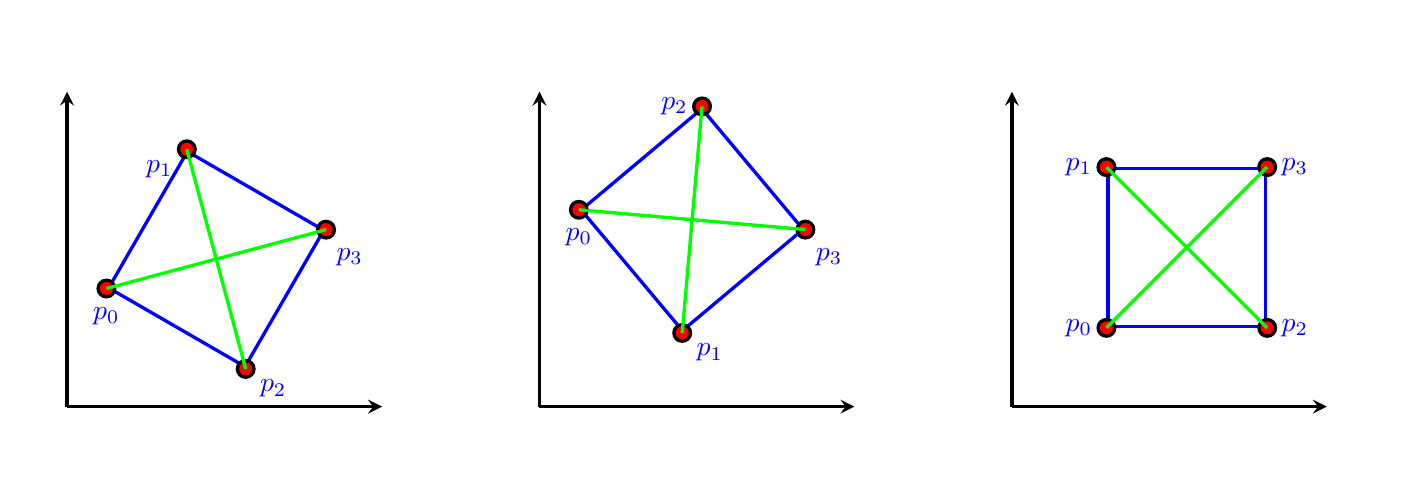
\begin{tikzpicture}
[every node/.style={draw, rectangle, blue, minimum size=2cm}, very thick]
\draw[very thick, >=stealth, ->] (0,0) -- ++(0,4);
\draw[very thick, >=stealth, ->] (0,0) -- ++(4,0);
\node(0) at (0.5, 1.5) [anchor=south west, rotate=-30] {};
\draw[fill=red] (0.south west) circle (3pt);
\draw[fill=red] (0.north west) circle (3pt);
\draw[fill=red] (0.north east) circle (3pt);
\draw[fill=red] (0.south east) circle (3pt);
\node[draw=none] at ($(0.south west) + (0, -3.5mm)$) {$p_0$};
\node[draw=none] at ($(0.north west) + (-3.5mm, -2.5mm)$) {$p_1$};
\node[draw=none] at ($(0.south east) + (3.5mm, -2.5mm)$) {$p_2$};
\node[draw=none] at ($(0.north east) + (3mm, -3.5mm)$) {$p_3$};
\draw[green] (0.south west) -- (0.north east);
\draw[green] (0.south east) -- (0.north west);
\draw[very thick, >=stealth, ->] (6,0) -- ++(0,4);
\draw[very thick, >=stealth, ->] (6,0) -- ++(4,0);
\node(1) at (6.5, 2.5) [anchor=south west, rotate=-50] {};
\draw[fill=red] (1.south west) circle (3pt);
\draw[fill=red] (1.north west) circle (3pt);
\draw[fill=red] (1.north east) circle (3pt);
\draw[fill=red] (1.south east) circle (3pt);
\node[draw=none] at ($(1.south west) + (0, -3.5mm)$) {$p_0$};
\node[draw=none] at ($(1.north west) + (-3.5mm, 0)$) {$p_2$};
\node[draw=none] at ($(1.south east) + (3.5mm, -2.5mm)$) {$p_1$};
\node[draw=none] at ($(1.north east) + (3mm, -3.5mm)$) {$p_3$};
\draw[green] (1.south west) -- (1.north east);
\draw[green] (1.south east) -- (1.north west);
\draw[very thick, >=stealth, ->] (12,0) -- ++(0,4);
\draw[very thick, >=stealth, ->] (12,0) -- ++(4,0);
\node(2) at (13.2, 1) [anchor=south west] {};
\draw[fill=red] (2.south west) circle (3pt);
\draw[fill=red] (2.north west) circle (3pt);
\draw[fill=red] (2.north east) circle (3pt);
\draw[fill=red] (2.south east) circle (3pt);
\node[draw=none] at ($(2.south west) + (-3.5mm, 0)$) {$p_0$};
\node[draw=none] at ($(2.north west) + (-3.5mm, 0)$) {$p_1$};
\node[draw=none] at ($(2.south east) + (3.5mm, 0)$) {$p_2$};
\node[draw=none] at ($(2.north east) + (3.5mm, 0)$) {$p_3$};
\draw[green] (2.south west) -- (2.north east);
\draw[green] (2.south east) -- (2.north west);
\end{tikzpicture}
\end{figure}

In each case, after sorting, we obtain the following conclusion regarding the connections of the points:

\begin{itemize}
\item $(p_0,p_1)$, $(p_1,p_3)$, $ (p_3, p_2)  $,  and $(p_2, p_0)$  form the four sides of any valid square.
\item $(p_0, p_3)$ and $ (p_1, p_2) $ form the diagonals of the square.

\end{itemize}
Thus, once the sorting of the points is done, based on the above knowledge, we can directly compare  $(p_0,p_1)$, $(p_1,p_3)$, $ (p_3, p_2p)  $,  and $(p_2, p_0)$
for equality of lengths(corresponding to the sides); and $(p_0, p_3)$ and $ (p_1, p_2) $ for equality of lengths(corresponding to the diagonals).

\setcounter{lstlisting}{0}
\begin{lstlisting}[style=customc, caption={Sort}]
bool validSquare( vector<int>& p1, vector<int>& p2, vector<int>& p3, vector<int>& p4 )
{
    vector<vector<int>> pts( 4 );

    swap( pts[0], p1 );
    swap( pts[1], p2 );
    swap( pts[2], p3 );
    swap( pts[3], p4 );

    //sort the points per the x-coordinate first
    //if tie, per y-coordinate
    sort( begin( pts ), end( pts ), []( const vector<int>& a, const vector<int>&b )
    {
        if( a[0] < b[0] )
        {
            return true;
        }

        if( a[0] == b[0] )
        {
            return a[1] < b[1];
        }

        return false;
    } );

    //get the square distance
    auto sqd = [&pts]( int a, int b )
    {
        int x = pts[a][0] - pts[b][0];
        int y = pts[a][1] - pts[b][1];
        return x * x + y * y;
    };

    array<int, 4> da;

    da[0] = sqd( 0, 1 );
    da[1] = sqd( 1, 3 );
    da[2] = sqd( 3, 2 );
    da[3] = sqd( 2, 0 );

    //if all values are equal
    //the result will be 4
    int cnt = count( begin( da ), end( da ), da[0] );

    if( ( cnt != 4 ) || ( da[0] == 0 ) )
    {
        //if they are not equal
        //or all have same coordinates
        return false;
    }

    //make sure the diagonal lengths are equal
    return sqd( 0, 3 ) == sqd( 1, 2 );
}
\end{lstlisting}
\section{594 --- Longest Harmonious Subsequence}
We define a harmounious array as an array where the difference between its maximum value and its minimum value is exactly 1.

Now, given an integer array, $A$, you need to find the length of its longest harmonious subsequence among all its possible subsequences.

\paragraph{Example 1:}
\begin{flushleft}

\textbf{Input}: $[1,3,2,2,5,2,3,7]$

\textbf{Output}: 5

\textbf{Explanation}: The longest harmonious subsequence is $[3,2,2,2,3]$.
 

\end{flushleft}

\paragraph{Note:} 

\begin{itemize}
\item The length of the input array will not exceed 20,000.
\end{itemize}

\subsection{Hash Map}
\begin{itemize}
\item We make use of a hash map $M$ which stores the number of times an element occurs in the array. Traverse $A$ and fill $M$ once.
\item After this, we traverse over the keys of $M$. For every key considered, say $k$, we find out if the map contains the $k + 1$. We need not care about $k-1$, because if $k$ is present in the harmonic subsequence, at one time either $k+1$ or $k - 1$ only could be included in the harmonic subsequence. The case of $k$being in the harmonic subsequence will automatically be considered, when $k- 1$ is encountered as the current key.
\item Whenver we find that $k+ 1$ exists in $M$, we determine the count of the current harmonic subsequence as count of $k$ plus count of $k+1$
\end{itemize}

注意,这种方法可以不用考虑$k-1$是因为首先遍历完了$A$。如果要边做遍历,边进行$M$的更新,那么需要同时考虑$k+1$和$k-1$。
\setcounter{lstlisting}{0}
\begin{lstlisting}[style=customc, caption={Hash Map With One Pass}]
int findLHS( vector<int>& nums )
{
    unordered_map<int, int>m;
	
    int res = 0;
	
    for( auto i : nums )
    {
        m[i]++;
        if( m.count( i + 1 ) )
        {
            res = max( res, m[i] + m[i + 1] );
        }
        if( m.count( i - 1 ) )
        {
            res = max( res, m[i] + m[i - 1] );
        }
    }
	
    return res;
}
\end{lstlisting}

\begin{lstlisting}[style=customc, caption={Hash Map With TWo Pass}]
int findLHS( vector<int>& nums )
{
    unordered_map<int, int> m;

    for( int n : nums )
    {
        m[n] += 1;
    }

    int ans = 0;

    for( const auto& p : m )
    {
        //only consider k+1
        if( m.count( p.first + 1 ) )
        {
            ans = ( max )( p.second + m[p.first + 1], ans );
        }
    }

    return ans;
}
\end{lstlisting}
%\include{595}
%\include{596}
%\include{597}
\section{598 --- Range Addition II}
Given an $m \times n$ matrix $M$ initialized with all 0's and several update operations.

Operations are represented by a 2D array, and each operation is represented by an array with two \textbf{positive} integers $a$ and $b$, which means $M[i][j]$ should be \textbf{added by one} for all $0 \leq i < a$ and $0 \leq j < b$.

You need to count and return the number of maximum integers in the matrix after performing all the operations.

\paragraph{Example 1:}

\begin{flushleft}


\textbf{Input}: 

$m = 3$, $n = 3$

\textbf{operations}: $[[2,2],[3,3]]$

\textbf{Output}: 4

\textbf{Explanation}:
 
\textbf{Initially},

$ M = \begin{bmatrix}
0 & 0  & 0 \\
0 & 0 & 0 \\
0 & 0 & 0
\end{bmatrix}$

After performing $[2,2]$, 

$ M = \begin{bmatrix}
1 & 1  & 0 \\
1 & 1 & 0 \\
0 & 0 & 0
\end{bmatrix}$

After performing $[3,3]$,

$ M = \begin{bmatrix}
2 & 2  & 1 \\
2 & 2 & 1 \\
1 & 1 & 1
\end{bmatrix}$

So the maximum integer in $M$ is 2, and there are four of it in $M$. So return 4.

\end{flushleft}

\paragraph{Note:}
\begin{itemize}
\item The range of $m$ and $n$ is $[1,40000]$.
\item The range of $a$ is $[1,m]$, and the range of $b$ is $[1,n]$.
\item The range of operations size won't exceed 10,000.
\end{itemize}

\subsection{Find Minimum}
\begin{itemize}
\item This problem is actually  to find the minimum row and column for all input operations
\end{itemize}

\setcounter{lstlisting}{0}
\begin{lstlisting}[style=customc, caption={Find Minimum}]
int maxCount( int m, int n, vector<vector<int>>& ops )
{
    if( ops.empty() )
    {
        return m * n;
    }

    //get minimum of row and column
    //for all input ops
    vector<int> x = accumulate( next( ops.begin() ), ops.end(),
                                ops[0],
                                []( const vector<int>& a, const vector<int>& b )
    {
        return vector<int> {( min )( a[0], b[0] ), ( min )( a[1], b[1] )} ;
    } );


    return x[0] * x[1];
}
\end{lstlisting}
\section{599 --- Minimum Index Sum of Two Lists}
Suppose Andy and Doris want to choose a restaurant for dinner, and they both have a list of favorite restaurants represented by strings.

You need to help them find out their common interest with the least list index sum. If there is a choice tie between answers, output all of them with no order requirement. You could assume there always exists an answer.

\paragraph{Example 1:}
\begin{flushleft}
\textbf{Input}:

[ Shogun, Tapioca Express, Burger King, KFC ]

[ Piatti, The Grill at Torrey Pines, Hungry Hunter Steakhouse, Shogun ]

\textbf{Output}: [ Shogun ]

\textbf{Explanation}: The only restaurant they both like is Shogun.
\end{flushleft}

\paragraph{Example 2:}

\begin{flushleft}
\textbf{Input}:

[Shogun, Tapioca Express, Burger King, KFC]

[KFC, Shogun, Burger King]

\textbf{Output}: [Shogun]

\textbf{Explanation}: 

The restaurant they both like and have the least index sum is Shogun with index sum 1 ($0+1$).
\end{flushleft}

\paragraph{Note:}
\begin{itemize}
\item The length of both lists will be in the range of $[1, 1000]$.
\item The length of strings in both lists will be in the range of $[1, 30]$.
\item The index is starting from 0 to the list length minus 1.
\item No duplicates in both lists.
\end{itemize}
\end{document}